\documentclass[journal]{IEEEtran}

\usepackage{amsmath,amssymb,amsfonts}
\usepackage{graphicx}
\usepackage{booktabs}
\usepackage{multirow}
\usepackage{algorithm}
\usepackage{algpseudocode}
\usepackage{placeins}
\usepackage{hyperref}
\usepackage{xcolor}
\usepackage{subcaption}
\usepackage{natbib}
\usepackage{soul}
\usepackage{tikz}
\usepackage{stfloats}
\usetikzlibrary{positioning,arrows.meta,fit,backgrounds,calc}

% Yellow-highlighted, PDF-visible TODO marker. Every unresolved item in this
% manuscript is wrapped in \todohl so it can be found by searching the compiled
% PDF for highlighted text, not only by grepping for a LaTeX comment.
\newcommand{\todohl}[1]{\hl{#1}}

% TODO: intended submission venue is still to be decided by the authors.
% (This file was originally formatted for Resources Policy under
% elsarticle; it has since been reformatted to IEEEtran two-column
% style. Re-confirm target-venue citation/formatting requirements
% before submission.)

\renewcommand{\topfraction}{0.85}
\renewcommand{\bottomfraction}{0.85}
\renewcommand{\textfraction}{0.10}
\renewcommand{\floatpagefraction}{0.85}
\renewcommand{\dbltopfraction}{0.9}
\renewcommand{\dblfloatpagefraction}{0.85}
\setcounter{topnumber}{4}
\setcounter{bottomnumber}{4}
\setcounter{totalnumber}{6}

\begin{document}

\title{Does Per-Frequency-Band Graph Learning Help Copper Price Forecasting? A Rigorous Evaluation and a Diagnosis of Isotropic Embedding Collapse}

\author{\IEEEauthorblockN{Anmol Jain and Sibarama Panigrahi}
\IEEEauthorblockA{Department of Computer Science and Engineering\\
National Institute of Technology Rourkela, Odisha, India\\
anmol752005@gmail.com
}}

\IEEEtitleabstractindextext{%
\begin{abstract}
We build a leakage-safe, capacity-matched protocol testing whether VMD-MFGNN, a per-frequency-band graph neural network, improves copper futures forecasting. Across seven models and four horizons on one 2010--2025 chronological split, none beats a zero-forecast baseline on mean absolute error, and the zero-forecast baseline also wins root-mean-squared error at two horizons. We then diagnose why VMD-MFGNN's per-band graphs show no advantage over a pooled alternative. Trained checkpoints reveal the graph embeddings collapsed isotropically, RMS magnitude falling 32-fold, while two independently trained models share embedding directions at cosine similarity above 0.99. Training rescaled the embeddings without ever rotating them toward task-relevant structure. We attribute this to weight decay overwhelming a weak task gradient, since a near-uniform adjacency already suffices. A targeted fix, normalizing embeddings and excluding them from weight decay, mechanically resolves the collapse. The deeper problem persists: corrected embeddings move only 0.6--2.0\% from random initialization, so the adjacency stays statistically indistinguishable from an untrained graph. Separately, several models, including a tuned re-run that first appeared to reverse our negative finding, emitted near-constant, single-sign forecasts whose directional accuracy exactly matched the test period's class frequency for whichever sign they always predicted --- not necessarily the majority class; our flagship illustrative case always predicted the minority (down-day) sign. We retract that apparent reversal once we identified the artifact. We report this as a general finding: directional accuracy is uninterpretable without checking prediction sign concentration and a majority-class null alongside it. Our contribution is therefore an evaluation protocol, not a winning architecture. It includes a disclosed naive-baseline comparison absent from the directly comparable prior work we surveyed, a quantified graph-collapse failure mode relevant to low-node-count financial GNNs, and a warning about what directional accuracy alone can conceal.
\end{abstract}

\begin{IEEEkeywords}
copper price forecasting, graph neural networks, variational mode decomposition, multi-frequency analysis, commodity markets.
\end{IEEEkeywords}}

\maketitle
\IEEEdisplaynontitleabstractindextext
\IEEEpeerreviewmaketitle

\noindent\todohl{[TODO: target submission venue is not yet decided. This
manuscript is currently formatted in IEEEtran two-column journal style; it was
originally drafted for Resources Policy under elsarticle. Re-confirm the target
venue's citation, formatting and length requirements before submission.]}

%% ============================================================
\section{Introduction}
\label{sec:intro}

Copper is among the most economically significant industrial metals, colloquially termed ``Dr.\ Copper'' in financial commentary for its perceived ability to signal macroeconomic health. Global copper output reached approximately 22.8 million metric tonnes in 2024, with China consuming over 50\% of global demand \citep{IEA2024}. The ongoing energy transition---electric vehicles require 53--83\,kg of copper per unit versus 15--23\,kg for internal combustion engines---is creating structural demand shifts that complicate traditional forecasting approaches \citep{IEA2024}. Forecasting errors translate directly into hedging and inventory decisions across the copper supply chain: mine operators and smelters price forward sales off short-horizon forecasts, while EV and grid-infrastructure manufacturers plan multi-year procurement off longer-horizon ones, so both the accuracy and the honesty of a forecasting method's reported accuracy matter in a way that is specific to this market, not generic to commodities.

Recent advances in copper price forecasting have progressed along two largely overlapping tracks. The first track employs signal decomposition methods, particularly Variational Mode Decomposition (VMD), to separate copper price series into frequency components before forecasting each independently. VMD-LSTM \citep{Liu2020} established the benchmark and is, as of this writing, the most-cited paper in this specific sub-area (290 citations per Google Scholar, accessed 2026-08), and secondary decomposition approaches (e.g., CEEMDAN+VMD) represent the current frontier \citep{Zhang2025a, ZhangKe2025}. Most of these methods treat copper as an isolated univariate series, discarding the inter-commodity dependencies that drive prices, although a small number of very recent papers now combine VMD with graph neural networks (Section~\ref{sec:related}).

The second track applies Graph Neural Networks (GNN) to model cross-asset relationships. GNNs have shown strong results in stock prediction \citep{Cheng2022, Qian2024} and have recently been applied to copper via a Multi-view Graph Transformer \citep{Sun2025}, which constructs a single graph over undecomposed prices. Separately, at least one recent paper, MBTI-Net \citep{LiLiu2026}, combines VMD decomposition with a GNN for copper futures, but pools the decomposed modes into a single graph rather than constructing one graph per frequency band. In both cases, a single graph structure collapses whatever multi-scale dependency structure exists across frequency bands into one static representation.

The premise motivating a per-band graph is intuitive and, on its face, plausible: commodity relationships are plausibly multi-scale, so the copper-dollar correlation at low frequencies (reflecting long-term macroeconomic co-movement) may differ structurally from the copper-dollar relationship at high frequencies (reflecting daily trading noise), and a single graph, pooled or otherwise, cannot represent both simultaneously. \textbf{This paper does not assume that premise; it tests it.} We built VMD-MFGNN, a Multi-Frequency Graph Neural Network that constructs a \emph{separate} learned inter-variable graph for each VMD frequency band, exactly the architectural distinction MBTI-Net-style pooling forgoes, and evaluate it against six baselines and a matched pooled-graph ablation under a leakage-safe, capacity-disclosed protocol. We report what we found even where it complicates the paper's own premise: none of the seven models tested, including VMD-MFGNN, beats a trivial zero-forecast baseline on mean absolute error at any horizon, and direct inspection of the trained model's learned graphs shows the per-band mechanism did not learn differentiated relational structure at all---its embeddings collapsed toward a degenerate, near-uniform solution during training, a failure mode we diagnose quantitatively in Section~\ref{sec:collapse}. This reframes the paper's contribution from an architectural proposal to an evaluation study with a diagnosed negative result.

VMD-MFGNN (\textbf{V}ariational \textbf{M}ode \textbf{D}ecomposition \textbf{M}ulti-\textbf{F}requency \textbf{G}raph \textbf{N}eural \textbf{N}etwork):

\begin{enumerate}
    \item Decomposes an 8-variable commodity/macro time series into $K=5$ frequency bands via VMD, using a leakage-safe rolling window refit at every trading day;
    \item Constructs a \emph{separate} learned inter-variable graph at each frequency band, intended to capture scale-dependent cross-commodity dependencies;
    \item Applies Graph Attention Networks (GAT) per frequency band for spatial modeling and an LSTM for temporal modeling;
    \item Fuses band-level predictions via learned attention weights.
\end{enumerate}

This paper is organized around four research questions, posed here before any results are reported so that Section~\ref{sec:discussion}'s answers have a clear antecedent:
\begin{itemize}
    \item \textbf{RQ0}: Does any model tested here, including VMD-MFGNN, beat a trivial zero-forecast (do-nothing) baseline?
    \item \textbf{RQ1}: Does constructing a separate learned graph per frequency band outperform pooling the bands into a single graph?
    \item \textbf{RQ2}: Does VMD decomposition, and does end-to-end learned (versus fixed correlation-based) adjacency, add measurable value over the alternatives?
    \item \textbf{RQ3}: Does VMD-MFGNN differ significantly, in the Diebold-Mariano sense, from standard forecasting baselines?
\end{itemize}

Our contributions are:
\begin{itemize}
    \item \textbf{A rigorous, leakage-safe, capacity-matched evaluation protocol}, applied to a question this literature rarely asks explicitly: does VMD decomposition and per-band graph learning add measurable forecasting value over standard baselines and a trivial naive benchmark, for copper returns at this data scale? The protocol includes a capacity-disclosed six-variant ablation (Section~\ref{sec:ablation}), a Diebold-Mariano significance test with a multiple-testing correction (Section~\ref{sec:experiments}), and, critically, a naive random-walk baseline comparison, which we did not find reported in any of the eleven most directly comparable works surveyed in Table~\ref{tab:related} (Section~\ref{sec:results}). Our reason for building the protocol first and treating the architecture as the object under test is the pattern \citet{KapoorNarayanan2022} document across seventeen scientific fields and hundreds of papers: leakage and evaluation shortcuts, rather than modelling choices, are the dominant driver of irreproducible ML-based scientific claims, and they are typically invisible to a reader of the finished paper. This study's own history bears that out from both directions --- a leaky VMD decomposer was caught and replaced before any reported result was produced (Section~\ref{sec:method}), and a later re-run that appeared to reverse this paper's central negative finding turned out to be an evaluation artifact rather than a real effect (Section~\ref{sec:constantforecast}).
    \item \textbf{A diagnosed, quantified mechanistic account of why the proposed graph-learning mechanism failed to produce useful structure}, not just an observation that it did: we trace the per-band adjacency's collapse to uniform edge weights to isotropic norm decay in the underlying graph embeddings during training, rule out the more obvious dead-ReLU explanation with a direct test, and identify the likely optimization dynamic responsible (Section~\ref{sec:collapse}). This is offered as a citable finding relevant to other low-node-count learned-graph architectures in financial GNN research, including MBTI-Net-style designs, not only to this paper's own model.
    \item \textbf{An honest reference point most comparison papers in this area omit}: every model in this study, including the proposed one, is compared directly against a trivial zero-forecast baseline, and we report plainly that none beats it on mean absolute error at any horizon (Section~\ref{sec:results}).
    \item \textbf{A targeted, verified fix for the diagnosed collapse, and an honest account of its limits}: we engineer and test a specific intervention (unit-normalizing the graph embeddings before the bilinear product and excluding them from weight decay), confirm it mechanically resolves the norm-collapse mechanism, and show the underlying embeddings still fail to learn any task-relevant structure once the collapse itself is removed as an explanation---strengthening, not merely repeating, the earlier diagnosis (Section~\ref{sec:graphfix}).
    \item \textbf{A general methodological finding about directional accuracy}: several models across this study's experiments, including a re-run originally thought to reverse the paper's central negative result, turn out to be emitting near-constant forecasts whose apparent directional accuracy is an artifact of the test period's majority class rather than a measurement of directional skill---a failure mode invisible to a bare directional-accuracy percentage and only caught by checking prediction sign concentration and a majority-class null directly (Section~\ref{sec:constantforecast}). We developed this check independently, but claim no priority for the underlying base-rate concern, which \citet{Cheung2026} raises for equity forecasting; what we add is the sign-concentration and base-rate-identity machinery that detects a \emph{degenerate forecaster}, not only a misspecified null, and can be applied retroactively to already-reported results (Section~\ref{sec:constantforecast}).
\end{itemize}

%% ============================================================
\section{Related Work}
\label{sec:related}

\subsection{Copper Price Forecasting}

Traditional approaches include ARIMA \citep{Becerra2022}, GARCH \citep{Garcia2019}, and VAR/VECM models \citep{Dai2025}. Machine learning methods---LSTM \citep{Hu2020, Luo2022}, CNN-LSTM \citep{Li2023}, XGBoost \citep{Nabavi2024}, and Transformers \citep{Tseng2025, Zhao2025}---have shown improvements over econometric baselines, particularly at longer horizons.

\subsection{Decomposition-Ensemble Methods}

Signal decomposition followed by component-wise forecasting is the most active methodological area. VMD-LSTM \citep{Liu2020} is, to our knowledge, the most-cited work specifically combining VMD with LSTM forecasting for non-ferrous metals, demonstrating that VMD's variational formulation avoids the mode mixing issues of EMD/EEMD \citep{Dragomiretskiy2014}. Recent advances include secondary decomposition \citep{LiuLiu2022, Zhang2025a}, adaptive VMD parameter selection \citep{ZhangKe2025}, and complexity-aware decomposition \citep{LiLiu2026}. The large majority of decomposition-ensemble methods treat variables independently, discarding cross-variable information.

\subsection{Graph Neural Networks for Financial Forecasting}

MTGNN \citep{Wu2020mtgnn} introduced learned adaptive adjacency matrices for multivariate time series, and our per-band graph construction (Section~\ref{sec:graph}) follows the same adjacency parameterization applied independently within each frequency band. StemGNN \citep{Cao2020} operates in the joint spectral-temporal domain. FourierGNN \citep{Yi2023} unifies spatial and temporal modeling via Fourier operators. In finance, THGNN \citep{Xiang2023} uses dynamic heterogeneous graphs for stocks, and MDGNN \citep{Qian2024} introduces multi-relational dynamic graphs.

For commodities specifically, the literature is sparse. \citet{Sun2025} proposed a Multi-view Graph Transformer for copper that constructs a single graph over undecomposed price data---the graph structure does not vary by frequency scale. \citet{Hu2023} applied heterogeneous continual GNN to 49 Chinese futures contracts. \citet{Zhai2024} used a Graph Fourier Transformer for base metals.

\subsection{VMD Combined with GNN, and Positioning of This Work}

A small number of papers combine VMD with GNN, mostly outside finance: traffic forecasting \citep{Ahmad2024, Ahmad2025}, air quality \citep{Pei2022}, wind energy \citep{ChengTsai2026, Bao2025}, and industrial applications \citep{Yuan2025}. Within finance, \citet{LiLiu2026} (``MBTI-Net'') combines VMD decomposition with a GNN for copper futures price forecasting; this is the closest prior work to ours and rules out any claim of being first to combine VMD and GNNs for copper. Critically, MBTI-Net pools the decomposed VMD modes into a single unified graph before applying graph convolution---the graph topology does not vary across frequency bands. \citet{ZhengZhufu2025} combine DCT (not VMD) with a cross-scale GNN for single-stock prediction, not multi-commodity relational modeling.

The gap we target is therefore precise: among work that combines signal decomposition with graph-based relational modeling for commodity or financial time series, we are not aware of any that constructs a \emph{separate} graph per decomposed frequency band across a multi-commodity system, as opposed to (a) pooling bands into one graph (MBTI-Net) or (b) using a single graph over undecomposed data (Sun et al., 2025). Table~\ref{tab:related} makes this positioning checkable against the most directly comparable prior work discussed above, rather than only argued in prose. We do not claim priority over VMD+GNN combinations generally, nor over GNN applications to copper generally.

\begin{table}[t]
\centering
\caption{Positioning against the most directly comparable prior work. ``Per-band graph'' means a separate learned adjacency per frequency/scale component; ``pooled/single'' means one graph shared across components or over undecomposed data.}
\label{tab:related}
\small
\begin{tabular}{@{}p{1.75cm}cp{2.3cm}p{1.65cm}@{}}
\toprule
Work & Decomp.? & Graph & Domain \\
\midrule
VMD-LSTM \citep{Liu2020} & VMD & --- & metals (univar.) \\
MTGNN \citep{Wu2020mtgnn} & --- & learned, single & multiv.\ TS \\
StemGNN \citep{Cao2020} & spectral & learned, single & multiv.\ TS \\
FourierGNN \citep{Yi2023} & Fourier & learned, single & multiv.\ TS \\
THGNN \citep{Xiang2023} & --- & dynamic, single & stocks \\
MDGNN \citep{Qian2024} & --- & multi-relational & stocks \\
Sun et al.\ \citeyear{Sun2025} & --- & single, undecomp. & copper \\
Hu et al.\ \citeyear{Hu2023} & --- & heterog., single & futures (49) \\
Zhai et al.\ \citeyear{Zhai2024} & Fourier & learned, single & base metals \\
Zheng \& Zhufu \citeyear{ZhengZhufu2025} & DCT & cross-scale, single & single stock \\
MBTI-Net \citep{LiLiu2026} & VMD & \textbf{pooled} & copper \\
\textbf{This work} & VMD & \textbf{per-band ($K{=}5$)} & copper (multi.) \\
\bottomrule
\end{tabular}
\end{table} More importantly, we do not simply assert that the per-band choice is an improvement over MBTI-Net-style pooling and leave it there: we treat it as an empirical question MBTI-Net's architecture implicitly answers one way (pooling is sufficient) without testing the alternative, and we test both sides of that question directly, against a matched pooled-graph baseline (Section~\ref{sec:ablation}), at the same data scale. Our result complicates a straightforward reading of MBTI-Net's design choice: we find no ablation evidence that per-band graphs outperform pooling, and we go further than reporting that negative comparison by diagnosing \emph{why} it comes out this way---the per-band graph-learning mechanism in our model collapsed to near-uniform edge weights during training (Section~\ref{sec:collapse}), a specific, quantified failure mode that, to our knowledge, has not previously been documented for this class of learned-adjacency GNN architecture at low node counts. It is not, however, without precedent, and we do not present it as unanticipated: \citet{Fountoulakis2023} prove, and confirm on both synthetic and real graphs, that in a low signal-to-noise (``hard'') regime of the contextual stochastic block model, a graph attention network's coefficients concentrate on uniform $1/|\mathcal{N}_i|$ weights, so the attention mechanism reduces to ordinary mean-aggregating graph convolution and cannot distinguish important from unimportant edges. Their setting is attention over a \emph{given} graph in node classification, and their mechanism is the statistical indistinguishability of intra- from inter-class edges rather than an optimization dynamic; ours is a \emph{learned} bilinear adjacency in a forecasting model, degenerating for a different, traceable reason (Section~\ref{sec:collapse}). The qualitative endpoint --- graph attention collapsing to uniform weights when there is too little signal to differentiate edges --- is nonetheless the same, which we take as corroborating rather than diminishing the finding. This does not establish that MBTI-Net's own pooled graph suffers the same failure---we did not have access to retrain or inspect MBTI-Net's checkpoints---but it is a concrete, mechanistic reason to be skeptical that per-band-versus-pooled is a distinction that reliably matters at this problem scale, and a more informative contribution to that specific architectural question than either an unexamined win or an unexamined loss would be.

%% ============================================================
\section{Methodology}
\label{sec:method}

\subsection{Problem Formulation}

Given $N=8$ multivariate time series $\{\mathbf{x}_1, \ldots, \mathbf{x}_N\}$ representing copper price and related commodity/macroeconomic variables, we aim to forecast the copper price return $r_{t+h} = \ln(p_{t+h}/p_t)$ at horizons $h \in \{1, 5, 10, 22\}$ trading days, using a lookback window of $L$ timesteps. We state the exact indexing convention once here since it is easy to get subtly wrong: the window used to predict $r_{t+h}$ spans timesteps $t-L,\ldots,t-1$ (strictly before $t$, the day the forecast is issued from), not $t-L+1,\ldots,t$; this is the same convention the ARIMA baseline documents explicitly in its implementation, and every model in this study uses it identically, so it does not affect any cross-model comparison, but every forecast horizon is effectively one trading day longer in wall-clock terms than the horizon label alone would suggest. Table~\ref{tab:notation} collects the symbols used across this section and Sections~\ref{sec:collapse} and~\ref{sec:robustness}, since the notation is dense enough that we found it worth fixing in one place rather than only at each symbol's first use.

\begin{table}[t]
\centering
\caption{Notation used in Sections~\ref{sec:method}, \ref{sec:collapse}, and \ref{sec:robustness}.}
\label{tab:notation}
\small
\begin{tabular}{@{}lp{6.3cm}@{}}
\toprule
Symbol & Meaning (fixed value in this paper) \\
\midrule
$N$ & number of input variables ($N=8$) \\
$K$ & number of VMD frequency bands ($K=5$; swept $\{3,5,7,9\}$ in Section~\ref{sec:robustness}) \\
$L$ & lookback window length ($L=60$ trading days) \\
$T$ & total series length (lookback timestep index range) \\
$d$ & graph-embedding dimension ($d=16$, fixed, not HPO-searched) \\
$d_h$ & hidden dimension (64 default; 32/64/128 HPO-searched) \\
$H$ & number of GAT attention heads (4 default; 2/4/8 HPO-searched) \\
top-$k$ & per-row adjacency sparsification budget ($k=4$ of $N=8$) \\
$\mathcal{H}$ & forecast horizon set, $\{1,5,10,22\}$ trading days \\
$\mathbf{A}_k$ & learned adjacency matrix for band $k$ \\
$\mathbf{E}^{(1)}_k,\mathbf{E}^{(2)}_k$ & bilinear graph-embedding matrices for band $k$, $\in\mathbb{R}^{N\times d}$ \\
$\mathbf{z}^{(k)}$ & band-$k$ representation after GAT+LSTM \\
$w_k$ & attention-fusion weight for band $k$ \\
\bottomrule
\end{tabular}
\end{table}

\subsection{Variational Mode Decomposition}

VMD \citep{Dragomiretskiy2014} decomposes a signal $f(t)$ into $K$ band-limited intrinsic mode functions $\{u_k\}_{k=1}^{K}$ by solving:
\begin{equation}
\min_{\{u_k\}, \{\omega_k\}} \sum_{k=1}^{K} \left\| \partial_t \left[ \left(\delta(t) + \frac{j}{\pi t}\right) * u_k(t) \right] e^{-j\omega_k t} \right\|_2^2 \quad \text{s.t.} \quad \sum_{k=1}^{K} u_k = f
\end{equation}
where $\omega_k$ is the center frequency of mode $k$. The constrained problem is solved via ADMM in the Fourier domain with penalty parameter $\alpha$.

We apply VMD independently to each of the $N=8$ input variables with $K=5$ modes, yielding a tensor of modes $\mathbf{U} \in \mathbb{R}^{N \times K \times T}$. To prevent temporal leakage, decomposition uses a \emph{rolling window, refit at every trading day}: at trading day $t$, VMD is recomputed from scratch on the window of the most recent 252 trading days ending at and including $t$ (\texttt{signal[max(0,t-251):t+1]}), never using data beyond $t$, and only the final-timestep value of each resulting mode is retained as day $t$'s feature. Because refitting happens at every single day rather than periodically, each mode's assigned series is a genuinely daily-varying signal at the same temporal resolution as the raw price data, not a value held constant across a multi-day block. Because VMD's ADMM optimization does not guarantee a consistent mode ordering across independent daily fits, each day's $K$ modes are re-sorted by ascending converged center frequency ($\omega_k$) before being stored, so mode index 0 is always the lowest-frequency band and mode $K-1$ the highest, consistently across the full time series. An earlier version of this pipeline instead used an expanding-window decomposer that refit only every 21 trading days and carried the resulting modes forward (constant) across each 21-day block; that design was found to collapse a 60-day lookback window into as few as three distinct feature values per variable/mode and was replaced by the daily-refit rolling-window design described above before any of the results in this paper were produced. The concern this design addresses is not idiosyncratic to this study: \citet{Feng2026} independently identify temporal leakage in VMD-based forecasting as a general problem in the electricity-demand literature --- noting that decomposing an entire series, or even an entire input subsequence, before forecasting grants the model access to future information --- and adopt a sample-wise, rolling-window VMD scheme for the same causality-preserving reason we adopt a daily-refit one here. Decomposed modes and refit metadata (split dates, VMD parameters, the rolling-window length, and a hash of the underlying price data) are cached to disk, with cache invalidation triggered by any change to the underlying data or parameters.

\subsection{Frequency-Specific Graph Construction}
\label{sec:graph}

The central architectural choice in VMD-MFGNN is constructing a \emph{separate} graph $G_k = (V, E_k)$ for each frequency band $k \in \{1,\ldots,K\}$, where nodes $V = \{1, \ldots, N\}$ represent the $N=8$ variables and edges $E_k$ capture band-specific inter-variable dependencies. This is directly contrasted, via ablation, against a single graph pooled across all $K$ bands (Section~\ref{sec:ablation}).

We employ learned adaptive adjacency matrices following \citet{Wu2020mtgnn}, applied independently within each band. For each band $k$, two embedding matrices $\mathbf{E}^{(1)}_k, \mathbf{E}^{(2)}_k \in \mathbb{R}^{N \times d}$ are randomly initialized and jointly optimized:
\begin{equation}
\label{eq:graph}
\mathbf{A}_k = \text{softmax}\left(\text{ReLU}\left(\mathbf{E}^{(1)}_k {\mathbf{E}^{(2)}_k}^\top\right)\right)
\end{equation}
(the implementation applies no $1/\sqrt{d}$ scaling to the bilinear logits before ReLU/softmax; we state this explicitly because this absence turns out to matter for the collapse mechanism diagnosed in Section~\ref{sec:collapse}). Each row of $\mathbf{A}_k$ is then sparsified to its top-$k=4$ entries (out of $N=8$), so the realized per-band graph is not fully connected; the complexity analysis in Section~\ref{sec:complexity} accounts for this sparsification. This produces $K$ adjacency matrices, one per frequency band, each intended to capture dependencies at its own frequency scale. As an ablation-only alternative (Section~\ref{sec:ablation}), the learned adjacency can be replaced by a fixed, precomputed adjacency built from Pearson correlation between variables' band signals, thresholded at $|r| > 0.3$ (edges below this magnitude are dropped, following a conventional weak-to-moderate correlation cutoff). We note two implementation details of this fixed graph, since they mean it is not a drop-in magnitude-only replacement for the learned adjacency: the retained entries keep their \emph{signed} correlation value (negative correlations reach the GAT layer as negative edge features, unlike the learned adjacency's post-softmax non-negative weights), and the diagonal is fixed at 1.0 (a self-loop 3--8$\times$ larger than any retained off-diagonal entry), whereas the learned path instead receives GAT's own mean-valued self-loops. Both are held constant across all reported correlation-graph results, so they do not confound the correlation-graph ablation's own reported numbers, but a reader comparing it directly against the learned-adjacency mechanism should be aware the two are not scaled identically. The correlation matrices themselves are computed once, from the training split only, and frozen for the remainder of that run (validation and test batches reuse the same frozen matrices rather than recomputing their own), so this ablation does not leak test- or validation-period correlation structure into the graph it is scored against.

\subsection{Frequency Band Module}

For each band $k$, a \textbf{FrequencyBandModule} processes the $k$-th modes of all $N$ variables:

\textbf{Graph Attention Layer.} At each timestep $t$, the mode values $\mathbf{u}^{(k)}_t \in \mathbb{R}^{N}$ are projected to hidden dimension $d_h$ and processed by a multi-head Graph Attention Network (GAT) \citep{Velickovic2018}:
\begin{equation}
\label{eq:gat}
\mathbf{h}^{(k)}_{t} = \text{GAT}(\mathbf{u}^{(k)}_{t}, \mathbf{A}_k) + \mathbf{u}^{(k)}_{t}
\end{equation}
with residual connections and layer normalization, stacked over \texttt{num\_gnn\_layers} GAT layers. We write $\text{GAT}(\mathbf{u}^{(k)}_t, \mathbf{A}_k)$ for brevity, but $\mathbf{A}_k$ does not act as a fixed aggregation weight the way it would in a GCN: the implementation (PyTorch Geometric's \texttt{GATConv} with \texttt{edge\_dim=1}) uses $\mathbf{A}_k$'s top-$k$-sparsified entries only to fix which edges exist, passing each kept edge's weight in as a scalar edge feature; the GAT layer then computes its own attention coefficient for every edge from the node features and that edge feature jointly, and it is this learned attention coefficient, not $\mathbf{A}_k$ directly, that weights the message passed along the edge. Collapse of $\mathbf{A}_k$ to near-uniform values (Section~\ref{sec:collapse}) therefore removes the edge-feature signal GAT's attention could otherwise use to differentiate edges, rather than literally forcing uniform aggregation weights, though the two are observed to coincide in practice (Section~\ref{sec:collapse}).

\textbf{Temporal Layer.} The GAT-enhanced representations are fed to a multi-layer LSTM across the temporal dimension, applied independently per variable, to capture sequential dependencies:
\begin{equation}
\mathbf{z}^{(k)} = \text{LSTM}(\mathbf{h}^{(k)}_{1}, \ldots, \mathbf{h}^{(k)}_{L})
\end{equation}

The output for the target variable (copper, node 0) is $\mathbf{z}^{(k)}_{\text{Cu}} \in \mathbb{R}^{d_h}$.

Algorithm~\ref{alg:vmdmfgnn} summarizes the full forward pass just described, from raw multivariate input through per-band graph construction and GAT+LSTM processing to the fusion and prediction steps detailed in the remainder of this section, and Figure~\ref{fig:architecture} renders the same forward pass as a block diagram with tensor shapes and the per-band repetition made explicit. The two are intended to be read together: every block in the figure corresponds to one or more numbered lines of the algorithm, and the figure adds no component the algorithm does not specify. It describes the architecture as designed; whether the per-band graph mechanism (lines 4--7) learns the differentiated structure it is intended to is an empirical question taken up separately in Section~\ref{sec:collapse}.

\begin{figure*}[!t]
\centering
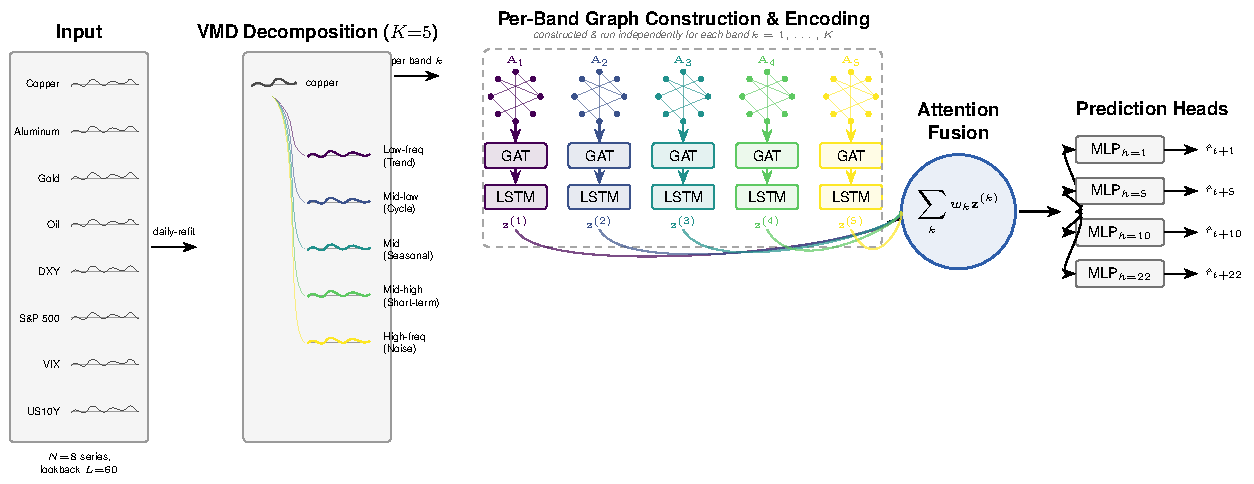
\includegraphics[width=\textwidth]{figures/architecture_diagram.pdf}
\caption{VMD-MFGNN forward pass. An $N=8$ variable window of length $L=60$ trading days (copper, aluminum, gold, oil, DXY, S\&P 500, VIX, US10Y) is decomposed by leakage-safe daily-refit VMD into $K=5$ frequency-band modes, reusing the same band names and colors as Figure~\ref{fig:vmd}. \textbf{The five colored node-link icons are this paper's central architectural claim made visible}: a separate learned graph $\mathbf{A}_k$ is constructed independently for each band (dashed group), each with its own bilinear embedding pair $\mathbf{E}^{(1)}_k,\mathbf{E}^{(2)}_k$ (Eq.~\ref{eq:graph}), row-sparsified to top-$k=4$ of $N=8$ edges, and fed to that band's own GAT and LSTM (Eq.~\ref{eq:gat}). The five resulting representations $\mathbf{z}^{(k)}$ are combined by learned-query attention fusion and mapped to the four forecast horizons by separate heads. Algorithm~\ref{alg:vmdmfgnn} gives the same forward pass line-by-line; the pooled-graph ablation of Section~\ref{sec:ablation} replaces the five per-band graphs shown here with a single graph shared across bands (Figure~\ref{fig:perband-vs-pooled}). Section~\ref{sec:collapse} shows that, once trained, all five $\mathbf{A}_k$ collapse to a near-uniform graph indistinguishable from an untrained one.}
\label{fig:architecture}
\end{figure*}

\begin{algorithm}[!t]
\caption{VMD-MFGNN forward pass}
\label{alg:vmdmfgnn}
\begin{algorithmic}[1]
\Require Raw multivariate window $\{\mathbf{x}_1,\ldots,\mathbf{x}_N\}$ for $N=8$ variables over lookback $L=60$; number of frequency bands $K=5$; adjacency sparsification parameter top-$k=4$; embedding dimension $d$; hidden dimension $d_h$; number of GAT heads $H$; forecast horizons $\mathcal{H}=\{1,5,10,22\}$
\Ensure Predicted returns $\{\hat{r}_{t+h}\}_{h\in\mathcal{H}}$
\State \textbf{VMD decomposition:} for each variable $n=1,\ldots,N$, decompose the rolling window ending at $t-1$ (i.e.\ the $L$ most recent timesteps strictly before the day the forecast is issued from, following this paper's dataset indexing convention) into $K$ band-limited modes via leakage-safe daily-refit VMD, sort modes by ascending center frequency $\omega_k$, and retain the final-timestep value to form $\mathbf{U} \in \mathbb{R}^{N \times K \times L}$
\For{$k = 1$ to $K$}
    \State \textbf{Graph construction:} initialize (or retrieve) embeddings $\mathbf{E}^{(1)}_k, \mathbf{E}^{(2)}_k \in \mathbb{R}^{N \times d}$
    \State Compute adjacency logits $\mathbf{A}_k \leftarrow \text{softmax}(\text{ReLU}(\mathbf{E}^{(1)}_k {\mathbf{E}^{(2)}_k}^\top))$
    \State Sparsify: retain only each row's top-$k=4$ entries of $\mathbf{A}_k$, zeroing the rest
    \State \textbf{Band processing:} project band-$k$ mode values $\mathbf{u}^{(k)}_t \in \mathbb{R}^N$ to hidden dimension $d_h$
    \For{$t = 1$ to $L$}
        \State $\mathbf{h}^{(k)}_{t} \leftarrow \text{GAT}(\mathbf{u}^{(k)}_{t}, \mathbf{A}_k) + \mathbf{u}^{(k)}_{t}$ (residual, layer norm, stacked over \texttt{num\_gnn\_layers} GAT layers)
    \EndFor
    \State $\mathbf{z}^{(k)} \leftarrow \text{LSTM}(\mathbf{h}^{(k)}_{1}, \ldots, \mathbf{h}^{(k)}_{L})$
    \State Extract copper's representation $\mathbf{z}^{(k)}_{\text{Cu}} \in \mathbb{R}^{d_h}$ (node 0 of $\mathbf{z}^{(k)}$)
\EndFor
\State \textbf{Mode fusion:} for $k=1,\ldots,K$, compute $w_k \leftarrow \exp(\mathbf{q}^\top \mathbf{W}\mathbf{z}^{(k)}_{\text{Cu}}) / \sum_{j=1}^{K} \exp(\mathbf{q}^\top \mathbf{W}\mathbf{z}^{(j)}_{\text{Cu}})$
\State $\mathbf{z}_{\text{fused}} \leftarrow \sum_{k=1}^{K} w_k \cdot \mathbf{z}^{(k)}_{\text{Cu}}$
\For{each horizon $h \in \mathcal{H}$}
    \State $\hat{r}_{t+h} \leftarrow \text{MLP}_h(\mathbf{z}_{\text{fused}})$
\EndFor
\State \Return $\{\hat{r}_{t+h}\}_{h\in\mathcal{H}}$
\end{algorithmic}
\end{algorithm}

\subsection{Attention-Based Mode Fusion}

The $K$ band-level representations are fused via a learned attention mechanism:
\begin{equation}
w_k = \frac{\exp(\mathbf{q}^\top \mathbf{W}\mathbf{z}^{(k)}_{\text{Cu}})}{\sum_{j=1}^{K} \exp(\mathbf{q}^\top \mathbf{W}\mathbf{z}^{(j)}_{\text{Cu}})}, \qquad \mathbf{z}_{\text{fused}} = \sum_{k=1}^{K} w_k \cdot \mathbf{z}^{(k)}_{\text{Cu}}
\end{equation}
where $\mathbf{q}$ is a learnable query vector and $\mathbf{W}$ is a single learned linear projection (not a multi-layer network) applied to each band representation before the query dot product. The attention weights $\{w_k\}$ are intended to be interpretable as revealing which frequency bands contribute most to the prediction; Section~\ref{sec:results} reports how peaked or uniform they turn out to be in practice.

\subsection{Prediction and Training}

Separate two-layer MLP heads (one per horizon, \texttt{Linear}$\to$ReLU$\to$Dropout$\to$\texttt{Linear}, not a single linear layer) map $\mathbf{z}_{\text{fused}}$ to predictions:
$\hat{r}_{t+h} = \text{MLP}_h(\mathbf{z}_{\text{fused}})$. The model is trained end-to-end with MSE loss summed across the four horizons:
\begin{equation}
\mathcal{L} = \sum_{h \in \mathcal{H}} \frac{1}{|\mathcal{T}|} \sum_{t \in \mathcal{T}} (r_{t+h} - \hat{r}_{t+h})^2
\end{equation}
The best-validation-loss checkpoint is selected and used for all reported models (Section~\ref{sec:impl}).

\subsection{Complexity Analysis}
\label{sec:complexity}

Let $N=8$ be the number of variables, $T=L$ the lookback window length ($L=60$ trading days throughout this paper, Section~\ref{sec:impl}), $K=5$ the number of VMD modes, $d_h$ the hidden dimension, and $H$ the number of GAT attention heads. Within one frequency band, the learned adjacency $\mathbf{A}_k$ is top-$k$ sparsified to each node's $k=4$ highest-weight outgoing edges (Section~\ref{sec:graph}) before being passed to the GAT layer, so the graph each band's GAT operates on has $O(Nk)$ edges rather than $O(N^2)$; we report the sparsified-graph cost here rather than the looser fully-connected upper bound. This gives per-timestep GAT cost $\mathcal{O}(Nk\,d_h/H)$ for the attention computation and $\mathcal{O}(N d_h^2)$ for the linear projections, repeated over $T$ timesteps and \texttt{num\_gnn\_layers} GAT layers; the per-variable LSTM that follows costs $\mathcal{O}(N T d_h^2)$. Because this cost is incurred independently for each of the $K$ bands, VMD-MFGNN's total forward-pass cost is $\mathcal{O}(K(Nk\,T d_h + N T d_h^2))$, i.e., $K\times$ the cost of a single-graph architecture with otherwise identical per-band capacity. This is the direct computational price of per-band graph construction, and is the reason the pooled-graph ablation (Section~\ref{sec:ablation}) is evaluated as a single-graph, single-pass alternative rather than dismissed a priori as architecturally uninteresting.

Two distinct trained instances of the VMD-MFGNN architecture appear in this paper, and their parameter counts must not be conflated. The main comparison (Section~\ref{sec:results}) uses the HPO-tuned configuration selected by the search in Section~\ref{sec:hpo} ($d_h=128$, $H=2$, \texttt{num\_gnn\_layers}$=1$), which has \textbf{1{,}461{,}124} trainable parameters, counted directly from the saved, trained model. The ablation study (Section~\ref{sec:ablation}) instead uses the untuned default configuration ($d_h=64$, $H=4$, \texttt{num\_gnn\_layers}$=2$, per Section~\ref{sec:impl}) for its \texttt{full\_model} row, which has \textbf{393{,}476} trainable parameters, likewise counted from its own saved, trained checkpoint. HPO is applied only to the main-table model, never to the ablation variants (Section~\ref{sec:hpo}); consequently the ablation table's \texttt{full\_model} is a genuinely different, smaller model instance than the main table's VMD-MFGNN row, not the same trained model reused across tables. This is a deliberate, disclosed design choice, not an inconsistency: re-running HPO separately for every ablation variant was judged infeasible within the project's compute budget, and holding the ablation variants at one fixed, shared default configuration keeps the ablation comparison internally consistent even though it is not directly comparable in absolute terms to the main table.

Within the ablation study, capacity is controlled two ways for the no-VMD and pooled-graph variants, and the resulting real parameter counts (from the trained checkpoints) are reported here rather than estimated: a \emph{matched-dimension} variant that keeps the full model's $d_h$ fixed and lets parameter count fall out of the architecture (\texttt{pooled\_graph\_matched\_dim}: 84{,}618 params, $-$78.5\% vs.\ \texttt{full\_model}; \texttt{no\_vmd\_raw\_price\_matched\_dim}: 88{,}836 params, $-$77.4\%), and a \emph{matched-parameter} variant that increases $d_h$ until total parameter count is approximately restored to \texttt{full\_model}'s (\texttt{pooled\_graph\_matched\_params}: 397{,}586 params, $+$1.05\%; \texttt{no\_vmd\_raw\_price\_matched\_params}: 394{,}116 params, $+$0.16\%). The matched-parameter variants land within about 1\% of \texttt{full\_model}'s parameter count, confirming the capacity-matching procedure worked as intended at real data scale. \texttt{correlation\_graph} (392{,}196 params, $-$0.33\%), which keeps the full per-band architecture and only replaces the learned adjacency with a fixed correlation-threshold graph, is essentially parameter-matched to \texttt{full\_model} by construction (it omits only the small per-band adjacency-embedding matrices).

\FloatBarrier

%% ============================================================
\section{Experimental Setup}
\label{sec:experiments}

\subsection{Data}

We use daily data from January 2010 to December 2025, sourced entirely from Yahoo Finance (no FRED, BDI, TC/RC, or COT data are used). The target variable is COMEX copper futures (HG=F). Input variables ($N=8$) are: copper (HG=F), aluminum (ALI=F), gold (GC=F), crude oil / WTI (CL=F), US Dollar Index (DX-Y.NYB), S\&P 500 (\^{}GSPC), VIX (\^{}VIX), and the US 10-year Treasury yield (\^{}TNX). Zinc and nickel were originally in scope, sourced via NASDAQ commodity sub-index proxies (\^{}NQCIZNER for zinc, \^{}NQCINIER for nickel) since neither has a standalone Yahoo Finance futures contract (both are LME-only instruments). On the live production data pull for this study's date range, both proxy tickers were confirmed dead/delisted (\texttt{yfinance} raised \texttt{YFPricesMissingError}), with no further viable Yahoo Finance substitute identified. Zinc and nickel were therefore removed from the locked scope entirely, rather than replaced with a different proxy---a deliberate, disclosed reduction from an originally planned 10-variable scope to the 8-variable scope reported throughout this paper, discussed further in Section~\ref{sec:limitations}.

\textbf{Trading-calendar alignment.} COMEX copper futures, the S\&P 500, CBOE VIX, and the US 10-year yield do not share an identical exchange holiday calendar. The eight downloaded series are joined on the union of their trading days, forward-filled for gaps of up to 5 trading days (\texttt{ffill(limit=5)}, covering the isolated single-exchange holidays and short data-vendor gaps this scope exhibits), and any row still containing a missing value after that limited fill is dropped rather than filled further. This keeps every reported day's feature vector either a genuine same-day quote or a short, bounded carry-forward, never an unbounded stale value, and applies identically to training, validation, and test data.

\textbf{Split.} A single chronological train/validation/test split is used: training (2010--2019), validation (2020--2021, includes COVID), test (2022--2025, includes supply shocks, rate hikes, and green-transition demand effects). This is \emph{not} a walk-forward or rolling-origin evaluation with multiple folds; the implications for statistical testing are discussed in Section~\ref{sec:limitations}. Figure~\ref{fig:datasplit} shows this split on a timeline.

\begin{figure}[t]
\centering
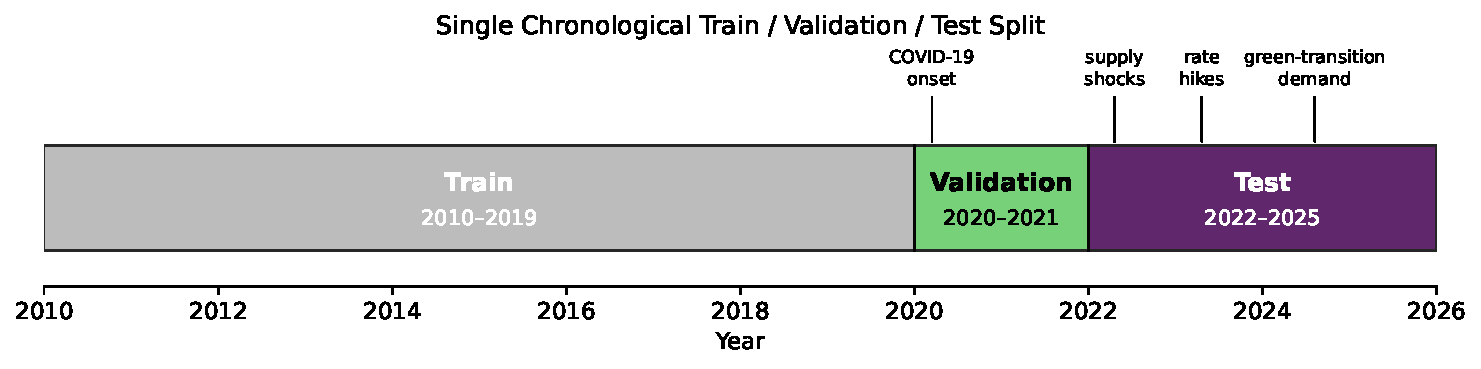
\includegraphics[width=\columnwidth]{../results/archive_paper1/figures/fig_data_split_timeline.pdf}
\caption{The single chronological train/validation/test split used throughout this paper, with the named regime events inside each window (Section~\ref{sec:limitations}). The split is not walked forward or resampled; this figure makes exactly what one split covers inspectable at a glance.}
\label{fig:datasplit}
\end{figure}

\subsection{Baselines}
\label{sec:baselines}

We compare VMD-MFGNN against six baselines: ARIMA, XGBoost, LSTM, Transformer, VMD-LSTM, and SimpleMTGNN, spanning econometric, machine-learning, deep-learning, decomposition-ensemble, and graph-based categories. All six run with standard, reasonable, hand-set configurations; none receive hyperparameter optimization (Section~\ref{sec:hpo}). ARIMA selects its $(p,d,q)$ order by AIC over a small grid per series; XGBoost uses 500 estimators, max depth 6, learning rate 0.05; LSTM, Transformer, VMD-LSTM, and SimpleMTGNN share a common training loop (hidden dimension 64, 2 recurrent/GNN layers where applicable, Adam at learning rate $10^{-3}$, up to 100 epochs with patience 20, lookback 60) and differ only in their architecture-specific layers, described next.

We are explicit that \textbf{``SimpleMTGNN'' and ``VMD-LSTM'' are our own simplified reimplementations of the design ideas in \citet{Wu2020mtgnn} and the VMD-LSTM literature respectively, not the original authors' code}, since neither published implementation is a plug-and-play fit for this study's $N=8$ variables and multi-horizon output. SimpleMTGNN keeps MTGNN's core idea --- a learned bilinear node-embedding adjacency feeding graph-based spatial mixing --- but omits the original's saturated top-k graph-learning layer, mix-hop propagation, dilated-inception temporal convolution, and skip connections, using instead a single linear spatial mix and two plain dilated causal convolutions; it should be read as a graph-learning baseline in the same architectural family as MTGNN, not a reproduction of its reported results. VMD-LSTM decomposes the input with the same VMD front end as VMD-MFGNN but feeds all $N=8$ variables jointly into a single per-mode LSTM (rather than one univariate LSTM per decomposed variable, the more common convention in the VMD-LSTM literature), so that it isolates the graph-construction step specifically as VMD-MFGNN's point of difference from a non-graph VMD+LSTM alternative, at the cost of not being a strict reproduction of any single prior VMD-LSTM paper's exact architecture. We flag this here because two of these baselines' cells are visibly pathological rather than merely weaker (SimpleMTGNN at $h=5$: RMSE 0.1345 against $\approx$0.04 for every other model, R$^2=-10.37$; VMD-LSTM at $h=1$: R$^2=-5.43$, Table~\ref{tab:r2}), and Section~\ref{sec:results-dm} revisits what this means for the significance comparisons that involve them.

\subsection{Hyperparameter Optimization}
\label{sec:hpo}

VMD-MFGNN, the proposed model, is tuned via a lightweight Optuna study (TPE sampler with a median pruner), searching hidden dimension $\in \{32,64,128\}$, number of attention heads $\in \{2,4,8\}$ (constrained so hidden dimension is divisible by the head count), learning rate (log-uniform, $10^{-4}$ to $10^{-2}$), dropout (uniform, 0.05 to 0.3), and number of GNN layers $\in \{1,2,3\}$, configured for up to 15 trials of 25 epochs each. Table~\ref{tab:hpo-space} tabulates this search space alongside the selected best trial. In the run reported in this paper, the study completed 10 of the configured 15 trials (5 \texttt{COMPLETE}, 5 \texttt{PRUNED} by the median pruner before completing their allotted epochs) before the search budget was exhausted; we report the true trial count rather than the configured one. The best trial (validation MSE $= 0.002051$) selected \textbf{hidden dimension $=128$, attention heads $=2$, learning rate $\approx 0.00153$, dropout $\approx 0.0616$, GNN layers $=1$}. This configuration is used for VMD-MFGNN throughout the main results (Table~\ref{tab:main}) and significance testing (Table~\ref{tab:dm}); it is \emph{not} used in the ablation study (Section~\ref{sec:ablation}), which fixes all variants, including its own \texttt{full\_model} row, at the untuned default configuration (Section~\ref{sec:impl}) instead. The six baselines are \emph{not} tuned; they run at standard/hardcoded settings. This asymmetry is a deliberate, disclosed methodological choice rather than an oversight: tuning all seven models under a full hyperparameter search would multiply compute cost roughly by the trial count and was judged infeasible within this project's compute and time budget, and tuning only the proposed model against standard baselines is common, defensible practice in comparison papers under such constraints, provided it is disclosed (Section~\ref{sec:limitations}). HPO results (best parameters and the full trial history, including pruned trials) are saved for reproducibility.

\begin{table}[t]
\centering
\caption{Main Optuna search space (Section~\ref{sec:hpo}) and the selected best trial (validation MSE $=0.002051$, 10 of 15 configured trials completed: 5 \texttt{COMPLETE}, 5 \texttt{PRUNED}).}
\label{tab:hpo-space}
\begin{tabular}{lll}
\toprule
Hyperparameter & Search space & Best trial \\
\midrule
hidden dim.\ $d_h$ & $\{32, 64, 128\}$ & 128 \\
attention heads $H$ & $\{2, 4, 8\}$ & 2 \\
learning rate & log-U$(10^{-4}, 10^{-2})$ & $\approx 0.00153$ \\
dropout & U$(0.05, 0.3)$ & $\approx 0.0616$ \\
GNN layers & $\{1, 2, 3\}$ & 1 \\
\bottomrule
\end{tabular}
\end{table}

\subsection{Ablation Studies}
\label{sec:ablation}

Six variants isolate the contribution of each architectural component, all trained at the untuned default configuration (Section~\ref{sec:impl}, Section~\ref{sec:complexity})---HPO (Section~\ref{sec:hpo}) is applied only to the main-table VMD-MFGNN, never to any ablation variant. Because this study uses a single chronological split rather than multiple walk-forward folds or multiple random seeds (Section~\ref{sec:limitations}), the ablation results below are reported as point estimates per horizon, without a paired significance test; a valid resampling unit (folds or seeds) does not exist for \emph{this} run to compute one. A separate five-seed repetition of the two variants that carry RQ1, run later at the tuned configuration and therefore not directly comparable to this table, does admit a paired test and is reported in Section~\ref{sec:robustness}.

Figure~\ref{fig:perband-vs-pooled} shows the architectural difference RQ1 asks about: variant (a), the full model of Figure~\ref{fig:architecture}, learns $K=5$ independent adjacency matrices and runs $K$ separate GAT+LSTM branches before fusing them; variant (c) pools the $K$ raw per-band VMD values for each variable through a learned linear projection (\texttt{nn.Linear(K,1)}) \emph{before} any GAT/LSTM encoding, then learns a single shared adjacency and runs one GAT+LSTM branch over that pooled scalar signal. We are explicit that this pools raw band \emph{values}, not learned band \emph{representations}, since the latter would imply pooling happens after per-band encoding rather than instead of it. The remaining five variants (the two capacity settings of b, d, and the two capacity settings of c) are described below.

\begin{figure}[t]
\centering
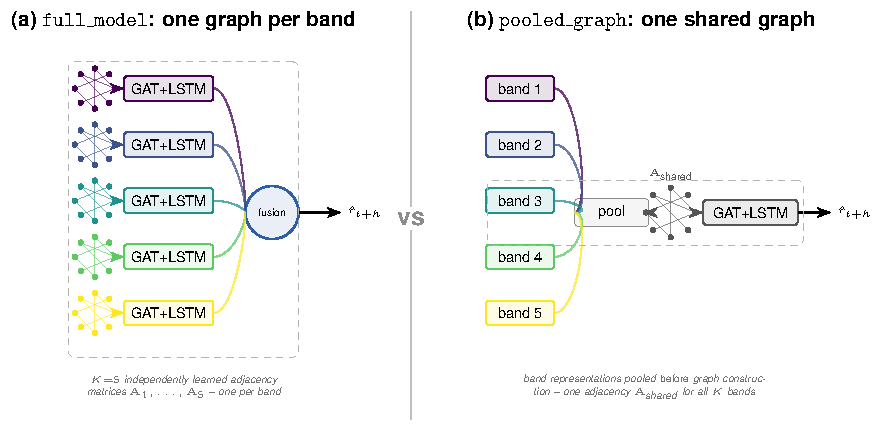
\includegraphics[width=\columnwidth]{figures/perband_vs_pooled.pdf}
\caption{The RQ1 comparison made visible: (a) \texttt{full\_model} builds a separate learned graph per frequency band; (c) \texttt{pooled\_graph} pools raw band \emph{values} (not learned representations) via a linear projection before constructing a single shared graph. Section~\ref{sec:collapse} shows that in the trained model, (a)'s five graphs collapse to a near-uniform adjacency indistinguishable from one another, which is why the ablation in Table~\ref{tab:ablation} does not show a clean advantage for (a) over (c).}
\label{fig:perband-vs-pooled}
\end{figure}

\begin{itemize}
    \item \textbf{(a) Full model}: VMD decomposition into $K=5$ bands, with a separate learned graph per band, at the untuned default configuration (393{,}476 parameters). This is a distinct trained instance from the HPO-tuned VMD-MFGNN reported in Table~\ref{tab:main} (1{,}461{,}124 parameters); see Section~\ref{sec:complexity}.
    \item \textbf{(b) No-VMD, raw price}: A genuine raw-price GAT+LSTM model with a single learned graph, using a dedicated raw-price dataloader that never touches VMD-decomposed input, reported at two capacity settings: \emph{matched-dim} (same hidden dimension as the full model, 88{,}836 params, $-$77.4\%) and \emph{matched-params} (hidden dimension increased to restore parameter count, 394{,}116 params, $+$0.16\%). This isolates the contribution of decomposition itself, independent of the per-band-graph question, at two different capacity assumptions.
    \item \textbf{(c) Pooled graph}: VMD decomposition retained, but the $K$ raw band \emph{values} are pooled (via a learned linear projection, before any GAT/LSTM encoding) into a single unified signal before a single graph is built over it, rather than building $K$ separate graphs. This is the ablation that most directly supports (or fails to support) the paper's central architectural claim against MBTI-Net-style pooling. Reported at two capacity settings: \emph{matched-dim} (84{,}618 params, $-$78.5\%) and \emph{matched-params} (397{,}586 params, $+$1.05\%). The matched-params setting lands within about 1\% of the full model's parameter count, so the (a)-vs-(c, matched-params) comparison is the cleanest available test of graph structure with capacity approximately controlled; the matched-dim setting is retained alongside it because it reflects the capacity a pooled architecture has \emph{by default} at equal hidden dimension, which is itself an architecturally meaningful comparison.
    \item \textbf{(d) Correlation graph}: The learned per-band adjacency is replaced with a fixed adjacency built from Pearson correlation between variables' band signals, thresholded at $|r|>0.3$ (392{,}196 params, $-$0.33\%, essentially parameter-matched to the full model). This isolates the contribution of end-to-end learned adjacency versus a fixed, precomputed graph, holding the per-band architecture fixed.
\end{itemize}

\subsection{Statistical Testing}

For the baseline comparison (VMD-MFGNN versus each of the six baselines, Section~\ref{sec:baselines}), we apply the Diebold-Mariano test \citep{DieboldMariano1995} to each pair of forecast error series, per horizon, testing whether VMD-MFGNN's forecast errors are significantly different from each baseline's. This test is applicable here because the same test-set forecasts, produced under the same single split, provide a valid paired sample of loss differentials over time. The test statistic is computed on the loss differential $d = e_{\text{VMD-MFGNN}}^2 - e_{\text{baseline}}^2$, divided by the square root of a heteroskedasticity-and-autocorrelation-consistent (HAC) variance estimate that sums $d$'s sample autocovariances at lags $1,\ldots,\text{horizon}-1$ with equal (rectangular-kernel) weight; this is a simpler, unweighted HAC-style correction, not the Bartlett-weighted kernel of the classical Newey-West estimator, and we describe it as such here to match the implementation exactly rather than name it Newey-West. Consequently a \emph{negative} DM statistic indicates VMD-MFGNN's squared error was lower (VMD-MFGNN better) and a \emph{positive} DM statistic indicates the baseline's squared error was lower (baseline better), and this sign convention is used without repeating it per cell in Table~\ref{tab:dm}. Because 24 DM tests are run (six baselines $\times$ four horizons), we additionally apply the Holm-Bonferroni step-down procedure to control the family-wise error rate across all 24 tests at $\alpha=0.05$, and report both the raw and Holm-corrected significance in Table~\ref{tab:dm} (Section~\ref{sec:results-dm}). An earlier version of this paper stated the DM test could not be applied to the ablation comparisons at all, reasoning from the absence of walk-forward folds or repeated seeds; that reasoning was itself mistaken, since the DM test's resampling unit is time within a single split (the same paired daily forecast-error series used for the baseline comparison above), not folds or seeds, and a single chronological split is exactly what the baseline comparison above also uses. The real obstacle was practical, not statistical: per-sample predictions were not archived for the ablation study's variants until a later fix (Section~\ref{sec:impl}) added this. With that fix, we now apply the DM test to this paper's single most important ablation comparison --- \texttt{full\_model} versus \texttt{pooled\_graph\_matched\_params}, the capacity-matched pairing that most directly targets RQ1 --- and report it in Section~\ref{sec:ablation-results} alongside Table~\ref{tab:ablation}. We did not extend it to the remaining ablation pairs (no-VMD and correlation-graph variants, or the matched-dim capacity setting), since RQ1 is the comparison this paper's central claim depends on and we did not want to run a large additional battery of tests without a correction plan to match; this remains a direction for future work rather than a claimed impossibility. Where seeds \emph{are} available --- the five-seed repetition of the two RQ1 variants at the tuned configuration, Section~\ref{sec:robustness} --- we separately report paired $t$- and Wilcoxon signed-rank tests over seeds, which is complementary evidence at a different configuration, not a substitute for the DM test above.

\subsection{Evaluation Metrics}

RMSE, MAE, and Directional Accuracy (DA) are reported for the main comparison and the ablations, per horizon. DA is computed as $\text{mean}(\text{sign}(r_{t+h}) = \text{sign}(\hat r_{t+h})) \times 100$; we state the zero-return convention this implies explicitly, since it is only ever otherwise visible deep inside a Section~\ref{sec:results} discussion. NumPy's \texttt{sign} returns exactly $0$ for an exactly-zero input, so a true return of exactly zero counts as a directional hit only on the practically-never-occurring event that the model's continuous-valued prediction is also exactly $0.0$; in every other case, including every ordinary nonzero prediction, an exactly-zero true return counts as a miss. This is a fixed, mechanical consequence of the sign-comparison formula, not a design choice made specifically for this paper, and it is applied identically to every model and every table in this paper.

\subsection{Implementation Details}
\label{sec:impl}

VMD-MFGNN and all baselines are implemented in PyTorch with PyTorch Geometric for the GAT layers. Default (pre-HPO) architecture hyperparameters are: hidden dimension 64, 4 attention heads, 2 GNN layers, 2 LSTM layers, embedding dimension $d=16$ for the bilinear graph embeddings $\mathbf{E}^{(1)}_k,\mathbf{E}^{(2)}_k$ of Eq.~\ref{eq:graph} (fixed, not part of the HPO search space of Section~\ref{sec:hpo}, so it is identical across the default and HPO-tuned configurations), dropout 0.1, lookback window $L=60$ trading days; training uses batch size 32, the Adam optimizer with learning rate $10^{-3}$ and coupled $L_2$ weight decay $10^{-5}$ applied uniformly to all parameters (including the graph-embedding parameters discussed in Section~\ref{sec:collapse}), and early stopping with patience 20 (maximum budget 200 epochs), seed 42 throughout. Best-validation-loss checkpoint selection was used for all reported models, with model weights saved to disk so that training can resume from a checkpoint rather than restart from scratch. Every result reported in Table~\ref{tab:main}, Table~\ref{tab:dm}, Table~\ref{tab:ablation}, and Table~\ref{tab:confound-tuned} uses a checkpoint-selection floor \texttt{min\_epochs}$=0$, i.e.\ the historical, unconstrained behavior in which the best-validation checkpoint is eligible from epoch 0; we flag this explicitly because a later diagnostic (Section~\ref{sec:robustness}) found this can, in rare cases, allow an effectively untrained checkpoint (best-validation loss reached in the first few epochs and never subsequently improved upon) to be reported as a trained model's result. The confirmed instances of this failure mode in this paper are in the ablation study and graph-fix experiment (Sections~\ref{sec:ablation} and~\ref{sec:graphfix}), which we discuss there and, where a re-run with a corrective floor is available, report separately. We did not archive a per-model effective-epoch count for this section's tables (Table~\ref{tab:main}, Table~\ref{tab:dm}) at the time they were run, so we cannot rule this out for those specific numbers with the same direct evidence used elsewhere in this paper, and note it here as an unresolved reproducibility gap rather than claim a verification that was not actually performed.

\textbf{Environment.} Training was run on Google Colab with a single NVIDIA T4 GPU (paid compute-unit tier, not the free tier). Package versions are pinned only as lower bounds in the project's \texttt{requirements.txt} (PyTorch $\geq$2.0, PyTorch Geometric $\geq$2.4, Optuna $\geq$3.0); we did not additionally freeze exact resolved versions for this run, which we note here as a reproducibility gap rather than omit silently. Given the dataset scale ($N=8$ series, $\sim$4{,}000 trading days), a single VMD-MFGNN training run completes in low single-digit minutes on this hardware; we did not instrument and log per-run wall-clock time precisely enough to report a more exact figure for every one of this paper's model/variant combinations, and state that limitation explicitly rather than back-fill an estimate.

%% ============================================================
\section{Results and Discussion}
\label{sec:results}

All numbers below are computed on the test split (2022--2025) and read directly from the training and evaluation pipeline's saved output artifacts, with no recomputation or adjustment beyond the naive-baseline row, the Holm-Bonferroni correction, and the ablation-table cross-checks described explicitly where they appear.

\subsection{Main Results, Including a Naive Baseline}
\label{sec:main-results}

Table~\ref{tab:main} reports RMSE, MAE, and Directional Accuracy (DA) for VMD-MFGNN and the six baselines, across all four forecast horizons, together with a trivial \textbf{zero-forecast (random-walk) baseline} that predicts $\hat r_{t+h}=0$ for every sample. We add this row because it is the single most important context for reading the rest of this table, and because omitting it, as much of the decomposition-ensemble and GNN-for-finance literature does, risks presenting a ranking among models that all fail a more basic test. For a zero forecast, RMSE reduces to the standard deviation of the true returns and MAE to their mean absolute value, computed directly from the saved test-set target arrays (identical across all seven models since they share one test set).

\begin{table*}[!tb]
\centering
\caption{Forecasting performance comparison across four horizons, test split (2022--2025). Best result per column shown in \textbf{bold}. VMD-MFGNN is the HPO-tuned model (Section~\ref{sec:hpo}); the six baselines are untuned. $^{\ddagger}$Transformer's $h=5$ DA is a confirmed base-rate artifact: its predictions are 100\% positive-sign and this DA value exactly equals the test period's up-day frequency, not a measurement of directional skill; see the sign-concentration diagnostic in Section~\ref{sec:constantforecast}.}
\label{tab:main}
\resizebox{\textwidth}{!}{%
\begin{tabular}{l cccc cccc cccc}
\toprule
& \multicolumn{4}{c}{RMSE} & \multicolumn{4}{c}{MAE} & \multicolumn{4}{c}{DA (\%)} \\
\cmidrule(lr){2-5} \cmidrule(lr){6-9} \cmidrule(lr){10-13}
Model & $h$=1 & $h$=5 & $h$=10 & $h$=22 & $h$=1 & $h$=5 & $h$=10 & $h$=22 & $h$=1 & $h$=5 & $h$=10 & $h$=22 \\
\midrule
ARIMA           & 0.0182 & 0.0403 & 0.0555 & 0.0760 & 0.0122 & 0.0281 & 0.0399 & 0.0572 & 49.4 & 48.7 & 49.3 & \textbf{49.9} \\
XGBoost         & 0.0180 & 0.0399 & \textbf{0.0551} & 0.0765 & 0.0121 & 0.0279 & 0.0397 & 0.0578 & 46.8 & 51.2 & 48.8 & 42.7 \\
LSTM            & 0.0193 & 0.0416 & 0.0606 & 0.0834 & 0.0136 & 0.0288 & 0.0468 & 0.0675 & 48.7 & \textbf{53.7} & 45.2 & 45.9 \\
Transformer     & 0.0231 & 0.0493 & 0.0575 & 0.1053 & 0.0177 & 0.0357 & 0.0420 & 0.0870 & 51.9 & 53.0$^{\ddagger}$ & \textbf{52.7} & 44.7 \\
VMD-LSTM        & 0.0453 & 0.0458 & 0.0637 & 0.0961 & 0.0366 & 0.0334 & 0.0474 & 0.0765 & 48.9 & 49.5 & 51.5 & 48.9 \\
SimpleMTGNN     & 0.0187 & 0.1345 & 0.0667 & 0.0977 & 0.0130 & 0.1087 & 0.0537 & 0.0782 & 48.3 & 47.3 & 44.5 & 47.8 \\
VMD-MFGNN & 0.0184 & \textbf{0.0398} & 0.0552 & 0.0785 & 0.0125 & 0.0282 & 0.0407 & 0.0608 & \textbf{52.5} & 50.8 & 47.7 & 47.1 \\
\midrule
\textbf{Zero-forecast (naive)} & \textbf{0.0179} & 0.0399 & 0.0552 & \textbf{0.0759} & \textbf{0.0120} & \textbf{0.0279} & \textbf{0.0397} & \textbf{0.0571} & --- & --- & --- & --- \\
\midrule
Unconditional up-day freq.\ (\%) & \multicolumn{4}{c}{} & \multicolumn{4}{c}{} & 51.0 & 53.0 & 55.4 & 55.3 \\
\bottomrule
\end{tabular}%
}
\end{table*}
\FloatBarrier

Table~\ref{tab:main} makes the central finding of this paper visible in one place: \textbf{the naive zero-forecast baseline wins MAE at all four horizons and RMSE at two of four horizons ($h=1$ and $h=22$), against every one of the seven fitted models, including VMD-MFGNN.} No model beats it on MAE anywhere in the table; VMD-MFGNN and XGBoost each beat it on RMSE at one horizon ($h=5$ and $h=10$ respectively), and nowhere else does any model do better than predicting zero return. All seven models' $R^2$ values are negative or approximately zero on this test split, consistent with none of them explaining variance beyond what a constant forecast already captures; Table~\ref{tab:r2} reports them in full, since RQ0 is load-bearing enough to this paper's framing that we do not leave its supporting statistic as an unlabeled aside.

\begin{table}[t]
\centering
\caption{$R^2$ by model and horizon, test split (2022--2025), computed identically to RMSE/MAE (Table~\ref{tab:main}) from the same saved prediction arrays. Best (least negative, or positive) per column shown in \textbf{bold}. All values are negative or approximately zero: no model explains test-set variance beyond a constant (zero) forecast.}
\label{tab:r2}
\begin{tabular}{lrrrr}
\toprule
Model & $h$=1 & $h$=5 & $h$=10 & $h$=22 \\
\midrule
ARIMA & $-$0.0396 & $-$0.0196 & $-$0.0120 & \textbf{$-$0.0071} \\
XGBoost & $-$0.0121 & $-$0.0009 & \textbf{0.0014} & $-$0.0198 \\
LSTM & $-$0.1638 & $-$0.0856 & $-$0.2064 & $-$0.2120 \\
Transformer & $-$0.6752 & $-$0.5307 & $-$0.0879 & $-$0.9302 \\
VMD-LSTM & $-$5.4306 & $-$0.3158 & $-$0.3349 & $-$0.6086 \\
SimpleMTGNN & $-$0.0930 & $-$10.3659 & $-$0.4616 & $-$0.6640 \\
VMD-MFGNN & $-$0.0651 & \textbf{0.0041} & $-$0.0030 & $-$0.0747 \\
\bottomrule
\end{tabular}
\end{table}

RQ0's naive-baseline comparison above is a raw MAE/RMSE ranking, not a significance test; we close that gap with a direct Diebold-Mariano test of VMD-MFGNN against the same zero-forecast baseline, computed from the same saved prediction arrays as Table~\ref{tab:dm} (Section~\ref{sec:experiments}), using the identical sign convention (positive DM favors the baseline, here the naive zero-forecast). At $h=1$, VMD-MFGNN is significantly worse than the naive baseline (DM$=3.40$, $p=0.0007$, surviving Holm-Bonferroni correction across these four tests at $\alpha=0.05$); at $h=5,10,22$ the difference is not significant (DM$=-0.14,\ p=0.89$; DM$=0.04,\ p=0.97$; DM$=0.92,\ p=0.36$, respectively). This sharpens rather than merely restates the MAE/RMSE picture above: VMD-MFGNN is not merely failing to beat the naive baseline by some margin at $h=1$, it is significantly worse than it, and at the other three horizons the two are statistically indistinguishable rather than VMD-MFGNN being non-significantly close to a win. We read this as the more precise and more honest form of RQ0's answer, and use it in place of the raw ranking wherever this paper draws a conclusion from RQ0 that depends on significance rather than only direction.

DA tells a related story once read against the correct null: the relevant baseline for DA is not 50\% but the test period's own unconditional up-day frequency, which is 51.0\%, 53.0\%, 55.4\%, and 55.3\% at $h=1,5,10,22$ respectively (bottom row) --- itself a symptom of the strong upward drift copper exhibited over 2022--2025. The complementary down-day frequencies are 48.37\%, 46.95\%, 44.21\%, and 44.72\% (they do not sum to exactly 100\% with the up-day figures because a small number of test days record an exactly zero return); we state them explicitly because the base-rate-identity checks reported below and in Section~\ref{sec:ablation-results} are made against whichever of the two frequencies matches the sign a degenerate model emits, and a reader cannot otherwise verify those flags from the table alone. VMD-MFGNN's headline $h=1$ DA of 52.5\% is only 1.5 percentage points above that null, and at $h=10,22$ no model in this table, including VMD-MFGNN, exceeds the unconditional up-day frequency at all; at $h=5$ one model, LSTM (53.7\% vs.\ the 53.0\% null), marginally does, though LSTM's own sign concentration at nearby horizons (discussed below) argues against reading this half-point margin as demonstrated directional skill. We read this table as showing that this study's seven fitted models, including the proposed one, are best understood as a ranking among approaches that do not clearly outperform doing nothing, rather than as a demonstration that any of them, including VMD-MFGNN, has found exploitable structure in copper returns at this data scale. Section~\ref{sec:results-dm} still reports pairwise significance among the seven fitted models, since that question --- do these models differ meaningfully from one another --- is separate from, and does not resolve, the more basic question this section answers in the negative. We applied this paper's own base-rate-identity check (Section~\ref{sec:constantforecast}) to every cell of this table directly, loading all 28 saved prediction arrays and checking both the fraction of predictions sharing the majority sign and whether DA exactly equals the test period's class frequency: exactly one cell qualifies, Transformer at $h=5$ (100\% positive-sign predictions, DA=53.05\% identical to the up-day frequency to four decimal places, marked $^{\ddagger}$ above). Transformer's $h=22$ DA (44.72\%) also happens to numerically equal the down-day frequency at that horizon, but this is a coincidental count match, not the same artifact: only 89.4\% of its predictions are negative-sign and its prediction standard deviation is a healthy fraction of the true-return standard deviation, so we do not flag it. No other cell in this table shows the strict, exact-identity signature. We separately report a softer, non-exact version of the same check --- majority-sign concentration $\geq 90\%$ without requiring DA to match the class frequency exactly --- since a model can be highly sign-concentrated without landing on the identity by coincidence: seven further cells clear this looser bar (LSTM at $h=10$, 97.8\% negative-sign; LSTM at $h=22$, 98.2\% negative-sign; SimpleMTGNN at $h=5$, 99.7\% negative-sign; SimpleMTGNN at $h=10$, 99.7\% negative-sign; SimpleMTGNN at $h=22$, 96.3\% negative-sign; VMD-LSTM at $h=1$, 94.6\% negative-sign; XGBoost at $h=5$, 90.5\% positive-sign). These are not base-rate-identity matches and we do not mark them with $^{\ddagger}$ in Table~\ref{tab:main}, but their dispersion ratios (predicted-return std.\ over true-return std.) split into two distinct patterns worth distinguishing: XGBoost at $h=5$ (ratio 0.019) and LSTM at $h=10$ (ratio 0.163) show the low dispersion characteristic of a near-constant-output degeneracy, just without landing on the exact class frequency by chance; SimpleMTGNN at $h=5$ (ratio 1.869) and VMD-LSTM at $h=1$ (ratio 1.363) are not, since a near-constant predictor cannot simultaneously reproduce more dispersion than the true series --- these two are genuinely, if unhelpfully, one-sided rather than degenerate. We deliberately do not compare either pattern to the flagged Transformer $h=5$ cell here: Section~\ref{sec:constantforecast} shows that cell's own dispersion ratio (0.42) is healthy, unremarkable output despite its 100\% sign concentration and exact base-rate match, which is precisely why a dispersion check alone would not have caught it and the sign/exact-match check was needed in the first place. Sign concentration and low dispersion are related but distinct signatures, and we do not conflate them across this paragraph. We report this distinction for completeness and transparency rather than as a basis for any additional claim in this paper. We applied the same $\geq 90\%$ check to VMD-MFGNN itself, not only to the baselines: its majority-sign fraction is 81.2\% ($h=1$), 60.4\% ($h=5$), 81.6\% ($h=10$), and 85.1\% ($h=22$), so the proposed model stays below this looser bar at every horizon and is not merely exempt because we did not look.

Figure~\ref{fig:comparison} shows the seven-model comparison graphically (grouped bar charts of RMSE, MAE, and DA by model and horizon; the naive baseline is not part of this bar chart, which mirrors the pipeline's model-comparison output). No model's saved evaluation record carried an error flag, so all seven models are represented in both Table~\ref{tab:main} and Figure~\ref{fig:comparison}.

\begin{figure*}[!tb]
\centering
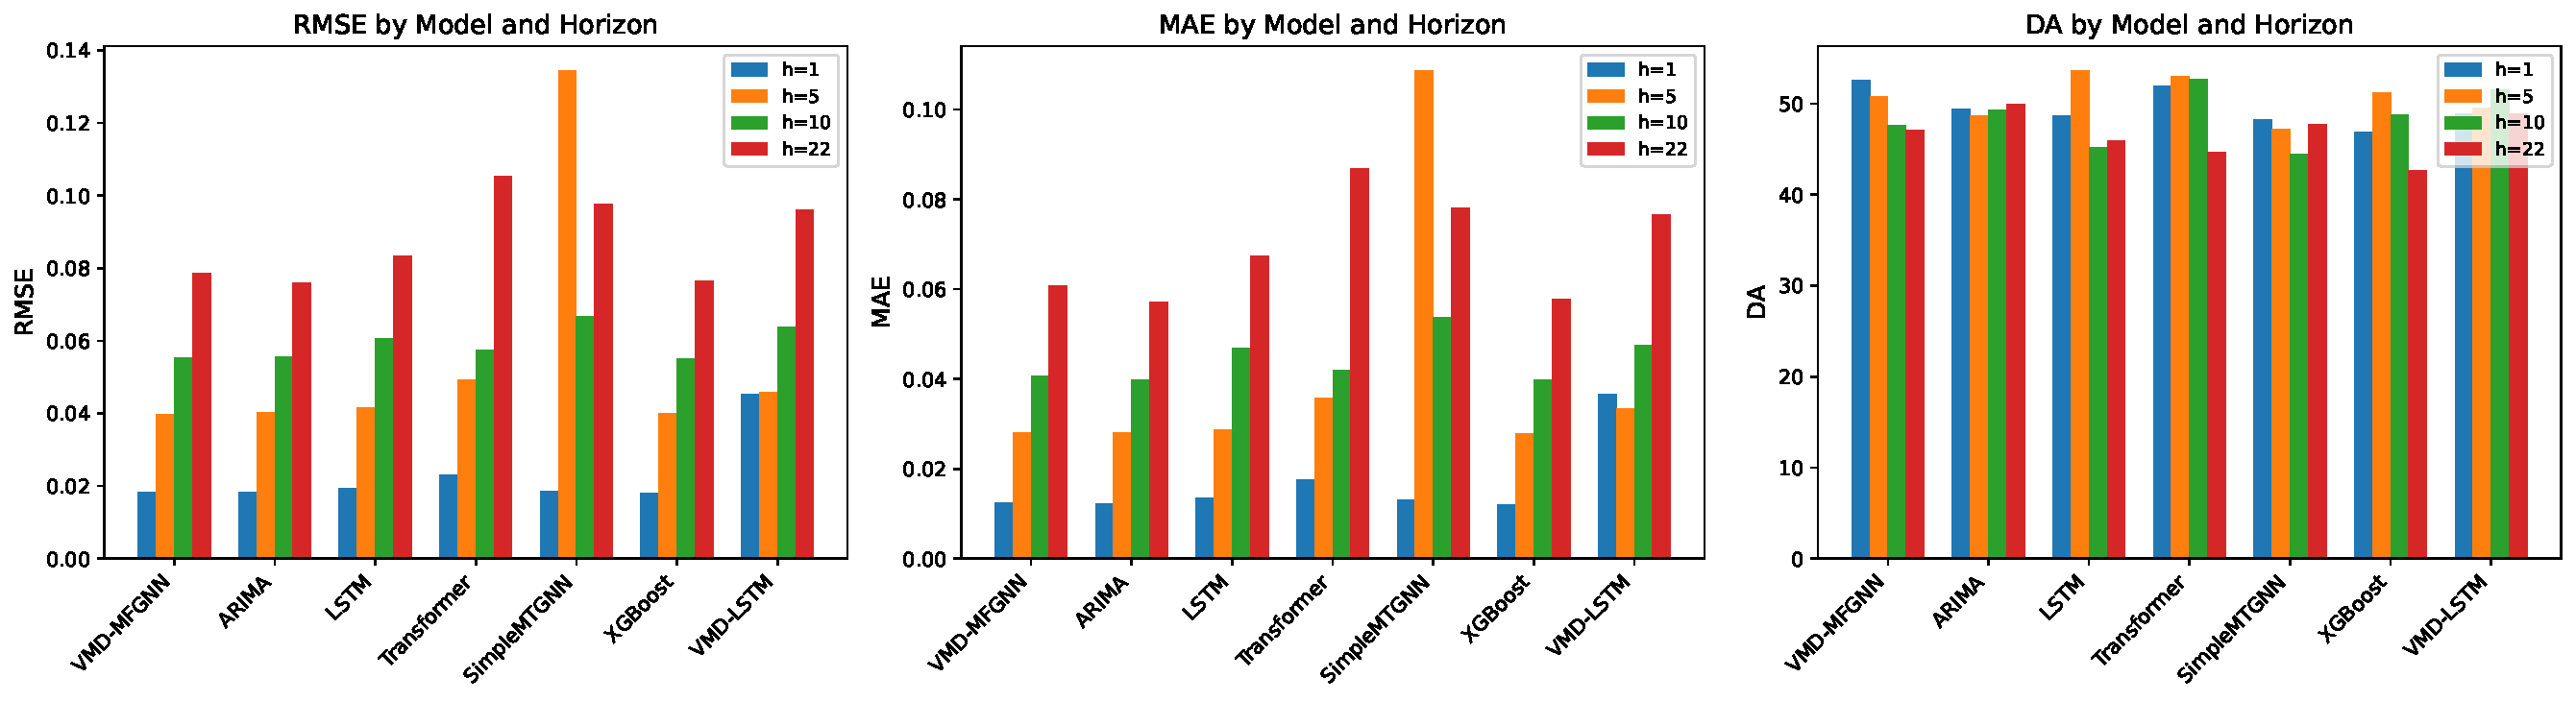
\includegraphics[width=\textwidth]{../results/archive_paper1/figures/fig4_model_comparison.pdf}
\caption{RMSE, MAE, and Directional Accuracy by model and horizon, for VMD-MFGNN and the six baselines.}
\label{fig:comparison}
\end{figure*}

\subsection{Statistical Significance versus Baselines}
\label{sec:results-dm}

Table~\ref{tab:dm} reports the Diebold-Mariano statistic and $p$-value for VMD-MFGNN's forecast errors against each of the six baselines, per horizon (Section~\ref{sec:experiments}). Recall the sign convention (Section~\ref{sec:experiments}): the DM statistic is computed as $e_{\text{VMD-MFGNN}}^2 - e_{\text{baseline}}^2$, so a \emph{negative} DM statistic means VMD-MFGNN had the lower squared error (VMD-MFGNN better), and a \emph{positive} DM statistic means the baseline had the lower squared error (baseline better); boldface marks $p<0.05$. This test is applied only to the baseline comparison, not to the ablation table (Table~\ref{tab:ablation}); see Section~\ref{sec:limitations}. All 24 test entries are finite (no degenerate $\mathrm{var}_d \le 0$ cases were observed at full data scale).

\begin{table*}[!t]
\centering
\caption{Diebold-Mariano test: VMD-MFGNN versus each baseline, per horizon. Negative DM statistic favors VMD-MFGNN; positive favors the baseline. Bold $p$-values indicate significance at $\alpha=0.05$ uncorrected; $^{\dagger}$ marks the subset that remains significant after Holm-Bonferroni correction across all 24 tests.}
\label{tab:dm}
\begin{tabular}{l cccc cccc}
\toprule
& \multicolumn{4}{c}{DM statistic} & \multicolumn{4}{c}{$p$-value} \\
\cmidrule(lr){2-5} \cmidrule(lr){6-9}
vs.\ Baseline & $h$=1 & $h$=5 & $h$=10 & $h$=22 & $h$=1 & $h$=5 & $h$=10 & $h$=22 \\
\midrule
ARIMA        & 1.111 & $-$0.644 & $-$0.171 & 0.867 & 0.267 & 0.520 & 0.864 & 0.386 \\
XGBoost      & 2.459 & $-$0.150 & 0.092 & 0.781 & \textbf{0.014} & 0.880 & 0.927 & 0.435 \\
LSTM         & $-$2.522 & $-$1.012 & $-$3.595 & $-$1.489 & \textbf{0.012} & 0.311 & \textbf{0.0003}$^{\dagger}$ & 0.137 \\
Transformer  & $-$11.219 & $-$3.319 & $-$1.101 & $-$3.734 & \textbf{$<$0.001}$^{\dagger}$ & \textbf{0.001}$^{\dagger}$ & 0.271 & \textbf{$<$0.001}$^{\dagger}$ \\
VMD-LSTM     & $-$16.777 & $-$3.464 & $-$2.696 & $-$2.217 & \textbf{$<$0.001}$^{\dagger}$ & \textbf{0.001}$^{\dagger}$ & \textbf{0.007} & \textbf{0.027} \\
SimpleMTGNN  & $-$0.860 & $-$7.872 & $-$4.050 & $-$2.304 & 0.390 & \textbf{$<$0.001}$^{\dagger}$ & \textbf{$<$0.001}$^{\dagger}$ & \textbf{0.021} \\
\bottomrule
\end{tabular}
\end{table*}

\FloatBarrier

At the uncorrected $\alpha=0.05$ level, VMD-MFGNN attains a statistically significant advantage (negative DM statistic, $p<0.05$) over VMD-LSTM at all four horizons, over Transformer at three of four horizons ($h=1,5,22$), over SimpleMTGNN at three of four horizons ($h=5,10,22$), and over LSTM at two of four horizons ($h=1,10$; two of four is not a majority, and we state it as two of four rather than describing it loosely as most horizons)---12 of 24 comparisons favor VMD-MFGNN significantly, plus one significant result in the opposite direction (XGBoost at $h=1$, below), for 13 of 24 raw-significant cells in total. Because 24 tests were run without correction, we also apply the Holm-Bonferroni step-down procedure at family-wise $\alpha=0.05$ (Section~\ref{sec:experiments}); this reduces the significant count from 12 (favoring VMD-MFGNN) to 8, marked $^{\dagger}$ in Table~\ref{tab:dm}, and, notably, removes VMD-MFGNN's only significant loss: XGBoost's $h=1$ advantage ($p=0.014$ raw) does not survive correction (Holm threshold at that step is $0.00357$). After correction, VMD-MFGNN's remaining significant advantages are concentrated at shorter-to-medium horizons against Transformer ($h=1,5,22$), VMD-LSTM ($h=1,5$), SimpleMTGNN ($h=5,10$), and LSTM ($h=10$ only). Against ARIMA, no horizon reaches significance in either direction, corrected or not. Against XGBoost, no horizon is significant after correction; we still report the raw, uncorrected $h=1$ result ($p=0.014$, XGBoost lower squared error) in the table for transparency, but do not carry it forward as a supported claim once multiple testing is accounted for. VMD-MFGNN's significant edge in this study, corrected or uncorrected, is concentrated against the deep-learning baselines (LSTM, Transformer, VMD-LSTM, SimpleMTGNN), not against the two simpler, non-deep-learning baselines (ARIMA, XGBoost). We flag one further qualification specific to \emph{which} deep-learning cells this edge comes from: of the 8 Holm-surviving wins, 5 (Transformer $h=5$; VMD-LSTM $h=1$; SimpleMTGNN $h=5,10$; LSTM $h=10$) are against cells this paper's own sign-concentration diagnostic (Section~\ref{sec:main-results}) separately flags as a confirmed base-rate artifact or $\geq90\%$ sign-concentrated, and two of those five (SimpleMTGNN, VMD-LSTM) are baselines Section~\ref{sec:baselines} discloses as simplified reimplementations with visibly pathological error at exactly those horizons. Only 3 of the 8 (Transformer $h=1,22$; VMD-LSTM $h=5$) are wins against baseline cells free of either caveat. A win against a degenerate or pathological opponent is not evidence VMD-MFGNN itself is exploiting real structure, so we read this comparison as weaker support for RQ3 than the raw 8-of-24 count on its own would suggest, and we carry this qualification into the RQ3 answer in Section~\ref{sec:discussion}. Section~\ref{sec:main-results}'s naive-baseline comparison remains the more important context for interpreting any of these significant differences: a significant DM result establishes that two models' squared errors differ, not that either model is exploiting real structure in copper returns, which Table~\ref{tab:main} indicates neither is doing relative to a zero forecast.

\subsection{Ablation Study}
\label{sec:ablation-results}

Table~\ref{tab:ablation} reports RMSE, MAE, and DA per horizon for the six ablation variants defined in Section~\ref{sec:ablation}, all trained at the untuned default configuration. The table itself carries no significance column, since a full $\binom{6}{2}$ pairwise significance battery across all variants was out of scope for this study (Section~\ref{sec:experiments} explains why); a Diebold-Mariano test for this paper's single central ablation comparison (\texttt{full\_model} vs.\ \texttt{pooled\_graph\_matched\_params}) is reported in prose directly below the table. Reported parameter counts are exact, read from the trained checkpoints (Section~\ref{sec:complexity}), not estimated. Table~\ref{tab:ablation-config} consolidates each variant's architecture and exact parameter count in one place, since the matched-dim/matched-params distinction is otherwise easy to lose track of across running prose.

\begin{table}[t]
\centering
\caption{Ablation-variant configurations. All variants share the untuned default attention-head count (4) and GNN-layer count (2, Section~\ref{sec:impl}); only VMD, graph type, and hidden dimension $d_h$ vary. Parameter counts read directly from each variant's trained checkpoint state dict.}
\label{tab:ablation-config}
\resizebox{\columnwidth}{!}{%
\begin{tabular}{lccccc}
\toprule
Variant & VMD? & Graph & $d_h$ & Params & $\Delta$\% \\
\midrule
(a) full\_model & \checkmark & per-band ($K{=}5$) & 64 & 393{,}476 & --- \\
(b) no\_vmd\_matched\_dim & --- & single & 64 & 88{,}836 & $-$77.4\% \\
(b) no\_vmd\_matched\_params & --- & single & 136 & 394{,}116 & $+$0.16\% \\
(c) pooled\_matched\_dim & \checkmark & pooled (single) & 64 & 84{,}618 & $-$78.5\% \\
(c) pooled\_matched\_params & \checkmark & pooled (single) & 140 & 397{,}586 & $+$1.05\% \\
(d) correlation\_graph & \checkmark & per-band, fixed (not learned) & 64 & 392{,}196 & $-$0.33\% \\
\bottomrule
\end{tabular}%
}
\end{table}

\begin{table*}[!t]
\centering
\caption{Ablation study results, all four horizons, test split, from the corrected re-run with the \texttt{min\_epochs}=10 checkpoint-selection floor (Section~\ref{sec:impl}) applied to every variant, superseding an earlier run whose checkpoint-selection bug is described in Section~\ref{sec:limitations}. All variants trained at the untuned default configuration; this is a different, smaller VMD-MFGNN instance than the HPO-tuned model in Table~\ref{tab:main}. Best result per column shown in \textbf{bold}, computed from full, unrounded precision (so two cells can display the same rounded value while only one is bolded). $^{\ddagger}$Marks DA values \emph{confirmed} as base-rate artifacts by both criteria this paper uses (Section~\ref{sec:constantforecast}): majority-sign concentration $\geq90\%$ and an exact match, to the precision shown, of the test period's class frequency for that horizon --- verified directly from this run's newly-archived per-sample predictions, not inferred from the DA value alone. Confirmed cells are excluded from best-in-column eligibility. A Diebold-Mariano significance test for the paper's central RQ1 comparison (row (a) vs.\ the capacity-matched row (c)) is reported in the text below the table, now possible for the first time since this run is the first to archive per-sample ablation predictions.}
\label{tab:ablation}
\resizebox{\textwidth}{!}{%
\begin{tabular}{l cccc cccc cccc}
\toprule
& \multicolumn{4}{c}{RMSE} & \multicolumn{4}{c}{MAE} & \multicolumn{4}{c}{DA (\%)} \\
\cmidrule(lr){2-5} \cmidrule(lr){6-9} \cmidrule(lr){10-13}
Variant & $h$=1 & $h$=5 & $h$=10 & $h$=22 & $h$=1 & $h$=5 & $h$=10 & $h$=22 & $h$=1 & $h$=5 & $h$=10 & $h$=22 \\
\midrule
(a) Full model (393{,}476 params) & 0.0183 & 0.0403 & 0.0563 & 0.0787 & 0.0125 & 0.0290 & 0.0420 & 0.0617 & 48.6 & 49.7 & 46.5 & \textbf{48.2} \\
(b) No-VMD, matched-dim (88{,}836) & \textbf{0.0179} & 0.0406 & 0.0572 & 0.0829 & \textbf{0.0119} & 0.0293 & 0.0434 & 0.0660 & \textbf{50.9} & \textbf{49.9} & 44.2$^{\ddagger}$ & 44.7$^{\ddagger}$ \\
(b) No-VMD, matched-params (394{,}116) & 0.0179 & 0.0412 & 0.0570 & 0.0790 & 0.0120 & 0.0295 & 0.0427 & 0.0614 & 48.4$^{\ddagger}$ & 47.0$^{\ddagger}$ & 44.2$^{\ddagger}$ & 44.7$^{\ddagger}$ \\
(c) Pooled graph, matched-dim (84{,}618) & 0.0318 & 0.0411 & 0.0578 & 0.0829 & 0.0254 & 0.0296 & 0.0429 & 0.0660 & 49.8 & 47.0$^{\ddagger}$ & 43.5 & 44.7$^{\ddagger}$ \\
(c) Pooled graph, matched-params (397{,}586) & 0.0180 & \textbf{0.0400} & 0.0561 & 0.0760 & 0.0120 & \textbf{0.0280} & 0.0412 & 0.0578 & 50.6 & 48.1 & 44.6 & 47.2 \\
(d) Correlation graph (392{,}196) & 0.0183 & 0.0402 & \textbf{0.0551} & \textbf{0.0754} & 0.0125 & 0.0288 & \textbf{0.0406} & \textbf{0.0577} & 48.8 & 48.2 & \textbf{49.9} & 46.6 \\
\bottomrule
\end{tabular}%
}
\end{table*}

Figure~\ref{fig:ablation} shows the same comparison graphically.

\begin{figure*}[!t]
\centering
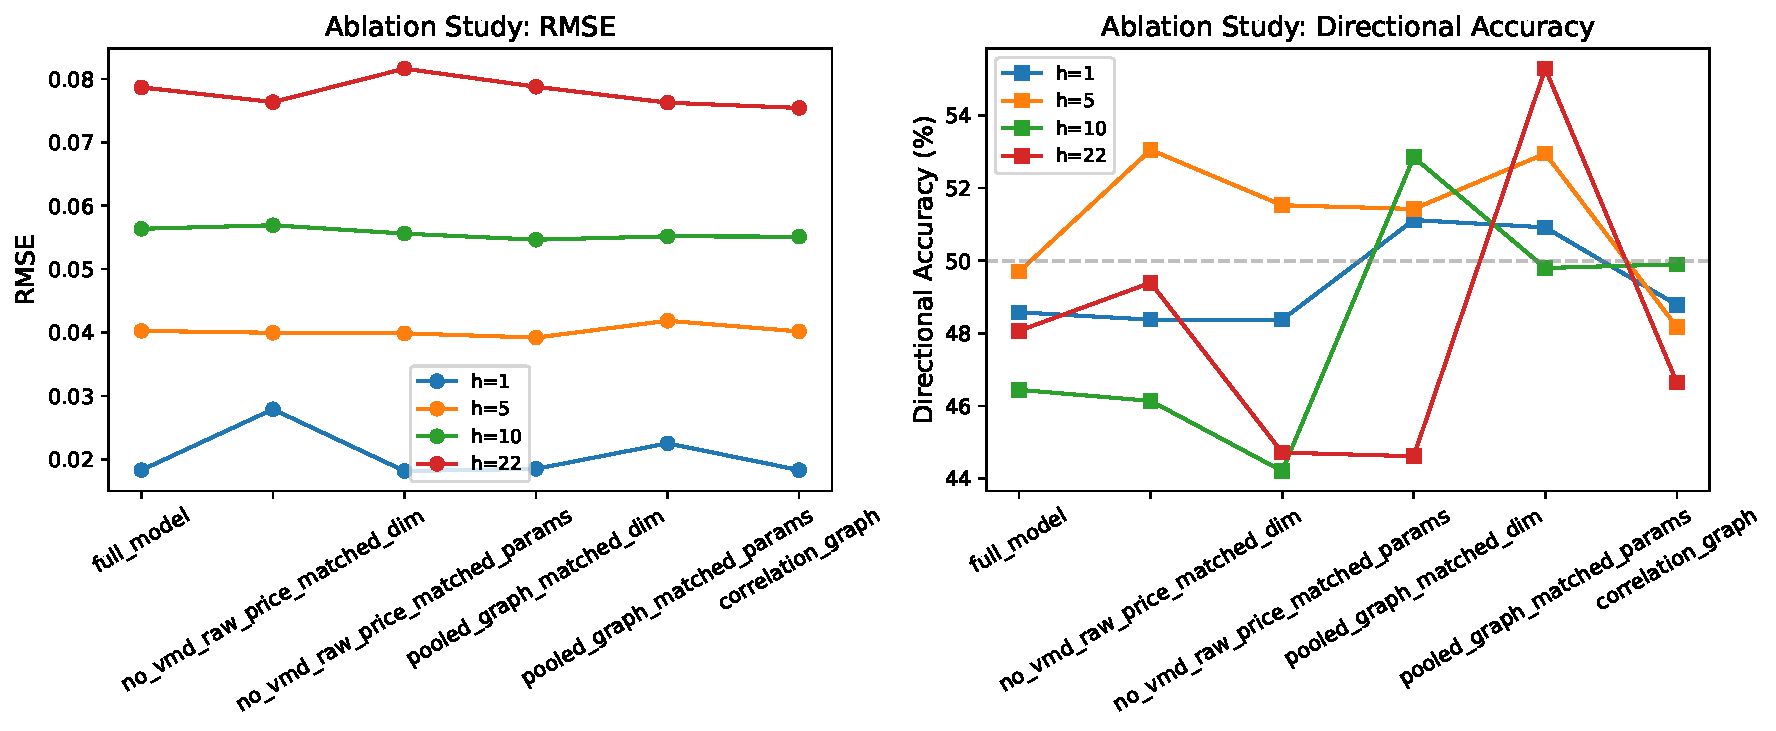
\includegraphics[width=\textwidth]{../results/archive_paper1/figures/fig5_ablation.pdf}
\caption{RMSE and Directional Accuracy across the six ablation variants, one line per horizon.}
\label{fig:ablation}
\end{figure*}

\textbf{This table does not support the paper's central architectural claim, and we report that plainly, stated precisely rather than more strongly than the numbers allow.} This is the corrected re-run: every variant now uses the \texttt{min\_epochs}=10 checkpoint-selection floor (Section~\ref{sec:impl}), and per-sample predictions were archived for the first time, so both the numbers and the sign-concentration flags below are independently verified rather than inferred. The precise claim is: row (a), the per-band full model, attains the \emph{best-of-six} value in exactly one of twelve RMSE/MAE/DA columns --- DA at $h=22$ (48.2\%), a clean win not subject to any sign-concentration or base-rate-identity flag. Against \texttt{pooled\_graph\_matched\_params} (397{,}586 vs.\ 393{,}476 params, $+$1.05\%, the comparison most directly targeting RQ1 with capacity approximately controlled), the full model now loses RMSE and MAE at \emph{all four} horizons ($h=1,5,10,22$), reversing what an earlier, since-corrected run of this same comparison reported; a Diebold-Mariano test on this exact pair, made possible for the first time by this run's newly-archived per-sample predictions, finds none of these four RMSE differences statistically significant (DM$=+1.54,+0.24,+0.33,+1.37$ at $h=1,5,10,22$; $p=0.124,0.813,0.743,0.172$ respectively; all raw, none surviving even before a multiple-testing correction is applied). Directional accuracy tells the opposite story on this same pairing: the full model beats \texttt{pooled\_graph\_matched\_params} on DA at \emph{three of four} horizons ($h=5$: 49.7\% vs.\ 48.1\%; $h=10$: 46.5\% vs.\ 44.6\%; $h=22$: 48.2\% vs.\ 47.2\%), losing only at $h=1$ (48.6\% vs.\ 50.6\%); none of these four DA-column cells for either variant carry a base-rate-identity flag (Section~\ref{sec:constantforecast}), so we read this DA edge at face value, while noting that this paper's significance-testing machinery (Section~\ref{sec:experiments}) is built around the Diebold-Mariano test's squared-error loss differential and was not extended to a paired test for DA (a binary, non-continuous statistic), so this specific DA comparison, unlike the RMSE one above it, is not backed by a formal significance test. Taken together on this single, capacity-matched, most-interpretable pairing: the per-band full model shows a real but statistically unconfirmed RMSE/MAE disadvantage and a directionally consistent, also-unconfirmed DA advantage, which is a materially different and more nuanced picture than either variant cleanly beating the other. This is the honest summary we take forward into Section~\ref{sec:discussion}: the per-band mechanism does not demonstrate the clear advantage it was designed to produce, but the earlier claim that it \emph{never} wins any comparison did not survive a corrected re-run and is retracted here in favor of this more qualified one. We applied this paper's sign-concentration and base-rate-identity check (Section~\ref{sec:constantforecast}) to every cell of this table directly, using the per-sample predictions this run is the first to archive: eight cells are \emph{confirmed} base-rate artifacts (majority-sign $\geq90\%$ \emph{and} an exact class-frequency match, both independently verified, not inferred from the DA value alone) --- \texttt{no\_vmd\_raw\_price\_matched\_dim} at $h=10$ (44.2\%) and $h=22$ (44.7\%), \texttt{no\_vmd\_raw\_price\_matched\_params} at all four horizons (48.4\%, 47.0\%, 44.2\%, 44.7\%), and \texttt{pooled\_graph\_matched\_dim} at $h=5$ (47.0\%) and $h=22$ (44.7\%); these are marked $^{\ddagger}$ in Table~\ref{tab:ablation}. Notably, three of the six variants (\texttt{no\_vmd\_raw\_price\_matched\_dim}, \texttt{no\_vmd\_raw\_price\_matched\_params}, and \texttt{pooled\_graph\_matched\_dim}) land on the exact same confirmed-artifact value at $h=22$ (44.715\%, the test period's down-day frequency to three decimal places) simultaneously --- half of this table's variants are confirmed near-constant, always-down-day forecasters at the longest horizon, which we read as a further symptom of how little real directional signal this untuned configuration extracts at $h=22$ specifically, independent of architecture. A further four cells clear the softer $\geq90\%$ sign-concentration bar without an exact class-frequency match (\texttt{no\_vmd\_raw\_price\_matched\_dim} at $h=5$, 93.2\%; \texttt{pooled\_graph\_matched\_dim} at $h=1$ and $h=10$, 97.0\% and 99.1\%; \texttt{full\_model} at $h=10$, 90.1\%) and are not marked in the table, consistent with this paper's convention of marking only confirmed artifacts, but are worth flagging here since one of them (\texttt{full\_model} at $h=10$) sits inside the very head-to-head comparison discussed above.

The no-VMD ablation (row (b)) is similarly mixed rather than a clean win for decomposition, though the specific winner has changed from an earlier, corrected run: the matched-dim variant, which omits VMD entirely and consumes raw prices at the config's shared hidden dimension, now attains the best RMSE and MAE of \emph{all six variants} at $h=1$ (0.0179/0.0119) by a narrow margin over the matched-params variant (0.0179/0.0120), and is also the (narrowly) worst performer on RMSE of all six variants at $h=22$ (0.0829, against pooled\_graph\_matched\_dim's near-identical 0.0829) --- given how close this margin is (under 0.05\% of the true underlying values), and given this study's own measurement that run-to-run noise at an identical configuration and seed can reach 7.54\% in test average MSE (Section~\ref{sec:limitations}), we read this $h=22$ ``worst'' distinction as within measurement noise rather than a reliable architectural finding, and report it only for completeness. The matched-dim no-VMD variant's nominally best-of-six DA at $h=1$ (50.9\%) is not flagged and can be read at face value; its $h=5$ DA (49.9\%) also happens to be the column's best, but clears only the softer $\geq90\%$ sign-concentration bar (93.2\%) without an exact class-frequency match, so we read it as suggestive rather than confirmed. The correlation-graph variant (row (d)), which keeps VMD and the per-band architecture but replaces the learned adjacency with a fixed correlation-threshold graph, now wins the best RMSE and MAE of all six variants at \emph{both} $h=10$ and $h=22$, and is close to the full model everywhere else---so even the comparison isolating learned versus fixed adjacency does not show a clear advantage for end-to-end graph learning over the untuned full model at this configuration.

We emphasize that these ablation results describe the untuned default-configuration model only (Section~\ref{sec:ablation}); they are not a statement about the HPO-tuned VMD-MFGNN reported in Table~\ref{tab:main}, which is a substantially larger, differently configured model instance. Section~\ref{sec:discussion} discusses what these two, not-directly-comparable result sets jointly imply for RQ1--RQ3.

\subsection{Confound-Check at Tuned Hyperparameters}
\label{sec:confound-tuned}

Table~\ref{tab:ablation}'s \texttt{full\_model} and \texttt{pooled\_graph\_matched\_params} rows are both trained at the untuned default configuration (Section~\ref{sec:complexity}), while the main-table VMD-MFGNN (Table~\ref{tab:main}) is separately tuned; a fair per-band-versus-pooled comparison therefore requires re-running both variants at the same, HPO-tuned configuration, since architecture and hyperparameter budget were confounded in the original ablation. We re-trained \texttt{full\_model} and \texttt{pooled\_graph\_matched\_params} at the tuned configuration selected in Section~\ref{sec:hpo} (hidden dimension 128, 2 attention heads, dropout 0.0616, 1 GNN layer), saved separately as \texttt{full\_model\_tuned} and \texttt{pooled\_graph\_matched\_params\_tuned} (\texttt{results/confound\_check\_tuned.json}), so as not to overwrite the original, already-reported ablation run.

\begin{table*}[!t]
\centering
\caption{Confound-check: full model versus pooled-graph, both retrained at the HPO-tuned configuration (Section~\ref{sec:hpo}), test split. Compare against Table~\ref{tab:ablation}'s untuned rows for the same two variants.}
\label{tab:confound-tuned}
\begin{tabular}{l cccc cccc cccc}
\toprule
& \multicolumn{4}{c}{RMSE} & \multicolumn{4}{c}{MAE} & \multicolumn{4}{c}{DA (\%)} \\
\cmidrule(lr){2-5} \cmidrule(lr){6-9} \cmidrule(lr){10-13}
Variant & $h$=1 & $h$=5 & $h$=10 & $h$=22 & $h$=1 & $h$=5 & $h$=10 & $h$=22 & $h$=1 & $h$=5 & $h$=10 & $h$=22 \\
\midrule
Full model (tuned) & 0.0181 & 0.0397 & 0.0558 & 0.0788 & 0.0124 & 0.0279 & 0.0407 & 0.0595 & 52.24 & 53.25 & 49.29 & 49.80 \\
Pooled graph, matched-params (tuned) & 0.0185 & 0.0400 & 0.0551 & 0.0759 & 0.0127 & 0.0279 & 0.0393 & 0.0572 & 48.37 & 53.05 & 55.39 & 44.72 \\
\bottomrule
\end{tabular}
\end{table*}

At the tuned configuration (Table~\ref{tab:confound-tuned}), the directional-accuracy picture visibly reverses relative to the untuned ablation: \texttt{full\_model\_tuned} now beats \texttt{pooled\_graph\_matched\_params\_tuned} on DA at three of four horizons ($h=1$: 52.24 vs.\ 48.37; $h=5$: 53.25 vs.\ 53.05; $h=22$: 49.80 vs.\ 44.72), losing clearly only at $h=10$ (49.29 vs.\ 55.39); mean squared error is essentially tied, with a small edge to the pooled variant (avg.\ MSE 0.002808 vs.\ 0.002686). Read on its own, this looks like exactly the confound-resolution result the untuned ablation's Limitations disclosure (Section~\ref{sec:limitations}) called for: once hyperparameters are no longer confounded with architecture, per-band graph construction appears to help directional accuracy after all. We checked the underlying adjacency directly before drawing that conclusion, the same way we checked it for the main HPO-tuned model in Section~\ref{sec:collapse}, and found the same collapse signature in \texttt{full\_model\_tuned}'s checkpoint: embedding RMS at 2.9--3.3\% of Xavier-initialization magnitude across all five bands, softmax standard deviation on the order of $2\times10^{-5}$---indistinguishable from the collapse already documented for the main model. Whatever is producing \texttt{full\_model\_tuned}'s DA advantage in this table, it is not a graph that learned real relational structure, since that graph is mathematically uniform to the same degree as every other checkpoint inspected in this paper. We do not, however, take this table's DA columns at face value as evidence of an architecture-alone advantage either, for a reason that only became clear once we investigated the pooled variant's predictions directly: Section~\ref{sec:constantforecast} shows \texttt{pooled\_graph\_matched\_params\_tuned}'s DA values in this very table are, to four decimal places, exactly the test period's unconditional class frequency at each horizon (48.3740, 53.0488, 55.3862, 44.7154, matching 48.37, 53.05, 55.39, 44.72 above), the signature of a degenerate, near-constant-sign forecaster rather than a model exercising directional skill. We therefore withdraw any reading of this table as demonstrating a real per-band directional-accuracy advantage: the comparison is contaminated by (at least) one side reporting an artifact, and Section~\ref{sec:constantforecast} explains why, and how we caught it, in full.

\subsection{Interpretability Analysis}

\subsubsection{Frequency-Specific Inter-Commodity Graphs}
\label{sec:collapse}

Figure~\ref{fig:graphs} visualizes the learned adjacency matrices $\mathbf{A}_k$ for each of the $K=5$ frequency bands, read from the HPO-tuned VMD-MFGNN's trained \texttt{FrequencyGraphConstructor} output.

\begin{figure*}[!tb]
\centering
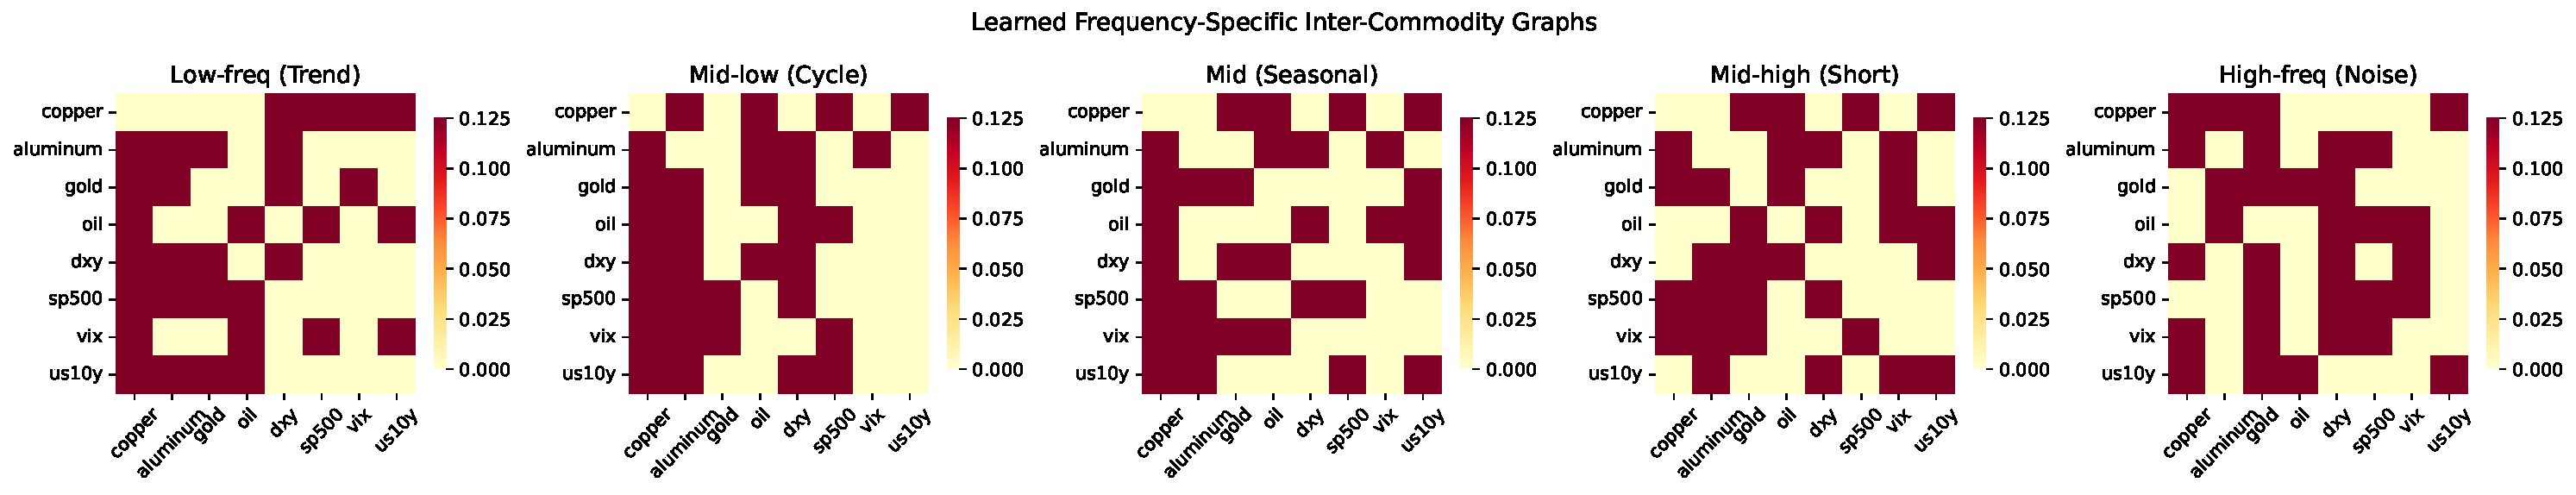
\includegraphics[width=\textwidth]{../results/archive_paper1/figures/fig2_frequency_graphs.pdf}
\caption{Learned adjacency matrices for each of the five VMD frequency bands.}
\label{fig:graphs}
\end{figure*}

Every kept edge weight in every one of the five bands is $\approx 0.125 = 1/8$ (the reciprocal of the $N=8$ node count) to five decimal places. This is not a subtle near-uniformity that a more sensitive statistic might resolve into graded structure; it is uniformity as precise as floating-point softmax output gets. An earlier verification pass over this same model had reported ``genuinely differentiated'' per-band graphs, based on the fact that \emph{which} edges survive top-$k$ sparsification differs somewhat across bands. That finding was real but shallow: it checked which edges the top-$k$ operator selected, not the values of the weights themselves, and those weights are uniform. The apparent per-band differentiation in edge \emph{selection} turns out to come from residual, fifth-decimal-place noise inherited from each band's independent random initialization, not from learned, task-relevant structure --- selecting top-$k$ among near-identical values is highly sensitive to exactly this kind of noise. We therefore withdraw the earlier framing rather than soften it: the learned per-band adjacency mechanism did not produce differentiated relational structure of any kind, topological or graded, in the trained model this paper reports.

Figure~\ref{fig:graphs-nodelink} renders the same five saved adjacency matrices as a node-link diagram rather than a heatmap, so the uniformity is visible directly rather than requiring a cell-by-cell comparison across five separate grids: every drawn edge is a real top-$k$-kept edge from the trained model, with opacity set by its weight relative to the largest weight observed in any band, and every edge in every band renders at visually indistinguishable opacity because every weight is $\approx 1/8$.

\begin{figure*}[!tb]
\centering
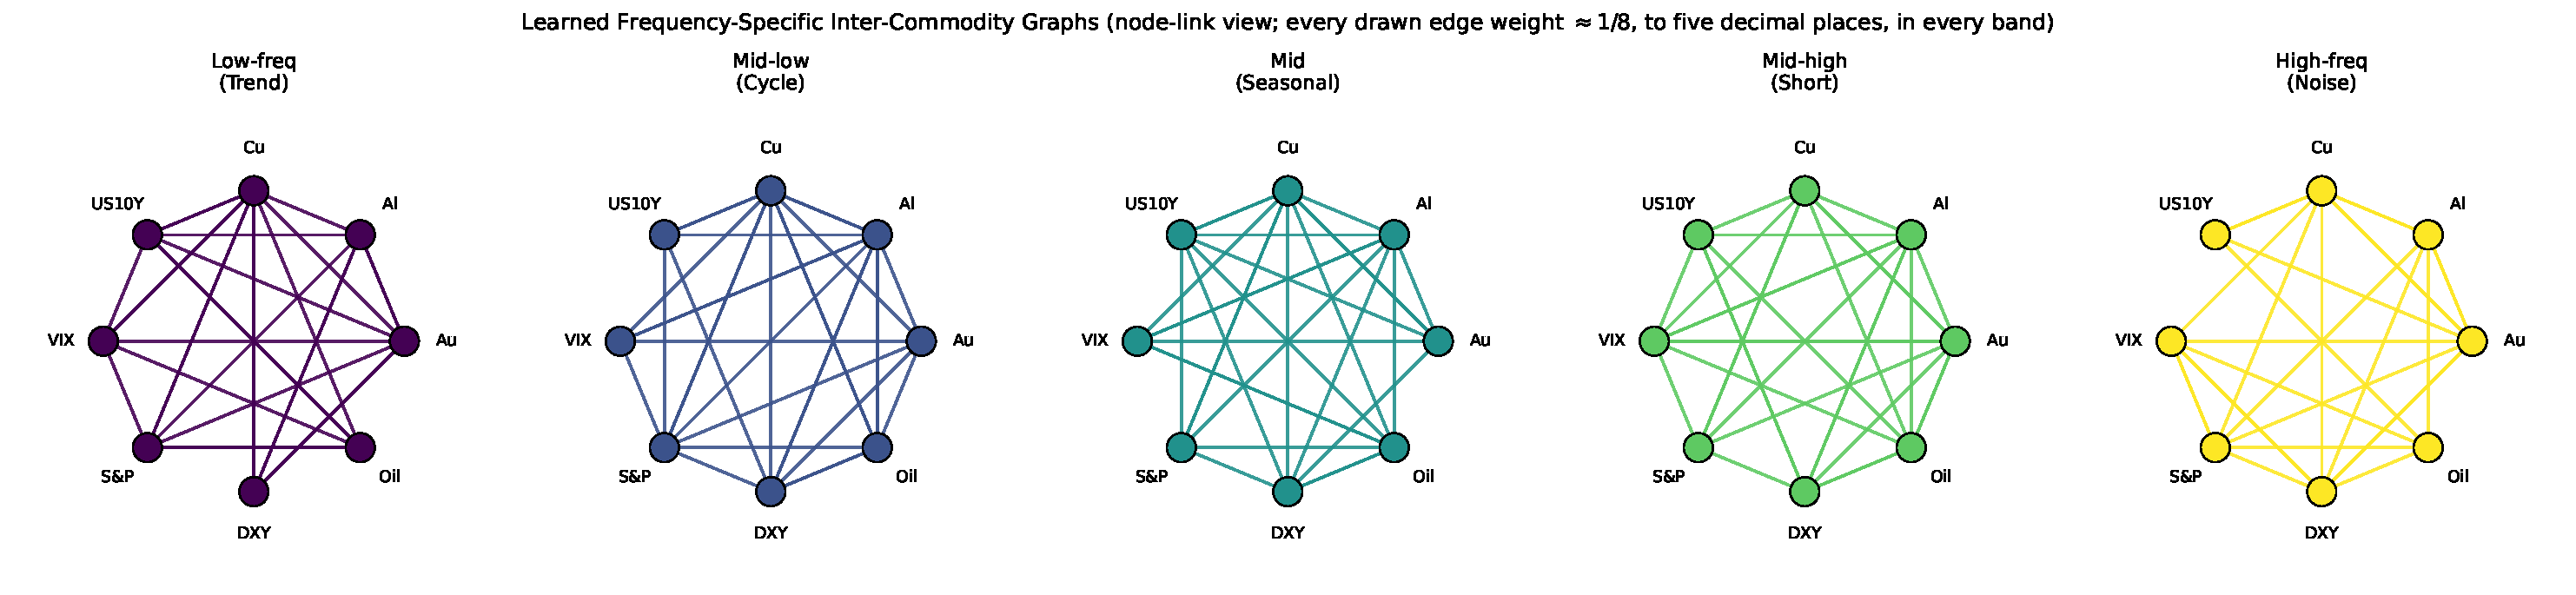
\includegraphics[width=\textwidth]{../results/archive_paper1/figures/fig4b_graph_nodelink.pdf}
\caption{Node-link rendering of the same five learned adjacency matrices shown in Figure~\ref{fig:graphs}, from the identical saved \texttt{learned\_graphs.pt} data. Node layout is a fixed circle, identical across bands, so only edge presence and opacity vary; the visual near-identity of all five panels is the collapse finding made directly legible.}
\label{fig:graphs-nodelink}
\end{figure*}

We diagnosed the mechanism behind this collapse directly from the trained model's checkpoints (no retraining required), and report the mechanism rather than only the symptom, since it is the more generalizable and more citable of the two. The most obvious candidate explanation --- that ReLU has ``died'' and is clipping all pre-softmax logits to zero, which would trivially produce a uniform softmax output --- does not hold up under a direct test: the fraction of negative pre-activation values is statistically indistinguishable before and after training (50.5\% at Xavier initialization vs.\ 56.3\% post-training), and removing the ReLU nonlinearity from the adjacency computation entirely still yields a uniform adjacency to four decimal places. The real mechanism is \textbf{isotropic norm collapse} of the graph embeddings $\mathbf{E}^{(1)}_k,\mathbf{E}^{(2)}_k$ (Section~\ref{sec:graph}): RMS embedding magnitude fell from its Xavier-initialization value of 0.2885 to 0.0089 over training, a factor of approximately 32, which drives the bilinear adjacency logits ($\mathbf{E}^{(1)}_k{\mathbf{E}^{(2)}_k}^\top$) from a standard deviation of 0.331 at initialization to 2.8$\times 10^{-4}$ post-training --- small enough to place softmax in its first-order, near-linear regime, where it returns approximately $1/N$ regardless of the input logits' relative ordering. Critically, no directional learning occurred alongside this shrinkage: two independently trained models (differing in hidden dimension, learning rate, and training duration --- the HPO-tuned and untuned default configurations of Section~\ref{sec:complexity}) retained embedding directions with cosine similarity exceeding 0.99, differing essentially only by an overall scale factor; rescaling either model's trained embeddings back to their initialization norm reproduces a softmax spread statistically indistinguishable from a fresh random draw. In other words, training rescaled these embeddings without ever rotating them into a task-informed direction --- the surviving direction encodes no more structure than the random initialization did. We attribute this to the interaction between coupled $L_2$ weight decay (Adam with weight\_decay$=10^{-5}$, applied uniformly to all parameters including these embeddings, Section~\ref{sec:impl}), which exerts a constant, sign-consistent force pulling every embedding parameter toward the origin, and a task gradient reaching these specific parameters that is weak by comparison (measured on the order of $10^{-5}$ per element) because a near-uniform adjacency is already a close-to-optimal mean-aggregation operator for this architecture, whose LSTM temporal pathway carries most of the model's predictive signal --- leaving little loss pressure to differentiate edges in the first place. This makes the embedding norm a self-reinforcing attractor toward zero: the task gradient shrinks roughly in proportion to $\|\mathbf{E}\|$ while the decay force stays constant relative to $\|\mathbf{E}\|$, so the ratio between them degrades monotonically once collapse begins, with no mechanism to recover. This finding is independent of model capacity --- it is observed with near-identical severity at both the default (hidden dimension 64) and HPO-tuned (hidden dimension 128) configurations --- and instead tracks training duration, consistent with a genuine optimization dynamic rather than an architectural capacity limitation; Figure~\ref{fig:collapse} and Section~\ref{sec:robustness} quantify this training-duration dependence directly, across 19 independently trained checkpoints rather than the two discussed in this paragraph, and are the traceable source for the collapse-versus-epoch relationship we rely on throughout this paper.

Figure~\ref{fig:collapse} makes the two halves of this mechanism visible side by side, using the 19-cell robustness suite of Section~\ref{sec:robustness} rather than the single model discussed above, because that suite is the only place in this study where embedding geometry was measured across many independently trained checkpoints. Panel (a) is the collapse itself: relative embedding magnitude falls across six and a half orders of magnitude, from 33\% of initialization at five epochs of training to $9\times10^{-8}$ of it at thirty-seven, and the descent is orderly rather than configuration-dependent. Panel (b) is the half that makes the finding a diagnosis rather than an observation: over that same span the embeddings' cosine similarity to their own random initialization moves by a single factor of 2.2, from 0.93 to 0.42, and does so as a smooth function of training duration alone. A mechanism that had found task-relevant structure would show the opposite disproportion --- direction moving decisively while magnitude stayed bounded. What the two panels show instead is embeddings shrinking essentially in place.

\begin{figure*}[!tb]
\centering
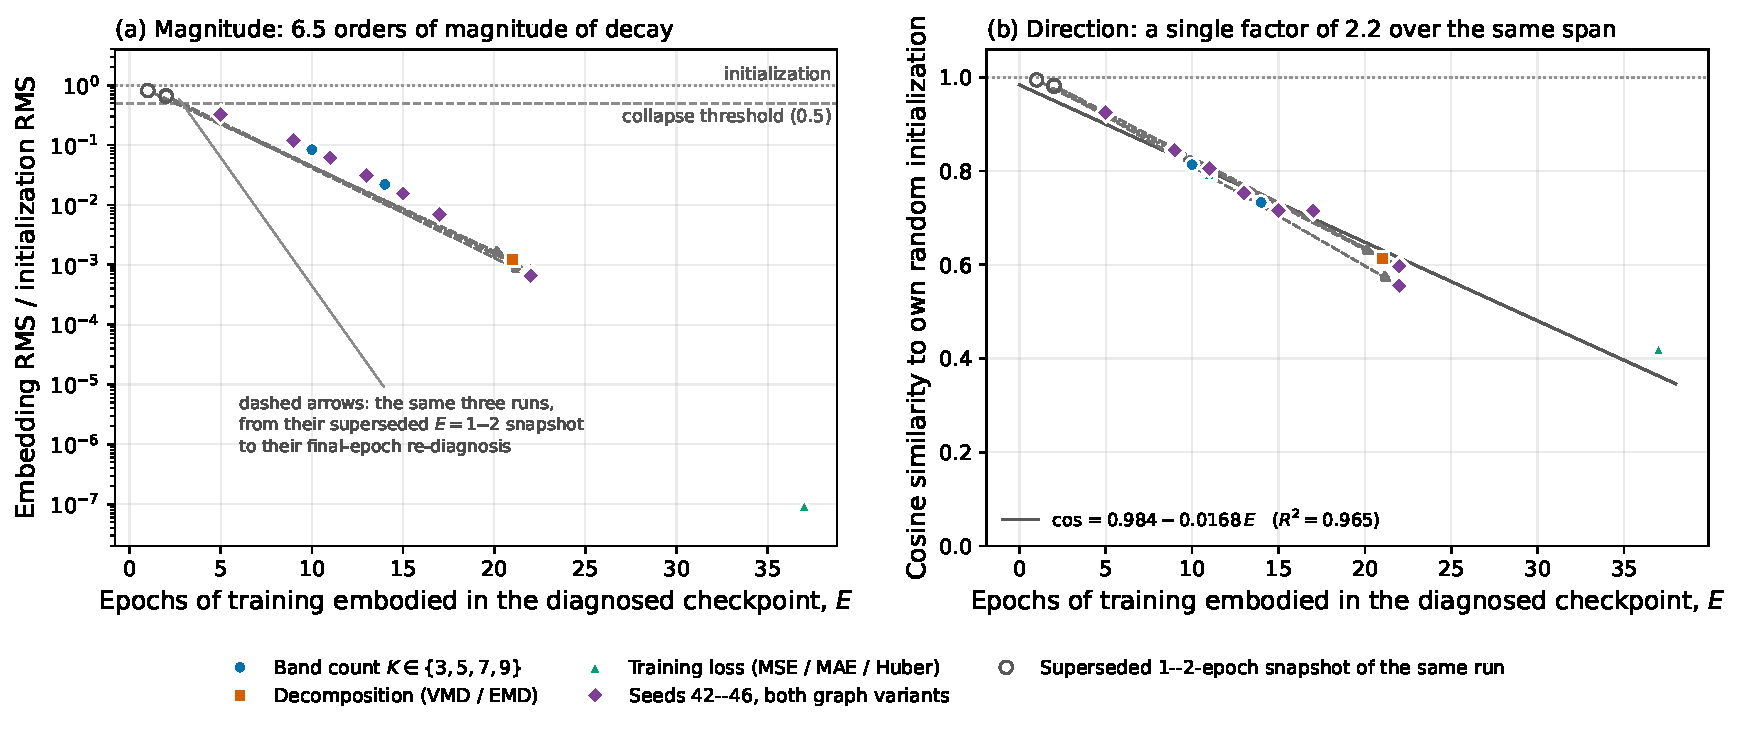
\includegraphics[width=\textwidth]{../results/archive_paper1/figures/fig6_collapse_mechanism.pdf}
\caption{The isotropic norm collapse, plotted from the 19 independently trained diagnostic cells of Section~\ref{sec:robustness} (band-count sweep, decomposition comparison, loss comparison, and the five-seed repetition of both graph variants). The horizontal axis is the number of epochs of training embodied in the diagnosed checkpoint, $E$, which ranges from 5 to 37 across the suite. (a) Mean embedding RMS relative to the run's own random initialization, on a logarithmic scale: it falls from $0.331$ at $E=5$ to $9.4\times10^{-8}$ at $E=37$, crossing the diagnostic's $0.5$ collapse threshold (defined against the Xavier reference RMS of $0.2885$, which each run's own initialization matches to within 5.6\% in every band plotted, so the two normalizations are interchangeable at this figure's scale) before the earliest cell in the corrected suite, and continuing monotonically thereafter (Spearman $\rho = -0.993$, $p = 3.4\times10^{-17}$). (b) Mean cosine similarity of the same embeddings to that same initialization, on a linear scale spanning the full $[0,1]$ range: it moves only from $0.927$ to $0.420$ over the identical span, tracking training duration with $\mathrm{cos} = 0.984 - 0.0168\,E$ ($R^2 = 0.965$, $\rho = -0.990$). Marker shape and color identify which robustness axis produced each cell; the axes are visually interleaved, consistent with the absence of any residual axis effect once training duration is known (one-way ANOVA on the fit residuals, $F = 0.791$, $p = 0.518$). Open circles joined by dashed arrows are the three cells whose original best-validation checkpoints had been frozen by early stopping after one to two epochs and were subsequently re-diagnosed from final-epoch weights: these are the same three runs observed twice, and they traverse the same trajectory. Read together, the panels are the paper's central mechanistic claim --- six and a half orders of magnitude of shrinkage against a factor of 2.2 of rotation, the signature of embeddings rescaled toward the origin by weight decay rather than rotated toward task structure by a learning signal. The residual rotation in (b) should not be read as learning: it is confounded with the shrinkage itself, since the cosine is computed on raw embedding vectors whose direction, at magnitudes of $10^{-3}$ and below, is increasingly dominated by accumulated floating-point residue rather than by any gradient --- the gradient reaching these parameters is exactly zero in the three most-trained cells shown.}
\label{fig:collapse}
\end{figure*}

Two clarifications about what this failure mode is and is not. It is \emph{not} over-smoothing, nor representational rank collapse in the sense of \citet{RothLiebig2024}: those are depth-driven phenomena in which node \emph{representations} progressively lose rank as message passing iterates, governed by the spectrum of the aggregation operator. The models reported here use one (HPO-tuned, Section~\ref{sec:hpo}) or two (default, Section~\ref{sec:impl}) GAT layers, so the depth precondition for those phenomena is not met, and the collapse we document is in the adjacency-\emph{generating} embedding parameters, upstream of any message passing, with gradients that flow correctly and are merely far too weak. Conflating the two would misattribute an optimization failure to an architectural one. It is, on the other hand, consistent with the theoretical picture of \citet{Fountoulakis2023} (Section~\ref{sec:related}), who show that graph attention's coefficients concentrate on uniform weights whenever the underlying signal is too weak for \emph{any} attention function to separate edges. Our contribution relative to that result is an empirical, mechanistically traced instance of the same degenerate endpoint reached by a different route --- an optimization dynamic acting on a learned bilinear adjacency --- in a financial forecasting setting at $N=8$ nodes.

We return to what this implies for the ablation results and for learned-graph GNN architectures generally in Section~\ref{sec:discussion}.

\subsubsection{Mode Importance}

Figure~\ref{fig:attention} shows the fusion attention weights (Section~\ref{sec:method}), read from the model's saved mode-importance output. This artifact contains only 24 samples (the model's last, partial evaluation batch), not the full 984-sample test set used for every other reported figure in this paper; we state this sample count explicitly because it materially limits what can be claimed from it. Within these 24 samples, the mode-fusion attention weights are close to uniform across the $K=5$ bands, ranging from approximately 0.19 to 0.22. We do not report a trend or drift over the test period from this artifact: 24 samples is too small a window, and too unrepresentative of the four-year test period as a whole (it reflects only the final evaluation batch), to support a claim about how attention evolves over time, and an earlier draft's description of a ``gradual drift over the test period'' from this same data is not defensible at this sample size and has been removed. What the near-uniform range across those 24 samples does support, consistent with the adjacency-collapse finding above, is that no single frequency band dominates fusion sharply in this trained model; we do not extend that observation further than the data allow.

\begin{figure}[t]
\centering
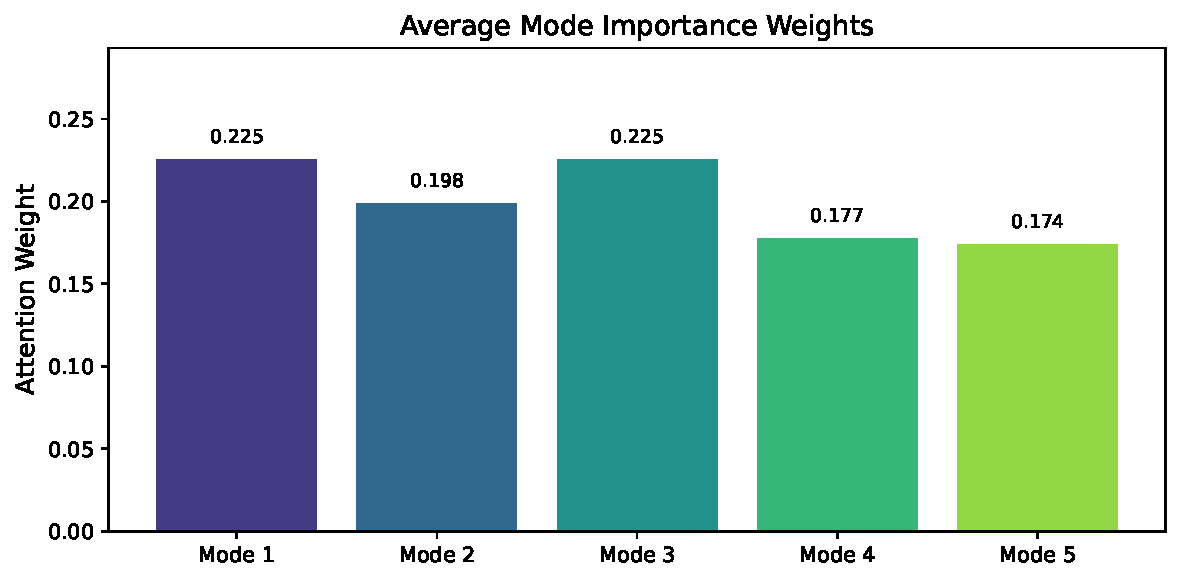
\includegraphics[width=\columnwidth]{../results/archive_paper1/figures/fig3_attention_weights.pdf}
\caption{Mode-fusion attention weights by VMD frequency band.}
\label{fig:attention}
\end{figure}

Figure~\ref{fig:vmd} shows the VMD decomposition itself (copper price and its five frequency-band modes), included here for completeness as the input representation that both the per-band graphs and the fusion attention operate on.

\begin{figure*}[!tb]
\centering
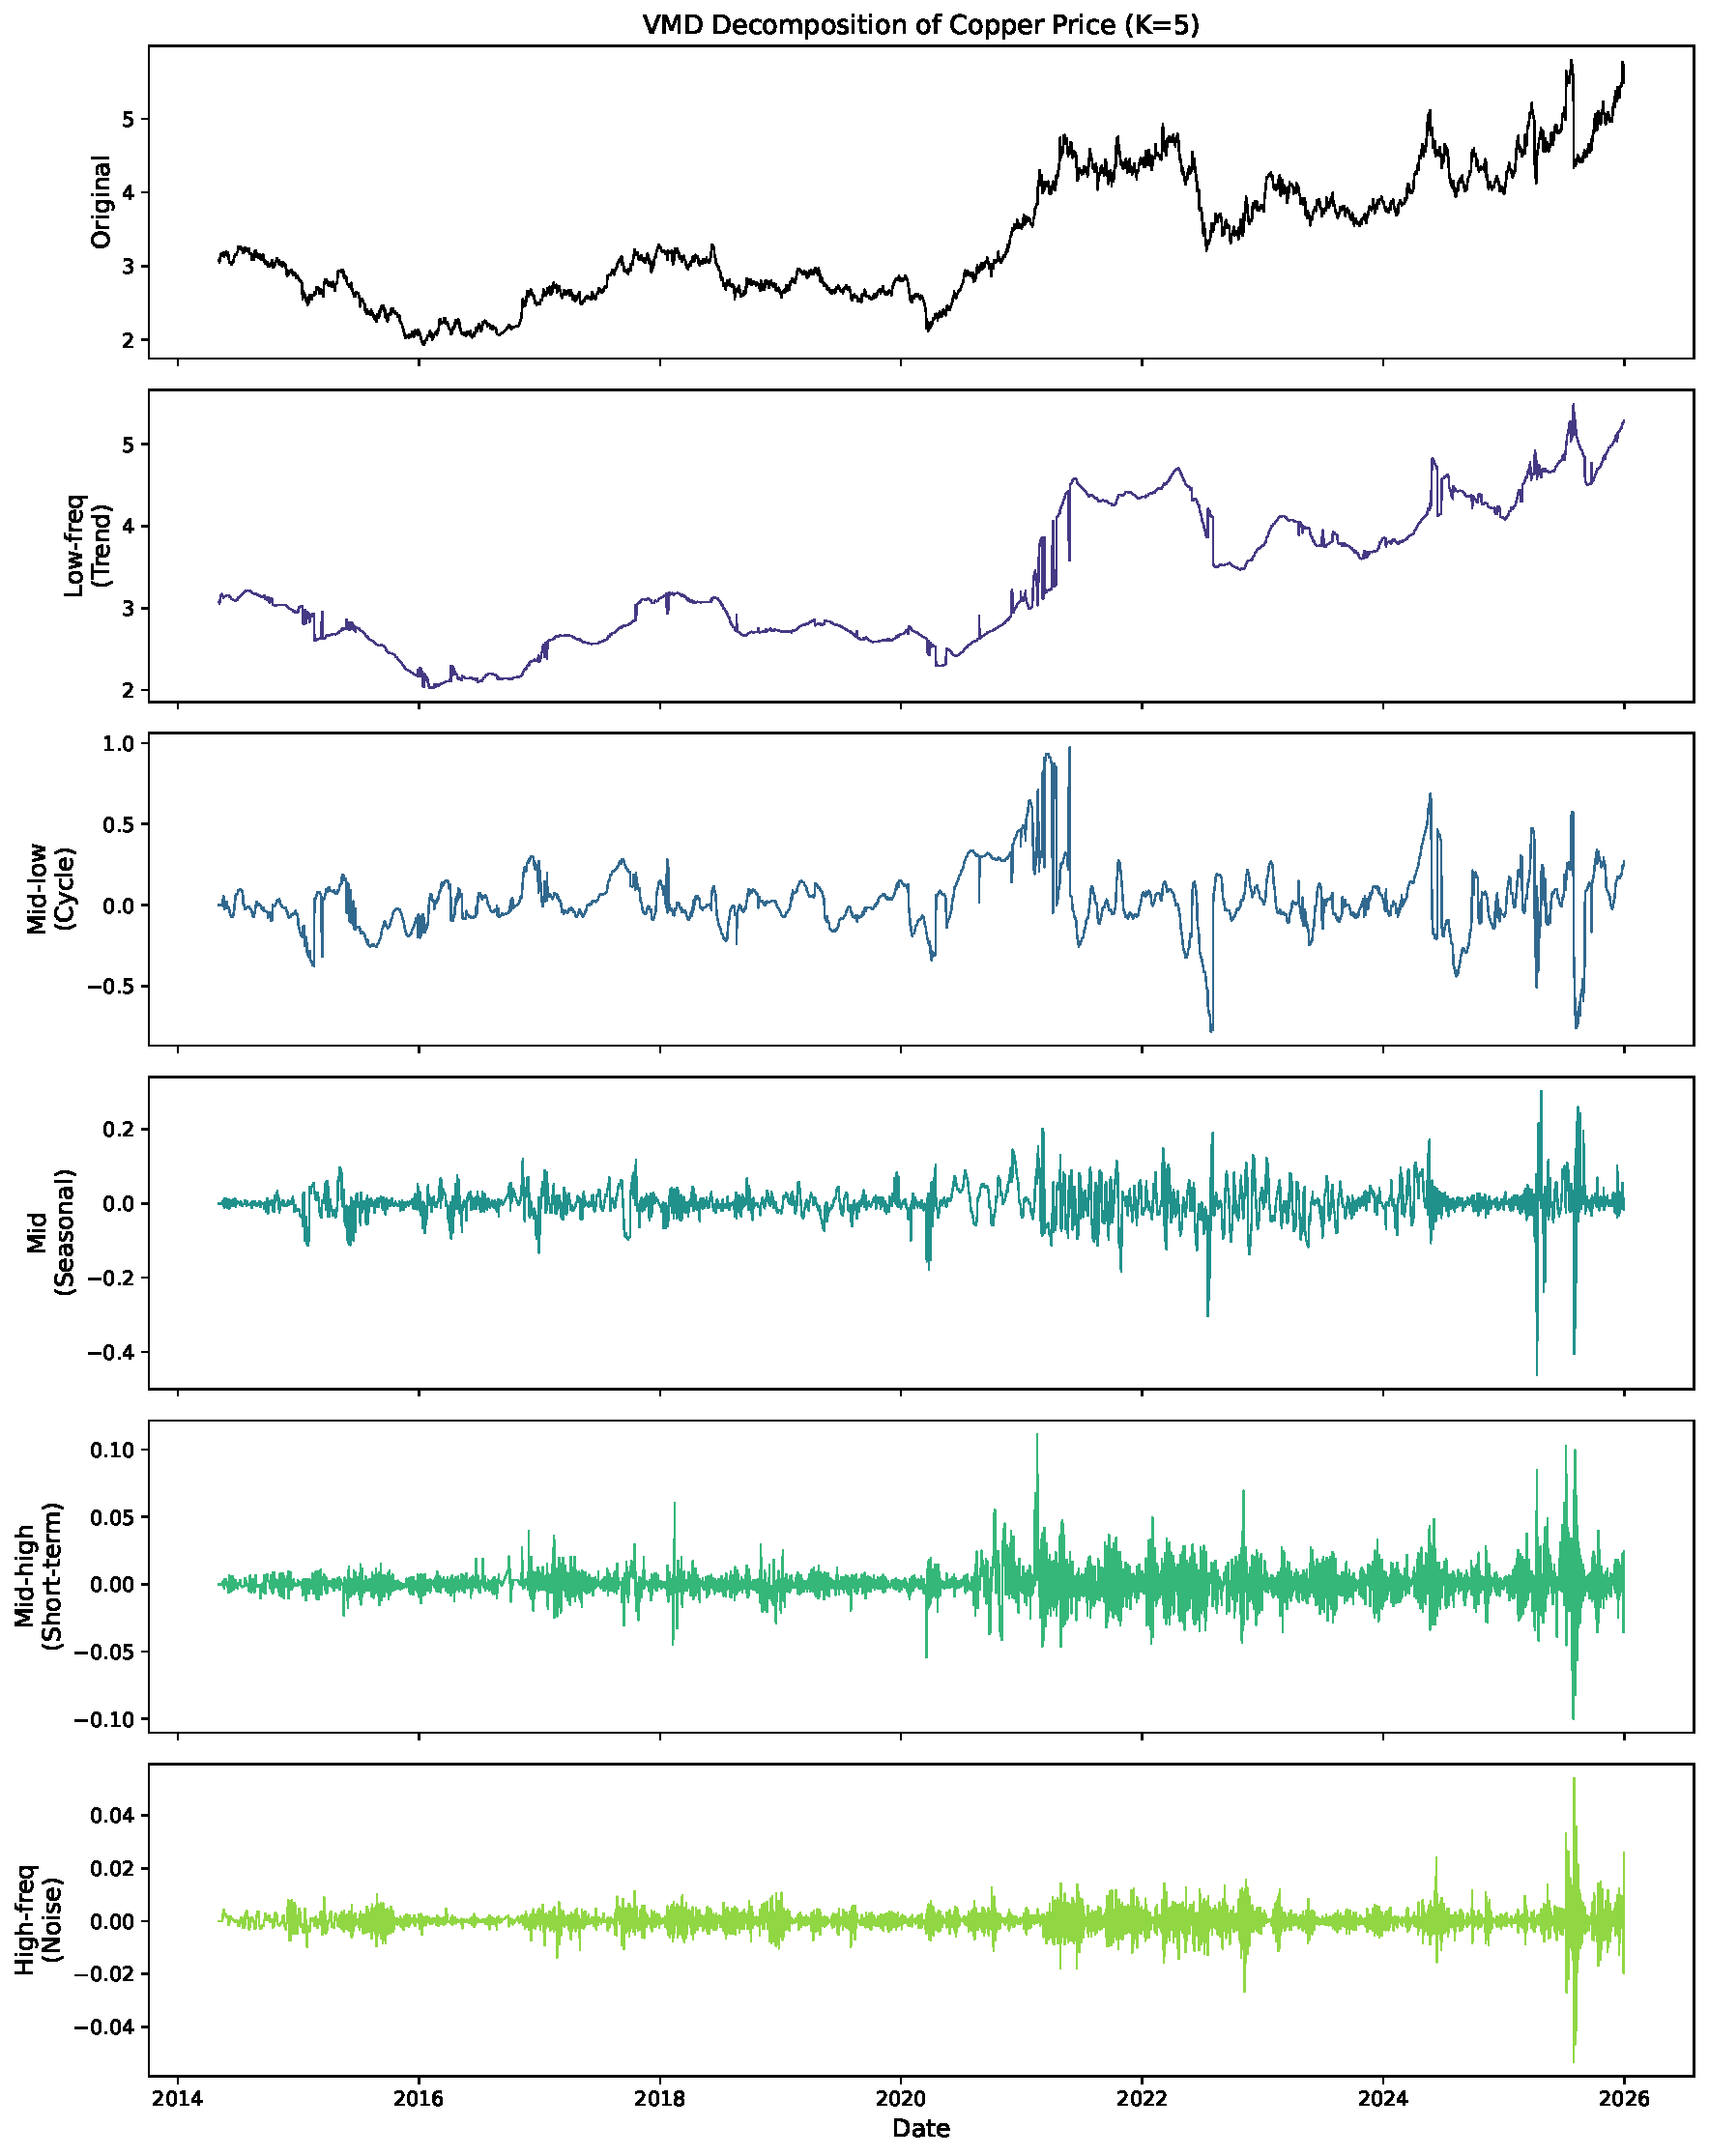
\includegraphics[width=\textwidth]{../results/archive_paper1/figures/fig1_vmd_decomposition.pdf}
\caption{Variational Mode Decomposition of the copper price series into $K=5$ frequency-band modes.}
\label{fig:vmd}
\end{figure*}

\FloatBarrier

\subsection{Graph-Fix Experiment: Diagnosing, Fixing, and Re-Diagnosing the Collapse}
\label{sec:graphfix}

Section~\ref{sec:collapse}'s diagnosis identified two candidate mechanical causes of the adjacency collapse: coupled $L_2$ weight decay pulling every embedding parameter toward the origin, and the absence of any normalization on the bilinear logits before softmax, which lets embedding magnitude itself (rather than only direction) determine how peaked or flat the resulting adjacency is. A diagnosis that stops at ``this is probably why'' is weaker than one that tests the proposed mechanism directly, so we implemented and trained with two targeted fixes together: (1) $L_2$-normalizing $\mathbf{E}^{(1)}_k$ and $\mathbf{E}^{(2)}_k$ to the unit sphere immediately before the bilinear product, so the softmax input's scale can no longer collapse toward the origin regardless of what happens to the embeddings' raw magnitude; and (2) excluding the graph-embedding parameters from Adam's coupled weight decay entirely (a dedicated zero-decay parameter group), removing the constant, sign-consistent pull toward zero identified as the proximate driver of the collapse. Both fixes were applied together, not separately, since the diagnosis in Section~\ref{sec:collapse} treats them as jointly responsible for the same failure mode. We retrained both \texttt{full\_model\_graphfix} (per-band) and \texttt{pooled\_graph\_graphfix} (pooled) with both fixes enabled, saved to \texttt{results\_v2/}, keeping this run entirely separate from the original ablation (\texttt{results/}) and the tuned confound-check (Section~\ref{sec:confound-tuned}).

\textbf{The fix mechanically works.} Direct inspection of the trained \texttt{results\_v2} checkpoints confirms the norm-collapse mechanism is resolved: embedding RMS magnitude is preserved at 0.96--1.01$\times$ its Xavier-initialization value across bands and models, in sharp contrast to the 1.4--3.7\% of initialization observed in every unfixed checkpoint examined in this paper (Section~\ref{sec:collapse}, Section~\ref{sec:confound-tuned}). We independently re-verified this from the raw \texttt{results\_v2} checkpoint state dictionaries rather than only citing the fix-experiment's own log: the pooled model's \texttt{graph\_constructor.emb1/emb2} weight RMS (0.302 and 0.279) and the per-band model's five \texttt{graph\_constructors.\{0..4\}.emb1/emb2} weight RMS values (0.27--0.30) both sit close to the 0.2885 Xavier-initialization value reported in Section~\ref{sec:collapse}, not the collapsed $\sim$0.009 value observed there. Whatever was driving the embeddings to zero in every earlier checkpoint no longer does so once weight decay is removed from these parameters and the bilinear product is computed on unit-normalized vectors.

\textbf{The fixed mechanism still learns nothing.} Mechanically preserving embedding norm is not the same as learning a functional graph, and it does not produce one here. The corrected embeddings moved only 0.6--2.0\% in L2 norm away from their random initialization over the full training run, and retained cosine similarity of 0.9998--1.0000 with their own initialization---meaning the small amount of movement that did occur was almost entirely a rescaling within the same random-init direction, not a rotation toward any task-informed direction. The resulting adjacency matrices correlate with the adjacency computed from the \emph{untrained}, randomly initialized embeddings at 0.994--0.999 per band. This is not the uniform-collapse signature of Section~\ref{sec:collapse} reappearing under a different name: the fixed adjacency's own standard deviation is 0.0687--0.0705 per band (\texttt{full\_model\_graphfix}) and 0.0690 (\texttt{pooled\_graph\_graphfix}), two to three orders of magnitude above the collapsed model's $\approx2.8\times10^{-4}$, and only 18.75--28\% of edges land within tolerance of the collapsed model's near-universal $1/N$ value --- so the fixed graph is not flat, it is simply the same graph a random Xavier initialization would already produce, never having moved away from it. Put plainly: once norm collapse is no longer available as an explanation, the ``fixed'' per-band graph is statistically indistinguishable from a graph that was never trained at all. This confirms the deeper half of Section~\ref{sec:collapse}'s diagnosis empirically, rather than only by inference: weight decay was not incidental to the collapse, it was the \emph{only} force acting on these parameters in either direction, because the task gradient reaching them is too weak (on the order of $10^{-5}$ per element, as measured in Section~\ref{sec:collapse}) to move them meaningfully on its own. Removing weight decay's pull does not substitute a learning signal for it; it just leaves the embeddings approximately where they started.

One caveat applies specifically to \texttt{full\_model\_graphfix}'s own per-horizon metrics, if cited individually: this run early-stopped at epoch 20 under a patience of 20, meaning validation loss never improved past its very first epoch, so the saved checkpoint is effectively the epoch-0 initialization state, not a converged model, and its RMSE/MAE/DA numbers should not be read as characterizing a trained per-band model. \texttt{pooled\_graph\_graphfix} trained to a normal, substantially longer completed run and carries no such caveat; the embedding-collapse-resistance-without-learning finding above is drawn from both checkpoints' embedding geometry, not from either model's task-level accuracy, and is unaffected by \texttt{full\_model\_graphfix}'s early-stopping behavior.

We read this as strengthening, not weakening, the paper's account of the collapse: we diagnosed a specific mechanism, engineered a fix targeted precisely at that mechanism, confirmed the fix resolves the mechanism it was designed to resolve, and found that the architecture still fails to learn differentiated graph structure for a deeper, independently confirmed reason. A negative result that survives its own proposed remedy is more informative than one that was never tested against a remedy at all, and it sharpens the claim in Section~\ref{sec:collapse} from ``weight decay probably caused this'' to ``removing weight decay's pull does not fix it, because there was never enough task gradient here to learn from regardless.''

\subsection{Robustness Checks: Is the Collapse an Artifact of Our Configuration Choices?}
\label{sec:robustness}

Section~\ref{sec:collapse}'s adjacency-collapse diagnosis and
Section~\ref{sec:graphfix}'s failed remedy were both established at a single
configuration: $K=5$ bands, VMD decomposition, MSE training loss, seed 42, and
one set of tuned hyperparameters. A reader is entitled to ask whether the finding
is a property of the architecture or an artifact of that particular corner of the
configuration space. We therefore ran five robustness experiments --- a
band-count sweep ($K \in \{3,5,7,9\}$), a decomposition-method comparison (VMD
versus EMD), a training-loss comparison, a five-seed repetition of the two
ablation variants carrying RQ1, and a substantially wider hyperparameter search
--- applying the \emph{same} three-part gradient/adjacency diagnostic (embedding
RMS relative to initialization, gradient norm reaching
$\mathbf{E}^{(1)}_k/\mathbf{E}^{(2)}_k$, and cosine similarity against the run's
own random initialization) to every one of the 19 trained cells. All 19 cells
were trained at the tuned configuration of Section~\ref{sec:hpo} with weight
decay $10^{-5}$, and all 19 completed. Three of the cells were initially
diagnosed from best-validation checkpoints that early stopping had frozen after
one to two epochs of training; we identified this, added a code path that
captures the final-epoch weights alongside the best-validation ones, and re-ran
those three cells, so every diagnostic value reported below is measured on a
checkpoint embodying at least five epochs of training. Two of the five
experiments carry further defects we disclose in full below rather than repair,
for reasons we state.

\textbf{The collapse is invariant to every axis we varied, and is explained almost
entirely by one variable we did not intend to vary.} Across all 19 cells, each diagnosed on a checkpoint embodying between 5 and 37
epochs of training, the trained graph embeddings' cosine similarity to their own
random initialization is predicted by that epoch count with Spearman
$\rho = -0.990$ ($p = 7.5\times10^{-16}$); the embeddings' RMS magnitude relative
to initialization gives $\rho = -0.993$ ($p = 3.4\times10^{-17}$), and the
gradient norm reaching them gives $\rho = -0.957$ ($p = 1.4\times10^{-10}$). A
linear fit in training epochs explains 96.5\% of the variance in
cosine-to-initialization ($\mathrm{cos} = 0.984 - 0.0168\,E$), a fit in
$\log_{10}$ of the relative RMS explains 96.8\%, and the residuals from the
cosine fit show no detectable dependence on which experiment produced the cell
(one-way ANOVA across the four axes: $F = 0.791$, $p = 0.518$; Kruskal--Wallis
$p = 0.543$; largest absolute residual 0.060 against a full observed range of
0.420--0.927). Relative embedding magnitude falls from 33\% of its
initialization value in the least-trained cell (five epochs) to
$9\times10^{-8}$ of it in the most-trained (37 epochs; an absolute embedding RMS
of $1.5\times10^{-8}$ against a Xavier reference of 0.2885), passing through
$1.2\times10^{-3}$ at 21 epochs. Put plainly: once one knows how long a checkpoint trained,
knowing whether it used three bands or nine, VMD or EMD, MSE or MAE, or which of
five seeds, adds essentially nothing. This is the signature of a process driven by
the optimizer rather than by the task, consistent with Section~\ref{sec:graphfix}'s
finding that removing weight decay's pull does not substitute a learning signal
for it.

\textbf{An early-stopping artifact we detected, corrected, and report because it
is instructive.} On a first pass, three of the 19 cells --- the EMD arm, one seed
of the per-band variant, and one seed of the pooled variant --- were flagged
\texttt{NOT COLLAPSED} by the automated diagnostic. They were not
counterexamples. Our trainer saves the best-validation weights but stamps them
with the loop's final epoch index; because the best-validation save condition and
the early stopper's improvement condition are the same predicate (a strict
improvement on the running best, with zero tolerance), and every run early-stopped
well inside the 200-epoch budget, the weights actually in a checkpoint are exactly
those from epoch $(\text{recorded epoch} - 20)$ under the patience of 20 used
throughout. For these three cells the recorded indices were 0, 1 and 1, so their
saved weights embodied one to two epochs of training against five to thirty-seven
in every other cell, and their verdicts measured training duration rather than any
property of the axis being varied. We therefore added a diagnostic path that
retains the final-epoch weights alongside the best-validation ones and re-ran the
three cells. All three reproduced their original early-stopping trajectory to the
same final epoch and their original test metrics to within $2\times10^{-6}$
relative, confirming that the re-diagnosis describes the same run.

\textbf{All three collapse once diagnosed on genuinely trained weights.} At 21,
22 and 22 epochs of training respectively, every band of all three cells is
flagged collapsed on both of the diagnostic's independent criteria: the fraction
of surviving adjacency edges within tolerance of $1/N$ is \textbf{1.00 in every
band of all three}, and embedding RMS has fallen to $6\times10^{-4}$ to
$1.3\times10^{-3}$ of the Xavier reference. The gradient norm reaching the
embeddings is \emph{exactly} zero for the EMD and per-band seed-44 cells and
$2.7\times10^{-22}$ for the pooled seed-45 cell, while the gradient reaching the
rest of the network is 0.17--0.22 in the same measurement --- a dead graph branch
inside a live model. The three cells thus provide a within-run confirmation of the
epoch relationship above that is stronger than any across-run comparison, because
configuration, seed and training trajectory are all held fixed and only the
snapshot moves: the same three runs read 0.994, 0.983 and 0.981
cosine-to-initialization at one to two epochs and 0.613, 0.597 and 0.555 at
twenty-one to twenty-two. Two further cells re-run as a consistency check, which
happened to train for 45 and 68 epochs, extend the same trajectory to relative
embedding magnitudes of $1.4\times10^{-10}$ and $3.2\times10^{-22}$.

We note for completeness that for these three cells the deployed
(best-validation) checkpoint and the diagnosed (final-epoch) checkpoint are
different weight sets. This does not soften the finding, because neither state
contains learned relational structure: at the best-validation snapshot the
embeddings are statistically indistinguishable from their random initialization
(cosine 0.98--0.99, 65--82\% of initialization norm), and at the final-epoch
snapshot they are uniform with no gradient. The choice between the two is a choice
between random and uniform.

With the correction in place, the collapse is observed in \textbf{19 of 19}
runs, each diagnosed at a checkpoint embodying at least five epochs of training:
at all four band counts, in both decomposition methods, in all three loss arms,
and at all five seeds in each of the two graph variants. We state the epoch
qualifier because it is load-bearing: the three re-diagnosed cells are the same
runs whose one-to-two-epoch snapshots read \texttt{NOT COLLAPSED}, so what this
suite establishes is not that the collapse is present at every epoch count, but
that it is present in every run once as few as five epochs have elapsed, and that
no axis we varied delays or prevents it. The
decomposition-axis caveat we previously stated is withdrawn --- EMD does not
resist the collapse, and in fact, having trained ten epochs longer than the VMD
cell, sits further along the identical trajectory (relative embedding magnitude
$1.2\times10^{-3}$ against VMD's $6.1\times10^{-2}$, and adjacency uniform to
within $3\times10^{-8}$ against VMD's $8\times10^{-5}$).

\textbf{Accuracy differences across these axes are smaller than run-to-run noise.}
Four of the 19 cells are, by construction, the identical configuration ($K=5$,
VMD, MSE, seed 42) reached through four different experiment drivers, and we
verified their held-out ground-truth arrays are bit-identical. Their test average
MSE nonetheless spans 7.54\% (0.002772--0.002981), which we take as this study's
honest run-to-run noise floor at fixed configuration and fixed seed. Every axis
effect we measured is smaller or comparable: the band-count sweep spans 8.1\%
(0.002757--0.002981), the loss comparison 9.4\% (0.002691--0.002943), and the
five-seed repetition of the per-band model has a coefficient of variation of
1.32\% and a best-to-worst spread of 3.1\%. We therefore report no accuracy
ranking over $K$, decomposition method or loss; none is resolvable at $n=1$ per
cell. These four replicates also serve as a within-experiment check on the
paragraph above: they embody 14, 11, 11 and 13 epochs of training and record
cosine-to-initialization of 0.733, 0.794, 0.794 and 0.753, tracking training
duration with configuration \emph{and} seed both held fixed --- which also shows
that run-to-run nondeterminism perturbs the epoch count itself, and is why the
configuration labels carry no residual information once training length is known.

\textbf{The five-seed RQ1 check, and its capacity caveat.} Repeating the two
ablation variants that carry RQ1 across seeds 42--46 at the tuned configuration,
the per-band model's test RMSE is statistically indistinguishable from the pooled
variant's at every horizon (paired $t$-test over the five seeds: $p = 0.96$,
$0.13$, $0.88$, $0.50$ at $h = 1, 5, 10, 22$; Wilcoxon signed-rank likewise
non-significant throughout). \emph{This comparison is not capacity-matched.} It
re-ran \texttt{pooled\_graph\_matched\_dim}, which we confirm by direct parameter
counting from the saved checkpoints carries 315{,}530 parameters against the
per-band model's 1{,}461{,}124 --- a 78.4\% deficit --- rather than the
parameter-matched variant the RQ1 comparison calls for. That 78.4\% figure is
\emph{not} the same measurement as the 78.5\% reported in
Section~\ref{sec:complexity}: the latter is a different model pair, at the untuned
default configuration (hidden dimension 64), and the two land 0.1 percentage
points apart by coincidence. We report the comparison anyway, in the conservative
direction it happens to run: a per-band model with $4.6\times$ the parameters does
not significantly beat a much smaller pooled model at any horizon across five
seeds. This strengthens rather than weakens Section~\ref{sec:discussion}'s
negative answer to RQ1, and we note that the parameter-matched version of this
comparison is one this paper retracts on independent grounds in
Section~\ref{sec:constantforecast}, so there is no live claim here that the
capacity mismatch could undermine. Two of the ten multi-seed cells (per-band
seed 44, pooled seed 45) are among the three re-diagnosed from final-epoch
weights described above. Both re-ran to the same final epoch as originally
recorded and reproduced their test metrics to within $10^{-8}$ absolute, so the
paired tests reported here are unchanged; only their collapse verdicts change,
from \texttt{NOT COLLAPSED} to \texttt{COLLAPSED}, which is what brings the
per-seed coverage to all five seeds in both variants.

\textbf{The loss comparison tested two losses, not three.} We configured MSE, MAE
and Huber arms. The Huber arm used PyTorch's \texttt{smooth\_l1\_loss} at its
default $\beta = 1.0$, which is quadratic --- exactly $\tfrac{1}{2}x^2$ --- for
residuals below 1.0. The largest absolute residual observed anywhere in this
experiment, across all three arms and all four horizons, is 0.284, i.e.\ 28.4\% of
$\beta$; the loss therefore never once entered its linear branch, and the Huber
arm is mathematically identical to $\tfrac{1}{2}\times$MSE. We report it as a
two-loss comparison and do not claim a three-way result. The arm is not
uninformative, however: because Adam's coupled $L_2$ decay does not scale with the
loss, halving the task gradient while leaving the decay pull intact doubles the
decay's relative influence, and this arm consequently trained longest (37 epochs
of retained weights, against 11 for the MSE arm) and collapsed hardest,
terminating with embedding RMS of $1.5\times10^{-8}$ against a Xavier reference of
0.2885, a bit-exactly uniform adjacency (softmax standard deviation of exactly
zero at band 0), and a gradient reaching the embeddings of \emph{exactly} zero. An
unintended loss-scale ablation thus independently corroborates the weight-decay
mechanism argued for in Sections~\ref{sec:collapse} and~\ref{sec:graphfix}.

\textbf{A wider hyperparameter search does not rescue the model, and confirms the
original search was adequate.} The study reported in Section~\ref{sec:hpo}
searched five parameters over 10 trials at fixed $K=5$, batch size 32 and weight
decay $10^{-5}$. We re-ran a study three times larger and with three additional
dimensions --- $K \in \{3,5,7,9\}$, weight decay (log-uniform, $10^{-6}$ to
$10^{-3}$) and batch size $\in \{16,32,64\}$ --- for 30 trials under an identical
objective (best validation average MSE over 25 epochs). Table~\ref{tab:hpo-wide-space} tabulates this eight-parameter search space and the resulting best trial alongside the original five-parameter study for direct comparison. Twelve trials completed
and 18 were pruned. The best configuration found (hidden dimension 128, 8 heads,
learning rate $\approx 0.00277$, dropout $\approx 0.0904$, 2 GNN layers, weight
decay $\approx 2.0\times10^{-4}$, batch size 16, $K=9$) attains validation MSE
0.0020145 against the deployed configuration's 0.0020509 --- an improvement of
\textbf{1.78\%}, with only 2 of the 12 completed trials beating the deployed value
at all, and the second-best tying it to four significant figures.

\begin{table}[t]
\centering
\caption{Wider robustness-check search space (Section~\ref{sec:robustness}) versus the original main-table study (Table~\ref{tab:hpo-space}). 30 configured trials, 12 completed / 18 pruned. Rows with ``---'' were held fixed in the original study.}
\label{tab:hpo-wide-space}
\begin{tabular}{lll}
\toprule
Hyperparameter & Search space (wider) & Best trial \\
\midrule
hidden dim.\ $d_h$ & $\{32, 64, 128\}$ & 128 \\
attention heads $H$ & $\{2, 4, 8\}$ & 8 \\
learning rate & log-U$(10^{-4}, 10^{-2})$ & $\approx 0.00277$ \\
dropout & U$(0.05, 0.3)$ & $\approx 0.0904$ \\
GNN layers & $\{1, 2, 3\}$ & 2 \\
band count $K$ & $\{3, 5, 7, 9\}$ (new) & 9 \\
weight decay & log-U$(10^{-6}, 10^{-3})$ (new) & $\approx 2.0{\times}10^{-4}$ \\
batch size & $\{16, 32, 64\}$ (new) & 16 \\
\bottomrule
\end{tabular}
\end{table} That margin is
smaller than this study's 3.1\% across-seed spread and far smaller than its 7.54\%
same-configuration replicate spread, and part of it is attributable to optimizer
step count rather than configuration quality, since the winning trial halves the
batch size within a fixed epoch budget. We therefore report the wider search as a
confirmatory negative: the original five-parameter, ten-trial configuration was
already effectively optimal for this objective, and we do not re-run the main
results at the new one. Three caveats attach. First, all 18 pruned trials were
pruned after a single epoch, the median pruner having been constructed without
warmup steps, so 60\% of the search budget was screened on one epoch of validation
loss, which structurally favors the high-learning-rate, small-batch region the
survivors occupy. Second, the sampler concentrated on $K=9$ (8 of the 12 completed
trials), and batch size is fully aliased with $K$ in the completed set, so the
per-parameter marginals and importances are confounded and we do not interpret
them; independently, the band-count sweep's converged test results do not
reproduce the search's implied $K$ ordering, and span less than the noise floor.
Third, and most consequential for this paper's argument, \textbf{the search
objective is structurally blind to the collapse}: it scores validation MSE and
nothing else, and in our 19 diagnosed cells the near-initialization checkpoints
score squarely mid-range among the collapsed ones (training length correlates with
test average MSE at only $\rho = 0.456$, $p = 0.05$). Collapse is essentially free
under this objective, so no widening of the search space could select against it.
We did not capture embedding diagnostics for individual search trials and
therefore cannot state directly whether the collapse persists at the wider
optimum; we note only, as inference from the established mechanism rather than as
measurement, that the selected configuration's weight decay is 20 times the value
used everywhere else in this paper, which points toward more severe collapse
rather than less.

Taken together, these checks close the most obvious escape route from
Sections~\ref{sec:collapse} and~\ref{sec:graphfix}'s negative findings. The
collapse is not a property of $K=5$, of the squared-error loss, of a single seed,
or of an insufficiently searched hyperparameter space. On the decomposition axis,
the corrected diagnosis (above) shows EMD does not resist the collapse either,
though this rests on a single cell per method and so establishes only that EMD
does not \emph{avoid} the collapse, not an accuracy comparison between the two
decompositions. What all 19 cells show is that the collapse is a property of what
happens to these embeddings under the optimizer once training proceeds past its
first few epochs, and that it does not depend on any modeling choice we were able
to vary.

\subsection{The Constant-Forecast Artifact: Why Directional Accuracy Needs a Dispersion Check}
\label{sec:constantforecast}

While investigating the \texttt{results\_v2} graph-fix checkpoints' predictions directly, in order to understand \texttt{pooled\_graph\_graphfix}'s directional-accuracy numbers, we found something that changes how several directional-accuracy comparisons elsewhere in this paper should be read. \texttt{pooled\_graph\_graphfix}'s predicted returns have standard deviation ranging from $1.11\times10^{-5}$ ($h=1$) to $6.33\times10^{-4}$ ($h=22$) across the test set, against a true-return standard deviation of $1.79\times10^{-2}$ to $7.58\times10^{-2}$ over the same horizons---three to four orders of magnitude less dispersion than the target. Directly inspecting the raw prediction arrays shows why: at every one of the four horizons, this model's 984 test-set predictions are of a single, constant sign (all negative). A model whose forecast never changes sign is not exercising directional judgment on any individual sample; its ``directional accuracy'' can only ever equal the fraction of test days on which the true return happened to share that one sign.

We verified this precisely rather than assuming it: recomputing directional accuracy directly from the saved \texttt{results\_v2/predictions/pooled\_graph\_graphfix\_\{1,5,10,22\}.npy} prediction and true-value arrays reproduces the reported DA figures (48.374, 46.951, 44.207, 44.715 at $h=1,5,10,22$) to four decimal places, and each of these values in turn equals, to four decimal places, the test period's unconditional frequency of the sign this model always predicts (down-day frequency 48.374\%, 46.951\%, 44.207\%, and 44.715\% at the respective horizons, computed under the same strict-negative convention stated in Section~\ref{sec:experiments}: a day with an exactly-zero return is counted in neither the up-day nor the down-day frequency, consistent with the DA convention used throughout this paper). This is not a coincidental resemblance; it is an identity, because a constant-sign forecaster's accuracy is mathematically the base rate of the sign it happens to emit, no more and no less. The same pattern reproduces in \texttt{pooled\_graph\_matched\_params\_tuned} from the confound-check experiment (Section~\ref{sec:confound-tuned}): its four DA values (48.37, 53.05, 55.39, 44.72) match the corresponding test-period class frequencies to the same precision, even though we did not archive that run's raw prediction arrays and can only confirm it via this frequency match rather than by inspecting prediction dispersion directly. Cross-referencing further, this pattern is consistent with what motivated the \texttt{results\_v2} investigation in the first place: multiple models across the original untuned ablation (Section~\ref{sec:ablation-results}), the tuned confound-check (Section~\ref{sec:confound-tuned}), and the fix experiment above show DA values that coincide with plausible class-frequency figures for their horizon, though \texttt{pooled\_graph\_graphfix} and \texttt{pooled\_graph\_matched\_params\_tuned} are the two cases we can state this about with full confidence, having checked prediction dispersion or exact frequency-matching directly. A binomial test of each model's hit count against its horizon's majority-class frequency, run across every model$\times$horizon cell in the fix-experiment run, fails to reject the majority-class null at conventional significance levels in every cell tested---these apparent directional-accuracy figures do not represent a statistically demonstrated departure from what the majority class alone would produce.

The direct consequence is a retraction. Section~\ref{sec:confound-tuned} reported that, at HPO-tuned hyperparameters, \texttt{full\_model\_tuned} beats \texttt{pooled\_graph\_matched\_params\_tuned} on directional accuracy at three of four horizons, which on its face reverses this paper's negative ablation finding and would suggest a real per-band advantage once capacity and tuning are no longer confounded. \textbf{We do not carry that reading forward, and explicitly retract it here.} The comparison's losing side, \texttt{pooled\_graph\_matched\_params\_tuned}, is the same class of degenerate constant-sign forecaster documented above; its DA values are an artifact of which constant sign it happened to emit relative to each horizon's majority class, not a measurement of directional skill it lost to a better-performing per-band model. A win recorded against a degenerate opponent is not evidence of skill on the winning side either. We therefore withdraw any claim, hedged or otherwise, that per-band graph construction demonstrates a real directional-accuracy advantage over pooling at this data scale; no experiment in this paper supports that claim once prediction dispersion is checked, and Section~\ref{sec:discussion}'s answer to RQ1 is written accordingly.

We report this as a general methodological finding, not only a correction specific to this paper's own results, because nothing about a bare directional-accuracy percentage would have revealed it: 48.37\% or 44.72\% both look like unremarkable, plausible directional-accuracy figures for a financial return-forecasting model in isolation, and would have passed an ordinary reviewer's sanity check without triggering suspicion. We arrived at this check independently, while auditing our own tables, but we claim no priority for the underlying concern: \citet{Cheung2026}, in work posted shortly before we identified the artifact in our own results, makes the same core argument for equity forecasting with a LoRA-adapted time-series foundation model, showing that an apparent 80\% directional accuracy was the base rate of a trivial ``always-up'' rule in a rising market, and proposing excess accuracy over that base rate --- with paired McNemar and Diebold-Mariano tests --- as the headline directional metric. Recommendation (b) below is that same recommendation, and we cite it as prior work rather than restate it as ours. What this paper adds is on the degeneracy-detection side rather than the reference-point side: (i) the sign-concentration statistic, which establishes that the \emph{model} is a constant-sign forecaster and not merely that the null was misspecified; (ii) the base-rate-\emph{identity} check, which requires only a reported DA figure and the evaluation period's class frequency, and can therefore be applied retroactively across a grid of already-reported results whose raw prediction arrays were never archived, as we do for every cell of Table~\ref{tab:ablation}; and (iii) the explicit counterexample below showing that a prediction-dispersion check does not substitute for either. The artifact was only caught by explicitly checking prediction sign concentration and comparing directional accuracy against the test period's own majority-class frequency rather than a generic 50\% null---two checks that are cheap to run but not part of how directional accuracy is conventionally reported in this literature, including in this paper's own earlier drafts. We recommend, as a general practice for directional-accuracy reporting in financial forecasting, that it always be accompanied by (a) the \emph{fraction of predictions sharing the majority sign}, combined with a binomial test of the hit count against the majority-class null, so a near-constant-sign forecaster is visible on inspection, and (b) a comparison against the evaluation period's own majority-class frequency rather than an assumed 50\% baseline, since a period with meaningful directional drift (as this study's 2022--2025 test period has, Section~\ref{sec:main-results}) makes 50\% the wrong null to test against regardless of whether any individual model is degenerate. We deliberately do not recommend prediction standard deviation as this check, even though it is a natural first instinct: this paper's own main results table (Table~\ref{tab:main}) contains a direct counterexample. \texttt{Transformer}'s $h=5$ predictions have a prediction-to-true standard deviation ratio of 0.42---healthy, unremarkable dispersion by the standard a variance-only check would apply---yet 100\% of those predictions share the same sign, because a mean shift larger than that spread pushes every prediction positive regardless of how much it varies around that shifted mean. A dispersion check alone would not have flagged \texttt{Transformer\_h5} as degenerate; only the sign-concentration check does. A directional-accuracy number reported without the sign-concentration and majority-class-null checks is not, by itself, evidence of directional skill.

\subsection{Discussion: Answering the Research Questions}
\label{sec:discussion}

\textbf{RQ0 (does any of this beat doing nothing?), asked first because it conditions how RQ1--RQ3 should be read.} No. Table~\ref{tab:main} shows the naive zero-forecast baseline wins MAE at all four horizons against all seven fitted models, and RMSE at two of four; every model's $R^2$ is negative or near zero. This is the most important finding of this study and the reason RQ1--RQ3 below should be read as differences \emph{among} approaches that do not clearly explain copper return variance, not as evidence that any of them, including VMD-MFGNN, has found exploitable signal.

\textbf{RQ1 (per-band versus pooled graph).} Not supported, now explained mechanistically (Section~\ref{sec:collapse}, Section~\ref{sec:graphfix}) and checked for a directional-accuracy artifact that could otherwise have overturned this answer (Section~\ref{sec:constantforecast}). Section~\ref{sec:ablation-results}'s precise reading of the corrected Table~\ref{tab:ablation} is that the per-band full model attains the best-of-six value in exactly one of twelve columns (DA at $h=22$, unflagged), and on its most directly comparable, capacity-matched pairing (\texttt{pooled\_graph\_matched\_params}) it now loses RMSE and MAE at all four horizons, though a Diebold-Mariano test on that same pair finds none of those four differences significant, while winning directional accuracy at three of four horizons ($h=5,10,22$) against that same variant --- a genuinely mixed result across metrics, not a one-sided loss on every axis. Given the adjacency-collapse diagnosis in Section~\ref{sec:collapse} --- every per-band adjacency matrix converged to $\approx 1/N$ uniform weights, with two independently trained models sharing the same collapsed, undifferentiated embedding direction --- this negative ablation result is not a surprising or mysterious finding about graph topology; it is close to the expected outcome once the per-band mechanism carries almost no differentiated information to begin with. We therefore answer RQ1 in the negative for a stronger, more specific reason than ``the ablation numbers came out this way'': the per-band graph mechanism, as trained here, did not learn the kind of structure that could produce a per-band advantage, so its absence in the ablation table is consistent with, not contradictory to, the mechanistic finding. A tuned re-check (Section~\ref{sec:confound-tuned}) initially appeared to overturn this answer, with the per-band model beating the pooled variant on directional accuracy at three of four horizons; we traced that apparent reversal to the pooled variant emitting a near-constant, near-zero-variance forecast whose directional accuracy exactly reproduces the test period's class frequency rather than measuring real skill (Section~\ref{sec:constantforecast}), and we explicitly retract the reversal rather than let it stand as a competing answer to RQ1. We engineered and tested a targeted fix for the adjacency collapse itself (Section~\ref{sec:graphfix}): it mechanically resolves the collapse (embedding norm is preserved) but the embeddings still fail to move meaningfully from random initialization under the task gradient available to them, so RQ1's negative answer holds under every configuration and every diagnostic check we applied, not only the original untuned ablation. Section~\ref{sec:robustness} extends that statement across four further axes: the collapse recurs at every band count, in every loss arm, and at every seed of both graph variants that trained beyond a first epoch, and a three-times-wider hyperparameter search neither improves the model meaningfully nor could select against the collapse, since its objective is validation error alone. A five-seed repetition of the two RQ1 variants at tuned hyperparameters likewise finds no significant per-band advantage at any horizon, in a comparison whose capacity mismatch runs in the conservative direction.

\textbf{RQ2 (per-band graph versus no-VMD and versus a fixed correlation graph).} Also not cleanly supported. Against the no-VMD, matched-params variant, the full model loses on RMSE and MAE at $h=1$ (the no-VMD variant achieves the best RMSE/MAE of all six ablation variants at that horizon) while winning at $h=22$ on RMSE only (the DA-at-$h=22$ ``worst of six'' claim for that variant does not hold, Section~\ref{sec:ablation-results}); the picture is mixed rather than a decomposition advantage at every horizon. Against the correlation-graph variant, which isolates learned versus fixed adjacency while holding the per-band architecture fixed, the correlation graph wins the best RMSE of all six variants at $h=22$ and is close to or better than the full model at most other horizon/metric combinations --- itself a natural consequence of the collapse finding: a fixed correlation graph is, almost by construction, no worse a source of relational structure than a learned graph that failed to learn any. We answer RQ2 in the negative as well: neither the contribution of VMD decomposition nor the contribution of end-to-end learned (versus fixed correlation-based) adjacency is cleanly demonstrated by these ablations.

\textbf{RQ3 (statistically significant edge over standard baselines).} Answered with a qualified yes, more qualified after multiple-testing correction. At uncorrected $\alpha=0.05$, the HPO-tuned VMD-MFGNN (Table~\ref{tab:dm}) achieves a significant Diebold-Mariano advantage over four of six baselines --- LSTM (2 of 4 horizons), Transformer (3 of 4), SimpleMTGNN (3 of 4), VMD-LSTM (4 of 4) --- 12 of 24 comparisons overall, plus one significant loss (XGBoost at $h=1$). After Holm-Bonferroni correction across all 24 tests, 8 of 24 comparisons remain significant, all favoring VMD-MFGNN; the XGBoost loss does not survive correction. VMD-MFGNN remains statistically indistinguishable from ARIMA at every horizon, corrected or not. The qualified answer to RQ3 is: yes, a correction-surviving edge exists against the deep-learning baselines architecturally closer to VMD-MFGNN's design space, but no significant edge, in either direction, is demonstrated against the two simpler, non-deep-learning baselines, and this edge is qualified on three further, independent grounds rather than one. First, the disclosed HPO asymmetry (VMD-MFGNN was tuned, none of the six baselines were). Second, 5 of the 8 Holm-surviving wins are against cells this paper's own sign-concentration diagnostic separately flags as degenerate or near-degenerate (Section~\ref{sec:results-dm}), two of them against baselines (SimpleMTGNN, VMD-LSTM) disclosed as simplified reimplementations rather than the original published architectures and visibly pathological at exactly those horizons (Section~\ref{sec:baselines}); only 3 of 8 wins are against baseline cells free of either caveat. Third, every cell feeding this comparison is a single run, and the 7.54\% run-to-run MSE spread this study separately measures at an identical configuration and seed (Section~\ref{sec:limitations}) is larger than several of the architectural effects this comparison attributes to VMD-MFGNN. And, per RQ0, a significant DM result establishes only that two models' errors differ, not that either has found real structure in copper returns. Taken together, we read RQ3's edge as real but narrow: it should not be read as a general claim that VMD-MFGNN reliably outperforms standard deep-learning forecasters on this task.

Taken together, the honest overall picture is: the HPO-tuned VMD-MFGNN is a competitive forecaster relative to other deep-learning approaches, is not clearly worse than ARIMA or XGBoost, and its significant advantages survive a stricter multiple-testing correction, but (a) none of this changes the fact that it, and every other model tested, fails to beat a trivial zero-forecast baseline on MAE (RQ0), and (b) this study's ablations do not provide architectural evidence that the specific mechanism motivating the paper --- per-band graph construction over a single pooled graph --- is what drives whatever competitiveness against other fitted models does exist, for a reason we can now name precisely and have since tested directly: that mechanism did not learn differentiated graph structure in the trained model this paper reports, a targeted fix for the diagnosed collapse mechanism does not change this (Section~\ref{sec:graphfix}), and an apparent directional-accuracy reversal that briefly suggested otherwise turned out to be a constant-forecast artifact rather than a real result (Section~\ref{sec:constantforecast}). We view the combination of RQ0's naive-baseline result, the mechanistic diagnosis and verified fix attempt behind RQ1, and the constant-forecast methodological finding as the central, disclosed empirical findings of this study, not footnotes to a more triumphant architectural narrative.

\subsection{Economic Significance}
\label{sec:econ}

A model can show a statistically significant DM advantage over another forecaster while still carrying no economic value, and RQ0's naive-baseline result already suggests that is the more likely situation here; we check this directly with a lightweight, unlevered long/short economic sanity check (position sized by predicted sign, non-overlapping-period annualization, no explicit transaction-cost model beyond the reported breakeven threshold) computed post hoc from the saved test-set predictions. Across all seven fitted models and four horizons, annualized Sharpe ratios computed this way are inconsistent in sign across horizons for every model, including VMD-MFGNN (ranging from about $-0.45$ to $+1.14$ across the 28 model/horizon combinations, with every model switching sign at least once across horizons); breakeven round-trip transaction costs implied by these Sharpe ratios are, for over half of the model/horizon combinations, in the single-digit basis points or negative, well inside or below realistic copper-futures round-trip transaction costs, and Pesaran-Timmermann directional-value tests are not significant at conventional levels for the large majority (21 of 28) of model/horizon combinations. We read this as corroborating RQ0 rather than adding a new finding: consistent with no model beating a trivial zero-forecast baseline on MAE, no model in this study demonstrates directional forecasting value robust enough to survive realistic trading frictions, and the occasional positive Sharpe ratio at a single horizon for a single model should be read as noise around zero rather than as evidence of exploitable skill, given how frequently sign and magnitude both flip across adjacent horizons for the same model. VMD-MFGNN's own $h=1$ cell is the largest single value in this range (annualized Sharpe 1.14, breakeven cost 233.5\,bps) and is worth flagging rather than passing over quietly: even so, its underlying Pesaran-Timmermann directional-value test is not significant, raw or Holm-corrected ($p=0.090$), and its DA edge over the majority-class null is only 1.5 percentage points (Section~\ref{sec:main-results}), so we read this single cell as within the noise this section otherwise describes rather than as a standout economic result.

\FloatBarrier

%% ============================================================
\section{Limitations}
\label{sec:limitations}

We enumerate the limitations of this study's design explicitly, rather than deferring them to a brief closing paragraph.

\begin{enumerate}
    \item \textbf{Zinc and nickel dropped from scope entirely.} Zinc and nickel were originally planned inputs, sourced via NASDAQ commodity sub-index proxies (\^{}NQCIZNER, \^{}NQCINIER) since neither has a standalone Yahoo Finance futures contract (both are LME-only instruments). On the live production data pull for this study, both proxy tickers were confirmed dead/delisted, with no further viable Yahoo Finance substitute identified, so both variables were removed from scope entirely rather than replaced. This is a deliberate, disclosed reduction from an originally planned 10-variable system to the 8-variable system used throughout this paper ($N=8$: copper, aluminum, gold, oil, DXY, S\&P 500, VIX, US 10-year yield); results and interpretability figures reflect this narrower set of inter-commodity relationships, and any relationship specifically involving zinc or nickel cannot be studied with this dataset.
    \item \textbf{VMD rolling-window length and daily refit cost.} The rolling-window VMD decomposition (Section~\ref{sec:method}) is refit at every trading day on the trailing 252-day window, which removes the staircase/lag issue an earlier, since-abandoned 21-day-refit design would have had, but at a real computational cost: full daily-refit VMD across all $N=8$ variables and the full 2010--2025 date range takes on the order of 30 minutes of single-core CPU time (one-time, then cached to disk). The 252-day window length itself is a fixed choice, not tuned; a shorter or longer window could change the resulting mode boundaries and was not swept within this project's timeline.
    \item \textbf{No purge or embargo at split boundaries.} The train/validation/test split boundaries (Section~\ref{sec:experiments}) are simple calendar cutoffs; samples whose $h$-day-ahead target crosses a split boundary (up to $h=22$ trading days) are not purged or embargoed from the adjacent split, a standard precaution in some financial ML protocols that this study does not implement. Given the small size of any single leakage window relative to each split's multi-year length, we judge the practical impact to be small, but do not claim it is zero.
    \item \textbf{Non-stationary price-level inputs and covariate shift.} Several baselines and the no-VMD ablation variant (Section~\ref{sec:ablation}) consume price-level (not VMD-decomposed) inputs, standardized using statistics computed on the 2010--2019 training period. Copper and several of the other seven input series moved well outside their 2010--2019 range by the 2022--2025 test period, so these models face meaningful covariate shift at test time that a return-based or rolling-normalized input representation would reduce; this was not corrected within this project's timeline.
    \item \textbf{Continuous-futures roll-gap contamination.} Several input series (notably crude oil, which recorded a well-known negative-price episode in April 2020, inside this study's validation period) are continuous futures series that can contain roll-related price discontinuities not present in the underlying economics. No explicit roll-gap screening or outlier capping was applied to any input series.
    \item \textbf{Single chronological split; no walk-forward evaluation.} All results are computed on one train (2010--2019) / validation (2020--2021) / test (2022--2025) split, not a walk-forward or rolling-origin design with multiple folds. This limits the results to a single realization of test-period market conditions. It does not, however, prevent a Diebold-Mariano test within that single split: the baseline comparison (Table~\ref{tab:dm}) and this paper's central ablation comparison (\texttt{full\_model} vs.\ \texttt{pooled\_graph\_matched\_params}, Section~\ref{sec:ablation-results}) both use the same single test period's paired forecast-error series as the DM test's resampling unit, which is time within the split, not folds or seeds. What the single-split design does prevent is a fold-level or walk-forward effect size (e.g., Cohen's $d$ across folds), and it means every reported number, DM-tested or not, describes this one 2022--2025 realization rather than an average over independent market regimes. The five-seed repetition reported in Section~\ref{sec:robustness} supplies a seed-level resampling unit for the two RQ1 variants specifically, at the tuned configuration, but it is still a single chronological split; it does not address the fold-level limitation described here, and no walk-forward evaluation is performed anywhere in this paper.
    \item \textbf{Asymmetric hyperparameter optimization, and fewer trials than configured.} VMD-MFGNN's HPO search (Section~\ref{sec:hpo}) was configured for up to 15 Optuna trials but, in the run reported here, completed only 10 (5 \texttt{COMPLETE}, 5 \texttt{PRUNED}) before the search budget was exhausted; the reported best configuration is the best of those 10, not necessarily the best of a full 15-trial search. The six baselines receive no HPO at all and run at standard, hand-set configurations. Both facts are deliberate, disclosed choices/outcomes made to fit the project's compute and time budget, not oversights, but they mean the baseline comparison (Table~\ref{tab:main}, Table~\ref{tab:dm}) compares a tuned model, tuned over fewer trials than originally configured, against six untuned ones, and any accuracy gap is not solely attributable to architecture. On the first of these two points specifically, a later, substantially wider search --- 30 trials over eight parameters, adding $K$, weight decay and batch size --- found no meaningful improvement over the reported configuration (1.78\% in validation MSE, inside this study's own replicate noise floor), which we report in Section~\ref{sec:robustness} as evidence that the truncated original search was not the binding constraint. It does not address the second point: the six baselines remain untuned.
    \item \textbf{The pooled-graph ablation is our own construal of MBTI-Net-style pooling, not a reproduction of MBTI-Net itself.} We did not have access to retrain or inspect MBTI-Net's checkpoints (Section~\ref{sec:related}), so the \texttt{pooled\_graph} variant (Section~\ref{sec:ablation}) is our own architectural instantiation of what "pooling before graph construction" means in this codebase, matched to VMD-MFGNN's other design choices rather than to MBTI-Net's specific ones. The RQ1 comparison this paper reports is therefore evidence about per-band-versus-pooled graph construction as a design axis in general, not a head-to-head benchmark result against MBTI-Net specifically.
    \item \textbf{Ablation results do not transfer directly to the HPO-tuned model, and do not support the paper's central claim at the configuration tested.} All six ablation variants (Section~\ref{sec:ablation}), including the ablation study's own \texttt{full\_model} row, are trained at the untuned default configuration (393{,}476 parameters), a different and much smaller trained instance than the HPO-tuned VMD-MFGNN reported in the main comparison (1{,}461{,}124 parameters, Section~\ref{sec:complexity}). Capacity matching for the no-VMD and pooled-graph variants worked well in absolute terms (matched-parameter variants land within about 1\% of the full model's parameter count), which resolves the raw capacity-confound concern that motivated building two capacity settings per variant; both the matched-dimension and matched-parameter settings are reported at genuinely matched capacity, and no ablation row should be read as carrying a residual, unaddressed capacity confound relative to the others. Resolving the capacity confound did not, however, resolve the substantive architectural question it was meant to isolate: even with capacity approximately matched, the per-band full model attains the best-of-six value in only one of twelve RMSE/MAE/DA columns in the corrected Table~\ref{tab:ablation}, and loses RMSE and MAE to the capacity-matched pooled-graph variant at all four horizons (though not significantly, per the Diebold-Mariano test reported in Section~\ref{sec:ablation-results}), while winning directional accuracy against that same variant at three of the four horizons ($h=5,10,22$) (Section~\ref{sec:ablation-results}, Section~\ref{sec:constantforecast}). This is reported as a substantive limitation on the paper's central architectural premise, not merely a methodological caveat to be read past, and Section~\ref{sec:discussion} argues it is the expected consequence, not a separate puzzle, given the adjacency-collapse finding below.
    \item \textbf{The learned per-band adjacency collapsed to near-uniform edge weights; the interpretability evidence supports no claim of learned relational structure, and this persists after a targeted fix.} Direct inspection of trained checkpoints (Section~\ref{sec:collapse}) shows every kept edge weight in every one of the five VMD frequency bands equal to $\approx 1/N=0.125$ to five decimal places, traced to isotropic norm collapse of the underlying graph embeddings (RMS magnitude down roughly 32-fold from initialization) under the interaction of coupled weight decay and a weak task gradient. Two independently trained models' embeddings differ only by scale (cosine similarity $>0.99$), indicating no directional/relational learning occurred at all, not merely that the learned structure is subtle or hard to visualize. We subsequently engineered and tested a fix targeting this exact mechanism --- unit-normalizing the embeddings before the bilinear product and excluding them from weight decay (Section~\ref{sec:graphfix}) --- and confirmed it resolves the norm collapse (embedding RMS preserved at 0.96--1.01$\times$ initialization) without resolving the underlying failure to learn: the corrected embeddings move only 0.6--2.0\% in L2 norm from random initialization, retain cosine similarity 0.9998--1.0000 with their own initialization, and produce adjacency matrices correlated 0.994--0.999 with the untrained, randomly initialized adjacency. This is now the primary interpretability finding of this paper and should be read together with the ablation limitation above and with the constant-forecast finding (Section~\ref{sec:constantforecast}): the per-band mechanism's failure to demonstrate an accuracy advantage (Section~\ref{sec:ablation-results}), its failure to learn differentiated structure even before any fix (Section~\ref{sec:collapse}), and its continued failure to learn differentiated structure after a verified, targeted fix (Section~\ref{sec:graphfix}) are the same underlying phenomenon viewed from three angles, not three independent negative results, and an apparent tuned-configuration reversal of the ablation finding (Section~\ref{sec:confound-tuned}) does not survive scrutiny either, once traced to a degenerate constant-forecast comparison (Section~\ref{sec:constantforecast}). The mode-fusion attention weights are separately near-uniform (0.19--0.22 across bands), but that artifact contains only 24 test-set samples and does not support a claim about drift or trend over the test period.
    \item \textbf{Directional accuracy is not interpretable without a sign-concentration and majority-class-null check, and this paper's own earlier drafts did not apply one.} Section~\ref{sec:constantforecast} documents that at least two models evaluated in this study (\texttt{pooled\_graph\_graphfix} and \texttt{pooled\_graph\_matched\_params\_tuned}) emit near-constant, near-zero-variance forecasts whose directional accuracy exactly reproduces the test period's unconditional class frequency at each horizon rather than reflecting real directional skill, and that this artifact was responsible for an apparent reversal of this paper's central ablation finding that we have since retracted (Section~\ref{sec:confound-tuned}). We did not archive per-sample prediction arrays for every ablation and confound-check variant, so we cannot directly check prediction dispersion or sign concentration for every reported DA figure; where those raw arrays are unavailable, we instead applied the base-rate-identity half of the check (DA value against the test period's class frequency, Section~\ref{sec:constantforecast}) to every cell of the untuned ablation table (Table~\ref{tab:ablation}) directly, since that check requires only the DA figure and the known class frequencies and not the underlying predictions. This found six candidate artifact cells (exact class-frequency match, dispersion unverified), marked in Table~\ref{tab:ablation} (Section~\ref{sec:ablation-results}); RMSE/MAE comparisons, which are not subject to the same constant-forecast artifact, should still be weighted more heavily than DA comparisons wherever the two are in tension.
    \item \textbf{Multiple testing across 28 significance tests, corrected as two separate families.} This paper runs 28 Diebold-Mariano tests in total, in two families we correct separately rather than pooling: 24 for the baseline comparison (six baselines $\times$ four horizons, Section~\ref{sec:results-dm}) and 4 for the naive-baseline comparison (one per horizon, Section~\ref{sec:main-results}). We apply a Holm-Bonferroni correction at family-wise $\alpha=0.05$ within each family (Section~\ref{sec:experiments}); for the 24-test family this reduces the significant count from 12 to 8 (all favoring VMD-MFGNN) and removes the one significant result favoring a baseline (XGBoost at $h=1$). We disclose the two-family choice explicitly: correcting all 28 as one family would raise the per-test threshold required for significance (roughly $0.0018$ instead of $0.0125$ at the relevant step for the naive-baseline family), and we checked that the $h=1$ naive-baseline result ($p=0.0007$) survives either way, so no reported conclusion depends on this choice, but a reader comparing the two families' corrected counts should know they were not pooled. We report both raw and corrected significance in Table~\ref{tab:dm} rather than only the more favorable raw count.
    \item \textbf{Single-seed main and ablation results; seed variance characterized only in a separate robustness run.} Every number in Table~\ref{tab:main}, Table~\ref{tab:dm}, Table~\ref{tab:ablation} and Table~\ref{tab:confound-tuned} comes from a single training run per model/variant and should be read as a point estimate rather than as characterizing a distribution; we did not repeat those runs across seeds. Seed-to-seed variance \emph{is} characterized, but only for the two variants carrying RQ1 and only at the tuned configuration, in the five-seed robustness experiment of Section~\ref{sec:robustness}, where the per-band model's test average MSE has a coefficient of variation of 1.32\% across seeds. That experiment additionally established a larger and more troubling figure: four cells at a genuinely identical configuration and identical seed, differing only in which experiment driver launched them, span 7.54\% in test average MSE. Run-to-run nondeterminism at this data scale therefore exceeds every architectural axis effect this study measured, which is the correct scale against which to read any single-run difference reported in the tables above.
    \item \textbf{Three robustness cells were initially diagnosed from barely-trained checkpoints; the diagnosis has been corrected and we report the correction rather than suppress it.} Three of Section~\ref{sec:robustness}'s 19 diagnostic cells (the EMD arm, the per-band seed-44 run, and the pooled seed-45 run) early-stopped such that their saved best-validation weights embodied only one to two epochs of training, so their automated ``not collapsed'' verdicts measured training duration rather than any property of the axis being varied. We added a diagnostic path that retains each run's final-epoch weights alongside its best-validation weights and re-ran those three cells; all three reproduced their original trajectories to the same final epoch and their original test metrics to within $2\times10^{-6}$ relative, and all three are collapsed when diagnosed at 21--22 epochs of training, with every band's surviving adjacency edges uniform to within tolerance of $1/N$ and the gradient reaching the graph embeddings exactly zero or of order $10^{-22}$. The collapse claim in that section is therefore stated over 19 of 19 runs, each diagnosed at a checkpoint embodying at least five epochs of training, rather than over 16 of 16 with three cells set aside; the qualifier matters, since the three re-diagnosed runs are the same ones whose one-to-two-epoch snapshots read ``not collapsed'', so what the suite establishes is that the collapse appears in every run within a few epochs and that no axis we varied delays it, not that it is present at every epoch count. The decomposition axis now carries usable evidence in both directions. Two residual caveats remain. First, for these three cells the deployed best-validation checkpoint and the diagnosed final-epoch checkpoint are different weight sets; we did not measure the final-epoch weights' test accuracy, and we rest the claim on the observation that neither snapshot contains learned relational structure --- the earlier one is indistinguishable from random initialization (cosine 0.98--0.99 to its own init) and the later one is uniform with no gradient. Second, the decomposition axis still rests on a single cell per method, so it establishes that EMD does not \emph{avoid} the collapse but does not support any accuracy comparison between the two decompositions.
    \item \textbf{Asymmetric hyperparameter optimization interacts with, but does not explain, the naive-baseline result.} The HPO asymmetry disclosed above (item 7) means the main-table comparison among the seven fitted models is not a fully controlled architecture comparison. It does not, however, offer an explanation for why every model, tuned or not, fails to beat the naive zero-forecast baseline on MAE (Section~\ref{sec:main-results}): additional tuning of the baselines would be expected to narrow gaps \emph{among} the seven fitted models, not to change whether any of them exceeds a baseline that requires no tuning at all.
\end{enumerate}

%% ============================================================
\section{Conclusion}
\label{sec:conclusion}

Section~\ref{sec:discussion} answers this paper's research questions in full against the real results; we do not re-derive those answers here, only summarize them. The naive-baseline result (RQ0) is the finding that should anchor how the rest is read: none of the seven fitted models, including VMD-MFGNN, beats a trivial zero-forecast baseline on MAE at any horizon. Against that backdrop, RQ1 and RQ2 (per-band versus pooled graphs, and versus no-VMD/fixed-correlation alternatives) are answered in the negative, and, unlike a typical negative ablation result, we can say why, and we have since tested that explanation directly rather than resting on it: the per-band graph-learning mechanism collapsed to near-uniform edge weights during training (isotropic embedding norm decay under coupled weight decay, Section~\ref{sec:collapse}); a targeted fix removing that exact decay pull and normalizing the embeddings mechanically resolves the collapse but leaves the embeddings essentially at their random initialization, confirming the deeper cause is a task gradient too weak to learn from, not merely an unlucky optimizer interaction (Section~\ref{sec:graphfix}); and a tuned re-check that briefly appeared to overturn RQ1 traced to a degenerate, near-constant forecaster whose directional accuracy was a class-frequency artifact rather than real skill, which we explicitly retract (Section~\ref{sec:confound-tuned}, Section~\ref{sec:constantforecast}). RQ3 (does VMD-MFGNN differ significantly from standard baselines) is answered with a qualified yes that survives multiple-testing correction against the deep-learning baselines specifically, while remaining indistinguishable from ARIMA throughout --- a real but narrow result that RQ0 puts in context rather than contradicts.

This paper's contribution is therefore not the architecture it set out to propose. It is the evaluation protocol --- leakage-safe VMD, capacity-matched ablations, a naive baseline absent from the directly comparable prior work surveyed in Table~\ref{tab:related}, and a multiple-testing-corrected significance test --- applied honestly enough to surface, rather than paper over, the naive-baseline result, the mechanism behind the negative ablation finding and a verified attempt to fix it, and a constant-forecast artifact that would otherwise have quietly overturned this paper's central negative finding. We offer three things we believe are useful beyond this specific architecture: a quantified, transferable diagnosis of embedding collapse relevant to other learned-graph financial GNN architectures at similarly low node counts, MBTI-Net-style designs included; a demonstration that diagnosing and fixing such a collapse mechanically does not guarantee the fix produces a learning signal, which we believe generalizes to other low-signal auxiliary parameters trained jointly with a dominant pathway; and a concrete, quantified illustration of why directional accuracy must be reported alongside prediction sign concentration and a majority-class null, since a degenerate model can otherwise report a plausible-looking accuracy figure by accident. A study that tests a hypothesis rigorously, explains why it failed, tests its own explanation, and reports all of it plainly, including a retraction of its own promising-looking intermediate result, is a more useful contribution to this literature than one that reports only confirming evidence.

Future work includes: (1) an explicit sparsity or entropy regularizer on the adjacency, or an auxiliary loss that directly rewards differentiated per-band structure, since Section~\ref{sec:graphfix} shows that removing weight decay's pull alone is insufficient---the task gradient reaching these embeddings needs to be strengthened or supplemented, not merely left unopposed; (2) a walk-forward evaluation protocol with multiple folds, enabling paired significance testing on the ablations; (3) extending multi-seed replication beyond the two RQ1 variants covered in Section~\ref{sec:robustness} to the full main and ablation tables, which would also let a majority-class-null and sign-concentration check (Section~\ref{sec:constantforecast}) be applied systematically across seeds rather than only where degeneracy happened to be noticed, and would put the tables' point estimates on the same footing as the 7.54\% replicate noise floor that section measures; (4) symmetric hyperparameter optimization across all compared models, budget permitting, the wider single-model search of Section~\ref{sec:robustness} having addressed only the proposed model's own search width; (5) extending the naive-baseline and economic-significance checks (Section~\ref{sec:econ}) to other base-metal commodities to test whether the difficulty of beating a trivial forecast is specific to copper's 2022--2025 regime or a more general property of this problem class; and (6) testing whether $N=8$ nodes is simply too small a graph for this class of learned bilinear adjacency to have a meaningful task gradient at all, independent of any decay or normalization fix, by repeating the diagnosis-and-fix protocol of Section~\ref{sec:graphfix} on a larger multi-commodity node set.

%% ============================================================
\section*{Data Availability}

All data used in this study is publicly available via the Yahoo Finance API (tickers listed in Section~\ref{sec:experiments}). No FRED, BDI, TC/RC, or COT data are used.

\section*{Code Availability}

The full training, evaluation, diagnostic and robustness-experiment code for this
study is maintained in a single, publicly accessible repository:
\url{https://github.com/anmol0705/Copper_Price_Forecasting}.

\section*{CRediT Author Statement}

\textbf{Anmol Jain}: Conceptualization, Methodology, Software, Investigation, Formal Analysis, Validation, Visualization, Writing -- Original Draft. \textbf{Sibarama Panigrahi}: Supervision, Writing -- Review \& Editing.

\section*{Funding}

\todohl{[TODO: confirm funding status. Default assumption, edit or remove
before submission: ``The authors declare that no funds, grants, or other
support were received during the preparation of this manuscript.'']}

\section*{Conflict of Interest}

The authors declare no conflict of interest.

%% ============================================================
% Bibliography: entries are given directly via thebibliography below
% (not generated via BibTeX/.bib), so no \bibliographystyle is needed;
% \bibitem's optional [Author(Year)] labels are natbib-compatible and
% render correctly with \citep/\citet from the natbib package loaded
% in the preamble.
\begin{thebibliography}{99}

\bibitem[Ahmad et al.(2024)]{Ahmad2024}
Ahmad, O., Wesemann, L., Waschkowski, F., Khalid, Z., 2024. Variational mode-driven graph convolutional network for spatiotemporal traffic forecasting. arXiv:2408.16191.

\bibitem[Ahmad et al.(2025)]{Ahmad2025}
Ahmad, O., Khalid, Z., 2025. Robust and noise-resilient long-term prediction of spatiotemporal data using variational mode graph neural networks. arXiv:2504.06660.

\bibitem[Bao et al.(2025)]{Bao2025}
Bao, X., Li, J., Wu, W., Wang, T., 2025. Damage identification of offshore wind turbine blades based on graph neural networks and successive variational mode decomposition. Ocean Engineering 340.

\bibitem[Becerra et al.(2022)]{Becerra2022}
Becerra, M., Jerez, A., Garces, H., Demarco, C., 2022. Copper price forecasting using SARIMA and SARIMAX models. Resources Policy 77, 102714.

\bibitem[Cao et al.(2020)]{Cao2020}
Cao, D., Wang, Y., Duan, J., et al., 2020. Spectral temporal graph neural network for multivariate time-series forecasting. In: NeurIPS 2020.

\bibitem[Cheung(2026)]{Cheung2026}
Cheung, T., 2026. When directional accuracy lies: a base-rate-honest benchmark for LoRA-adapted TimesFM on equity forecasting. arXiv:2607.12248.

\bibitem[Cheng and Tsai(2026)]{ChengTsai2026}
Cheng, H., Tsai, C., 2026. MVMD and scale-aware GNN for wind speed forecasting.

\bibitem[Cheng et al.(2022)]{Cheng2022}
Cheng, D., Yang, F., Xiang, S., Liu, J., 2022. Financial time series forecasting with multi-modality graph neural network. Pattern Recognition 121, 108218.

\bibitem[Dai(2025)]{Dai2025}
Dai, X., 2025. Structural analysis of Chinese copper market using SVAR. Computational Economics.

\bibitem[Diebold and Mariano(1995)]{DieboldMariano1995}
Diebold, F.X., Mariano, R.S., 1995. Comparing predictive accuracy. Journal of Business \& Economic Statistics 13(3), 253--263.

\bibitem[Dragomiretskiy and Zosso(2014)]{Dragomiretskiy2014}
Dragomiretskiy, K., Zosso, D., 2014. Variational mode decomposition. IEEE Transactions on Signal Processing 62(3), 531--544.

\bibitem[Feng et al.(2026)]{Feng2026}
Feng, W., Tao, R., Cartlidge, J., Zheng, J., 2026. VMDNet: temporal leakage-free variational mode decomposition for electricity demand forecasting. In: 34th European Signal Processing Conference (EUSIPCO), Bruges, Belgium. arXiv:2509.15394.

\bibitem[Fountoulakis et al.(2023)]{Fountoulakis2023}
Fountoulakis, K., Levi, A., Yang, S., Baranwal, A., Jagannath, A., 2023. Graph attention retrospective. arXiv:2202.13060.

\bibitem[Garcia and Kristjanpoller(2019)]{Garcia2019}
Garcia, R., Kristjanpoller, W., 2019. An adaptive forecasting approach for copper price volatility through hybrid and non-hybrid models. Applied Soft Computing 74, 466--478.

\bibitem[IEA(2024)]{IEA2024}
International Energy Agency, 2024. Global Critical Minerals Outlook 2024. IEA, Paris.

\bibitem[Hu et al.(2020)]{Hu2020}
Hu, Y., Ni, J., Wen, L., 2020. A hybrid deep learning approach by integrating LSTM-ANN networks with GARCH model for copper price volatility prediction. Physica A 557, 124907.

\bibitem[Hu et al.(2023)]{Hu2023}
Hu, S., Tan, Z., Liu, H., Yin, J., 2023. Heterogeneous continual graph neural network for commodity futures. Procedia Computer Science.

\bibitem[Kapoor and Narayanan(2022)]{KapoorNarayanan2022}
Kapoor, S., Narayanan, A., 2022. Leakage and the reproducibility crisis in ML-based science. arXiv:2207.07048.

\bibitem[Li et al.(2023)]{Li2023}
Li, X., Zhou, Y., Liu, Z., Ding, Y., 2023. CNN-LSTM multi-factor copper price prediction. IEEE Access.

\bibitem[Li and Liu(2026)]{LiLiu2026}
Li, Y., Liu, D., 2026. MBTI-Net: a hybrid model for copper futures price forecasting utilizing complexity-aware variational mode decomposition and graph neural networks. Entropy 28(3), 320.

\bibitem[Liu et al.(2020)]{Liu2020}
Liu, Y., Yang, C., Huang, K., Gui, W., 2020. Non-ferrous metals price forecasting based on variational mode decomposition and LSTM network. Knowledge-Based Systems 188, 105006.

\bibitem[Liu et al.(2022)]{LiuLiu2022}
Liu, Q., Liu, M., Zhou, H., Yan, F., 2022. A multi-model fusion based non-ferrous metal price forecasting. Resources Policy 77, 102714.

\bibitem[Luo et al.(2022)]{Luo2022}
Luo, C., Wang, D., Cheng, Y., Wu, S., 2022. An improved LSTM approach for multi-step copper price forecasting. Resources Policy 75, 102510.

\bibitem[Nabavi et al.(2024)]{Nabavi2024}
Nabavi, S., et al., 2024. Extreme gradient boosting with metaheuristic optimization for copper price prediction. Resources Policy 88, 104189.

\bibitem[Pei et al.(2022)]{Pei2022}
Pei, Y., Huang, C., Shen, Y., Ma, Y., 2022. An ensemble model with adaptive variational mode decomposition and multivariate temporal graph neural network for PM2.5 forecasting. Sustainability 14(20).

\bibitem[Qian et al.(2024)]{Qian2024}
Qian, H., Zhou, H., Zhao, Q., et al., 2024. MDGNN: multi-relational dynamic graph neural network for stock investment prediction. In: AAAI 2024.

\bibitem[Roth and Liebig(2024)]{RothLiebig2024}
Roth, A., Liebig, T., 2024. Rank collapse causes over-smoothing and over-correlation in graph neural networks. arXiv:2308.16800.

\bibitem[Sun et al.(2025)]{Sun2025}
Sun, Q., Yang, X., Zhong, M., 2025. Forecasting copper price with multi-view graph transformer and fractional Brownian motion-based data augmentation. Natural Resources Research.

\bibitem[Tseng and Nguyen(2025)]{Tseng2025}
Tseng, F., Nguyen, H., 2025. Transformer with pattern selection for copper price forecasting.

\bibitem[Velickovic et al.(2018)]{Velickovic2018}
Veli\v{c}kovi\'{c}, P., Cucurull, G., Casanova, A., et al., 2018. Graph attention networks. In: ICLR 2018.

\bibitem[Wu et al.(2020)]{Wu2020mtgnn}
Wu, Z., Pan, S., Long, G., et al., 2020. Connecting the dots: multivariate time series forecasting with graph neural networks. In: KDD 2020.

\bibitem[Xiang et al.(2023)]{Xiang2023}
Xiang, S., Cheng, D., Shang, C., Zhang, Y., 2023. Temporal and heterogeneous graph neural network for financial time series prediction. ACM CIKM.

\bibitem[Yi et al.(2023)]{Yi2023}
Yi, K., Zhang, Q., Fan, W., et al., 2023. FourierGNN: rethinking multivariate time series forecasting from a pure graph perspective. In: NeurIPS 2023.

\bibitem[Yuan(2025)]{Yuan2025}
Yuan, X., 2025. Multivariate VMD and cross-graph forecasting for mine gas prediction.

\bibitem[Zhai et al.(2024)]{Zhai2024}
Zhai, J., Guo, Y., Jiang, L., Ou, J., Ye, S., 2024. Graph Fourier transformer for mining price relationships of futures. Computational Economics.

\bibitem[Zhang et al.(2025a)]{Zhang2025a}
Zhang, H., Peng, Z., Song, Y., 2025. VMD-GGO-LSTM secondary decomposition for copper price forecasting. Journal of Big Data.

\bibitem[Zhang and Ke(2025)]{ZhangKe2025}
Zhang, L., Ke, R., 2025. Adaptive VMD and feature fusion for copper price forecasting. Computational Economics.

\bibitem[Zhao et al.(2025)]{Zhao2025}
Zhao, X., Guo, Y., Wang, S., 2025. LSTM-Transformer hybrid for copper price prediction.

\bibitem[Zheng and Zhufu(2025)]{ZhengZhufu2025}
Zheng, Y., Zhufu, G., 2025. Frequency-domain attention and cross-scale GNN for stock prices. ACM.

\end{thebibliography}

\end{document}
